\chapter{Results}
\label{chap:results}

This chapter begins with a description of the experimental setup and key assumptions. We then give a brief overview of the dataset. The main section evaluates and compares different versions of our model, focusing on how each added component affects performance. Finally, we explore how the model's performance depends on the number of training experiments.

To simplify notation throughout this chapter, we use the following abbreviations for the model layers: X\_ON and X\_OFF represent the LGN ON and OFF cell populations. V1\_Exc\_L4 and V1\_Inh\_L4 refer to the excitatory and inhibitory cell populations in V1 layer IV, and V1\_Exc\_L23 and V1\_Inh\_L23 refer to those in V1 layer II/III. These match the layer names used in our model code and will be used consistently throughout.

\section{Experimental Setup and Technicalities}
\label{sec:experimental_setup}

Unless otherwise specified, all experiments were run using the model setup and artificial dataset described in Chapter~\ref{chap:methods}.

In addition to the setup from the previous chapter, we used several parameters chosen based on our experience during model development. These were mostly influenced by practical constraints such as limited GPU access, memory availability, or model-specific issues. Because thorough testing of all parameter combinations would have required too many resources, we selected values that we believed were reasonable. While we do not expect these parameters to drastically affect our findings, they could be optimized in future work.

ne important parameter is the batch size. As explained in Section~\ref{sec:artificial_dataset}, our dataset is made up of samples that each represent a single experiment. These had to be grouped into batches for training. We chose a batch size of $50$ based on a balance of performance and hardware limits. Training RNNs on time-based data is typically slow, since computations must happen in sequence and cannot be easily parallelized. Using larger batch sizes allows some parallel processing on GPUs, which helps speed things up. However, larger batches also require more memory.

Memory demands were particularly high when using certain RNN neuronal modules, described in Section~\ref{subsec:additional_modules}, that rely on truncated backpropagation through time (TBPTT). TBPTT increases memory use significantly, especially when paired with small shared neural networks used in place of typical activation functions. To reduce this load, we merged time bins into 20~ms intervals, as described in Section~\ref{subsubsec:time_bins_merging}, which helped but did not fully solve the issue. As noted in Section~\ref{subsubsec:subset_selection}, we also had to limit our model to just 10\% of the artificial neurons from each layer of the original SNN template to stay within memory limits. After weighing all these factors, we chose a batch size of $50$, which worked reliably even with the most memory-intensive versions of our model, like the one using the synaptic depression module (Section~\ref{subsubsec:synaptic_depression}).

Another training safeguard we used was gradient clipping, which prevents gradients from growing too large and causing numerical issues. In all our experiments, we clipped gradients to a maximum value of 10,000. This was mainly a precaution to avoid overflow errors during training, especially during early development phases when we were experimenting with activation functions other than LeakyTanh. This topic is discussed further in Section~\ref{subsubsec:leakytanh}. In our final models, this gradient clipping had little to no effect on performance, but we kept it in place to ensure stability.

Finally, we want to mention the hardware used to run our experiments. Most were carried out on the Metacentrum computing cluster. While not every model variant needed a large GPU, we generally used GPUs with at least 40~GB of RAM. These are well-suited for deep learning tasks and were essential for models that relied on TBPTT. We also used machines with at least 8 CPU cores and 100~GB of RAM to support the computational load.


\section{Dataset Overview}
\label{sec:dataset_overview}

In this section, we present a statistical analysis of our dataset and evaluate the impact of the dataset simplifications we applied. First, we assess the effect of merging time bins from 1~ms to 20~ms, followed by an analysis of the influence of selecting a random subset comprising 10\% of neurons. All scripts used for this analysis are provided in the supplementary materials and the project's GitHub repository.

\subsection{Time Bin Merging Analysis}
\label{subsec:time_bin_merging_analysis}
As described in Section~\ref{subsubsec:time_bins_merging}, we merged the original 1~ms time bins into 20~ms intervals to accelerate computation and reduce data noisiness, while maintaining sufficient temporal resolution. We performed experiments using five bin sizes: 1~ms, 5~ms, 10~ms, 15~ms, and 20~ms. Due to the high computational cost of reprocessing the dataset for each binning size, we limited the analysis to this subset. Each configuration required substantial memory for processing and storage, which constrained the number of variants we could feasibly evaluate. The binning was introduced to significantly accelerate model training and reduce memory consumption.

\subsubsection{Total Spike Counts Across Time Bins}
\label{subsubsec:spike_counts_time_bins}

We begin by comparing the distribution of spike counts across all time bins for each binning size. We hypothesize the following:

\begin{claim}[Distribution of Spike Counts Across All Time Bins]
    The distribution of spike counts across time bins remains similar for bin sizes $\{1, 5, 10, 15, 20\}$~ms. This suggests that the temporal behavior of neuronal responses is largely preserved.
\end{claim}
\label{claim:tim_bin_counts}

Our assumption is that maintaining the binary-like properties of spike data should also preserve its temporal characteristics. Tables~\ref{tab:train_bin_count_distribution} and~\ref{tab:test_bin_count_distribution} show spike count distributions for the training and test datasets, respectively.

\begin{table}
    \centering\footnotesize\sf
    \begin{tabular}{cccccc}
    \toprule
        Spike Count & 1 ms & 5 ms & 10 ms & 15 ms & 20 ms \\
        \midrule
        0 & 0.9944 & 0.9727 & 0.9491 & 0.9287 & 0.9105 \\
        1 & 0.0056 & 0.0266 & 0.0460 & 0.0598 & 0.0710 \\
        2 & 0.0000 & 0.0007 & 0.0046 & 0.0100 & 0.0147 \\
        3 & 0.0000 & 0.0000 & 0.0003 & 0.0013 & 0.0032 \\
        4 & 0.0000 & 0.0000 & 0.0000 & 0.0001 & 0.0005 \\
        5 & 0.0000 & 0.0000 & 0.0000 & 0.0000 & 0.0001 \\
    \addlinespace % a nice non-intrusive separator of data groups (or final table sums)
    \bottomrule
    \end{tabular}
    \caption{\textbf{Spike count distribution in the train dataset:} This table shows the proportion of time bins containing 0 to 5 spikes for different time bin sizes. Spike counts above 5 are omitted as they occur rarely and have a negligible impact on the overall distribution.}
    \label{tab:train_bin_count_distribution}
\end{table}
    

\begin{table}
    \centering\footnotesize\sf
    \begin{tabular}{cccccc}
    \toprule
        Spike Count & 1 ms & 5 ms & 10 ms & 15 ms & 20 ms \\
    \midrule
        0 & 0.9944 & 0.9728 & 0.9493 & 0.9290 & 0.9107 \\
        1 & 0.0056 & 0.0265 & 0.0458 & 0.0597 & 0.0710 \\
        2 & 0.0000 & 0.0007 & 0.0045 & 0.0099 & 0.0146 \\
        3 & 0.0000 & 0.0000 & 0.0003 & 0.0013 & 0.0032 \\
        4 & 0.0000 & 0.0000 & 0.0000 & 0.0001 & 0.0005 \\
        5 & 0.0000 & 0.0000 & 0.0000 & 0.0000 & 0.0001 \\
    \addlinespace % a nice non-intrusive separator of data groups (or final table sums)
    \bottomrule
    \end{tabular}
    \caption{\textbf{Spike count distribution in the test dataset:} This table shows the proportion of time bins containing 0 to 5 spikes for different time bin sizes. Spike counts above 5 are omitted as they occur rarely and have a negligible impact on the overall distribution.}
    \label{tab:test_bin_count_distribution}
\end{table}

The distributions for both training and test sets are highly similar. Most time bins contain either zero or one spike, and only a small proportion include more than one. For the 20~ms bins, about 1.5\% of time bins contain two or more spikes. Notably, the percentage of time bins with at least one spike increases from roughly 0.6\% (1~ms bins) to 7\% (20~ms bins). This reduction in sparsity supports the hypothesis that the 20~ms bin size offers a reasonable balance between temporal resolution and data density.

Figures~\ref{fig:spike_count_distribution_train} and~\ref{fig:spike_count_distribution_test} further illustrate this by showing spike count distributions across all neuronal populations.

\begin{figure}
    \centering
    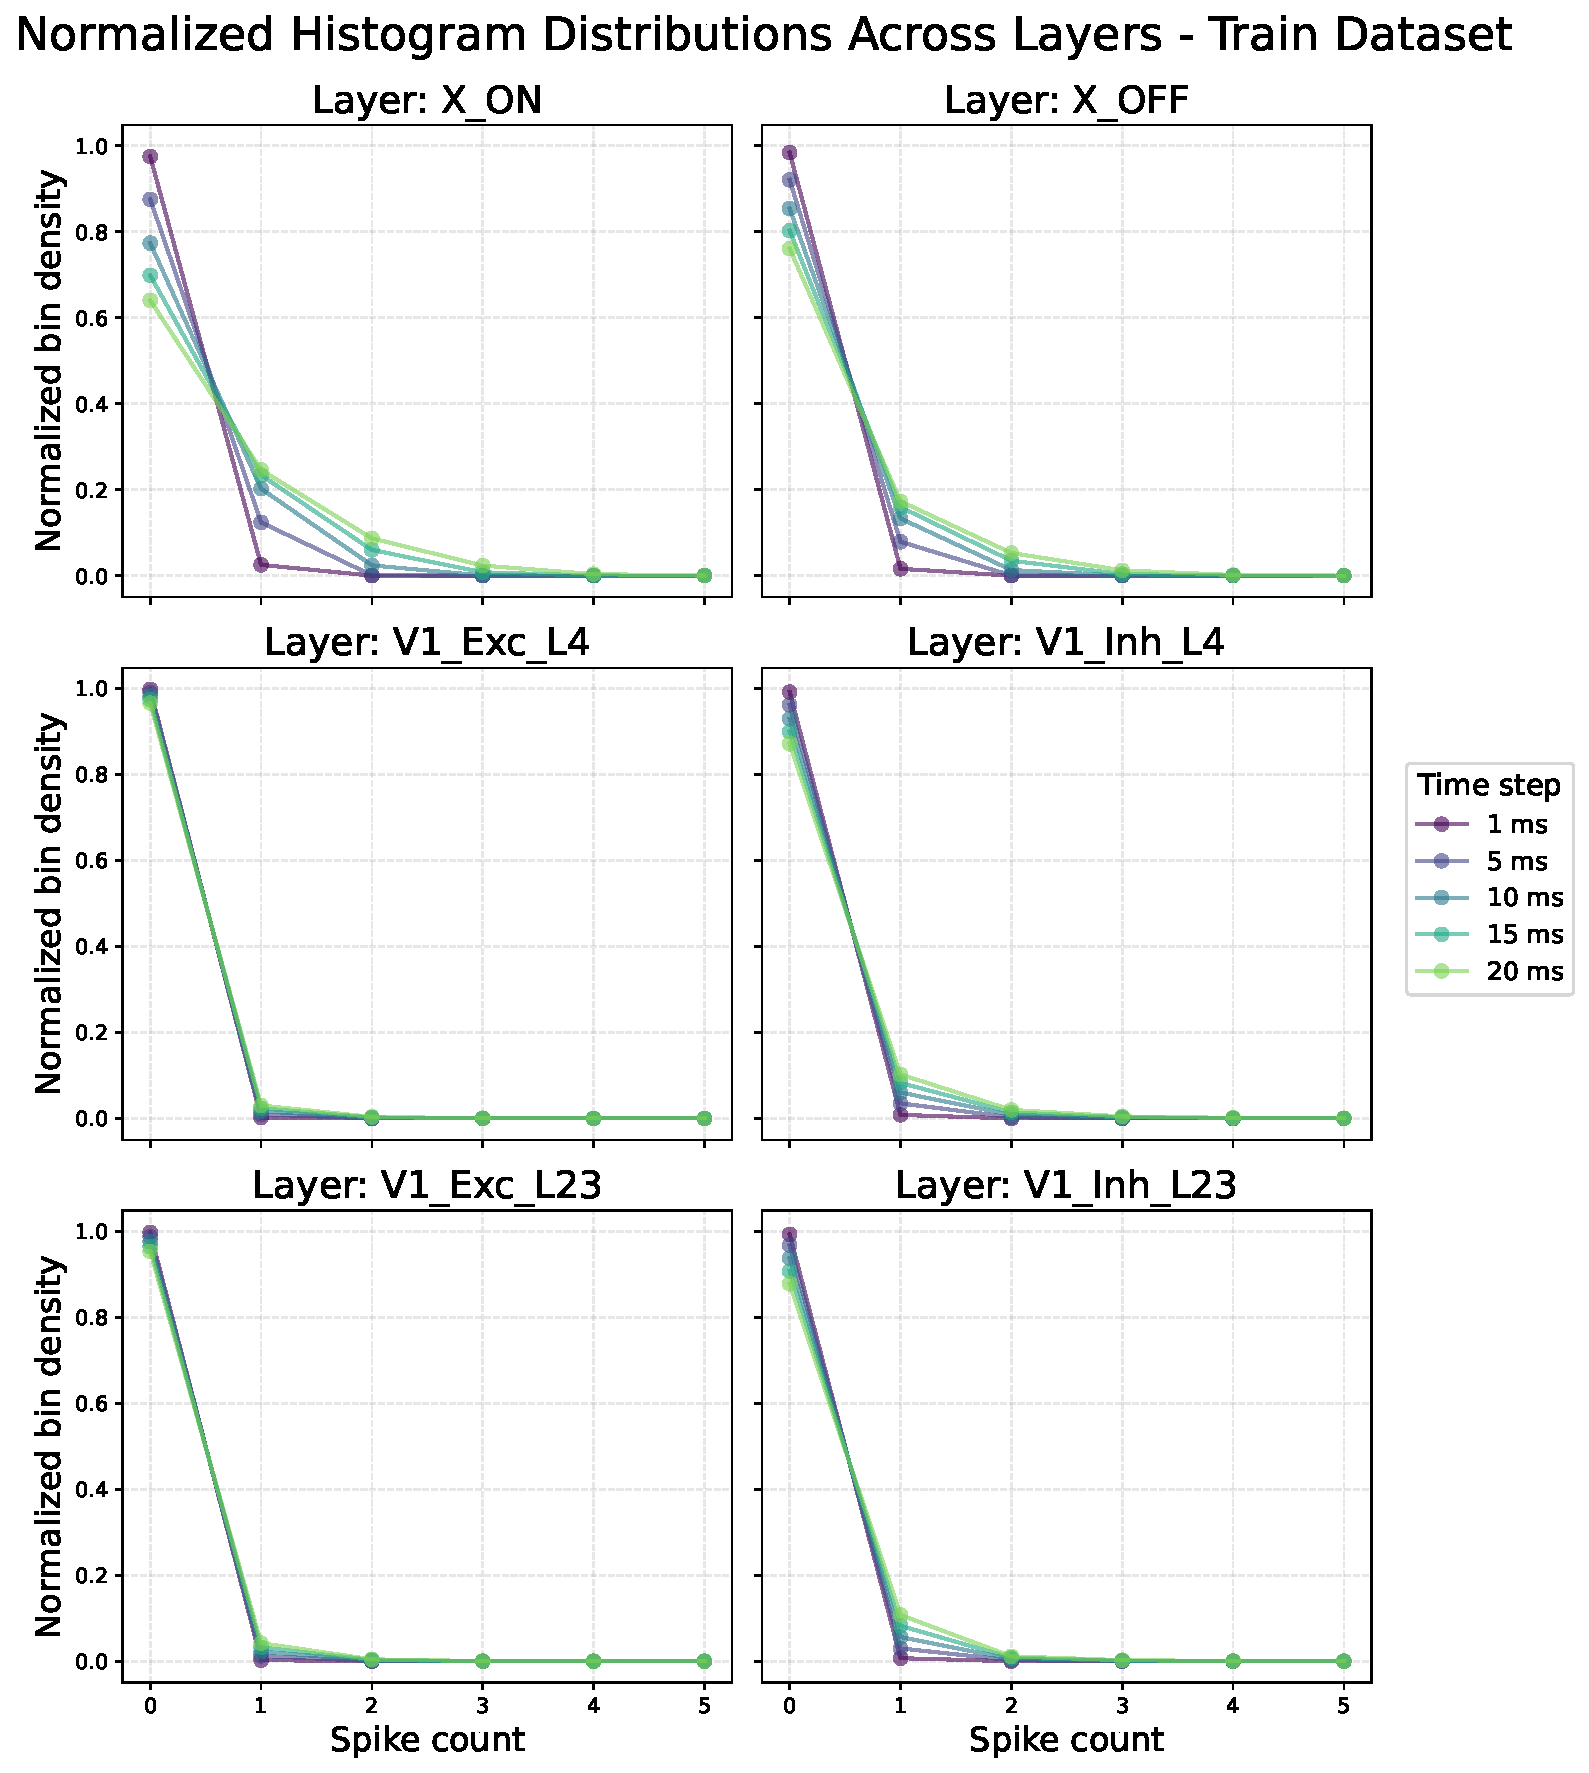
\includegraphics[width=\linewidth]{img/plots/time_step_counts_train.pdf}
    \caption{Evolution of spike counts per time bin with increasing bin size across all neuronal populations in the train dataset.}
    \label{fig:spike_count_distribution_train}
\end{figure}

\begin{figure}
    \centering
    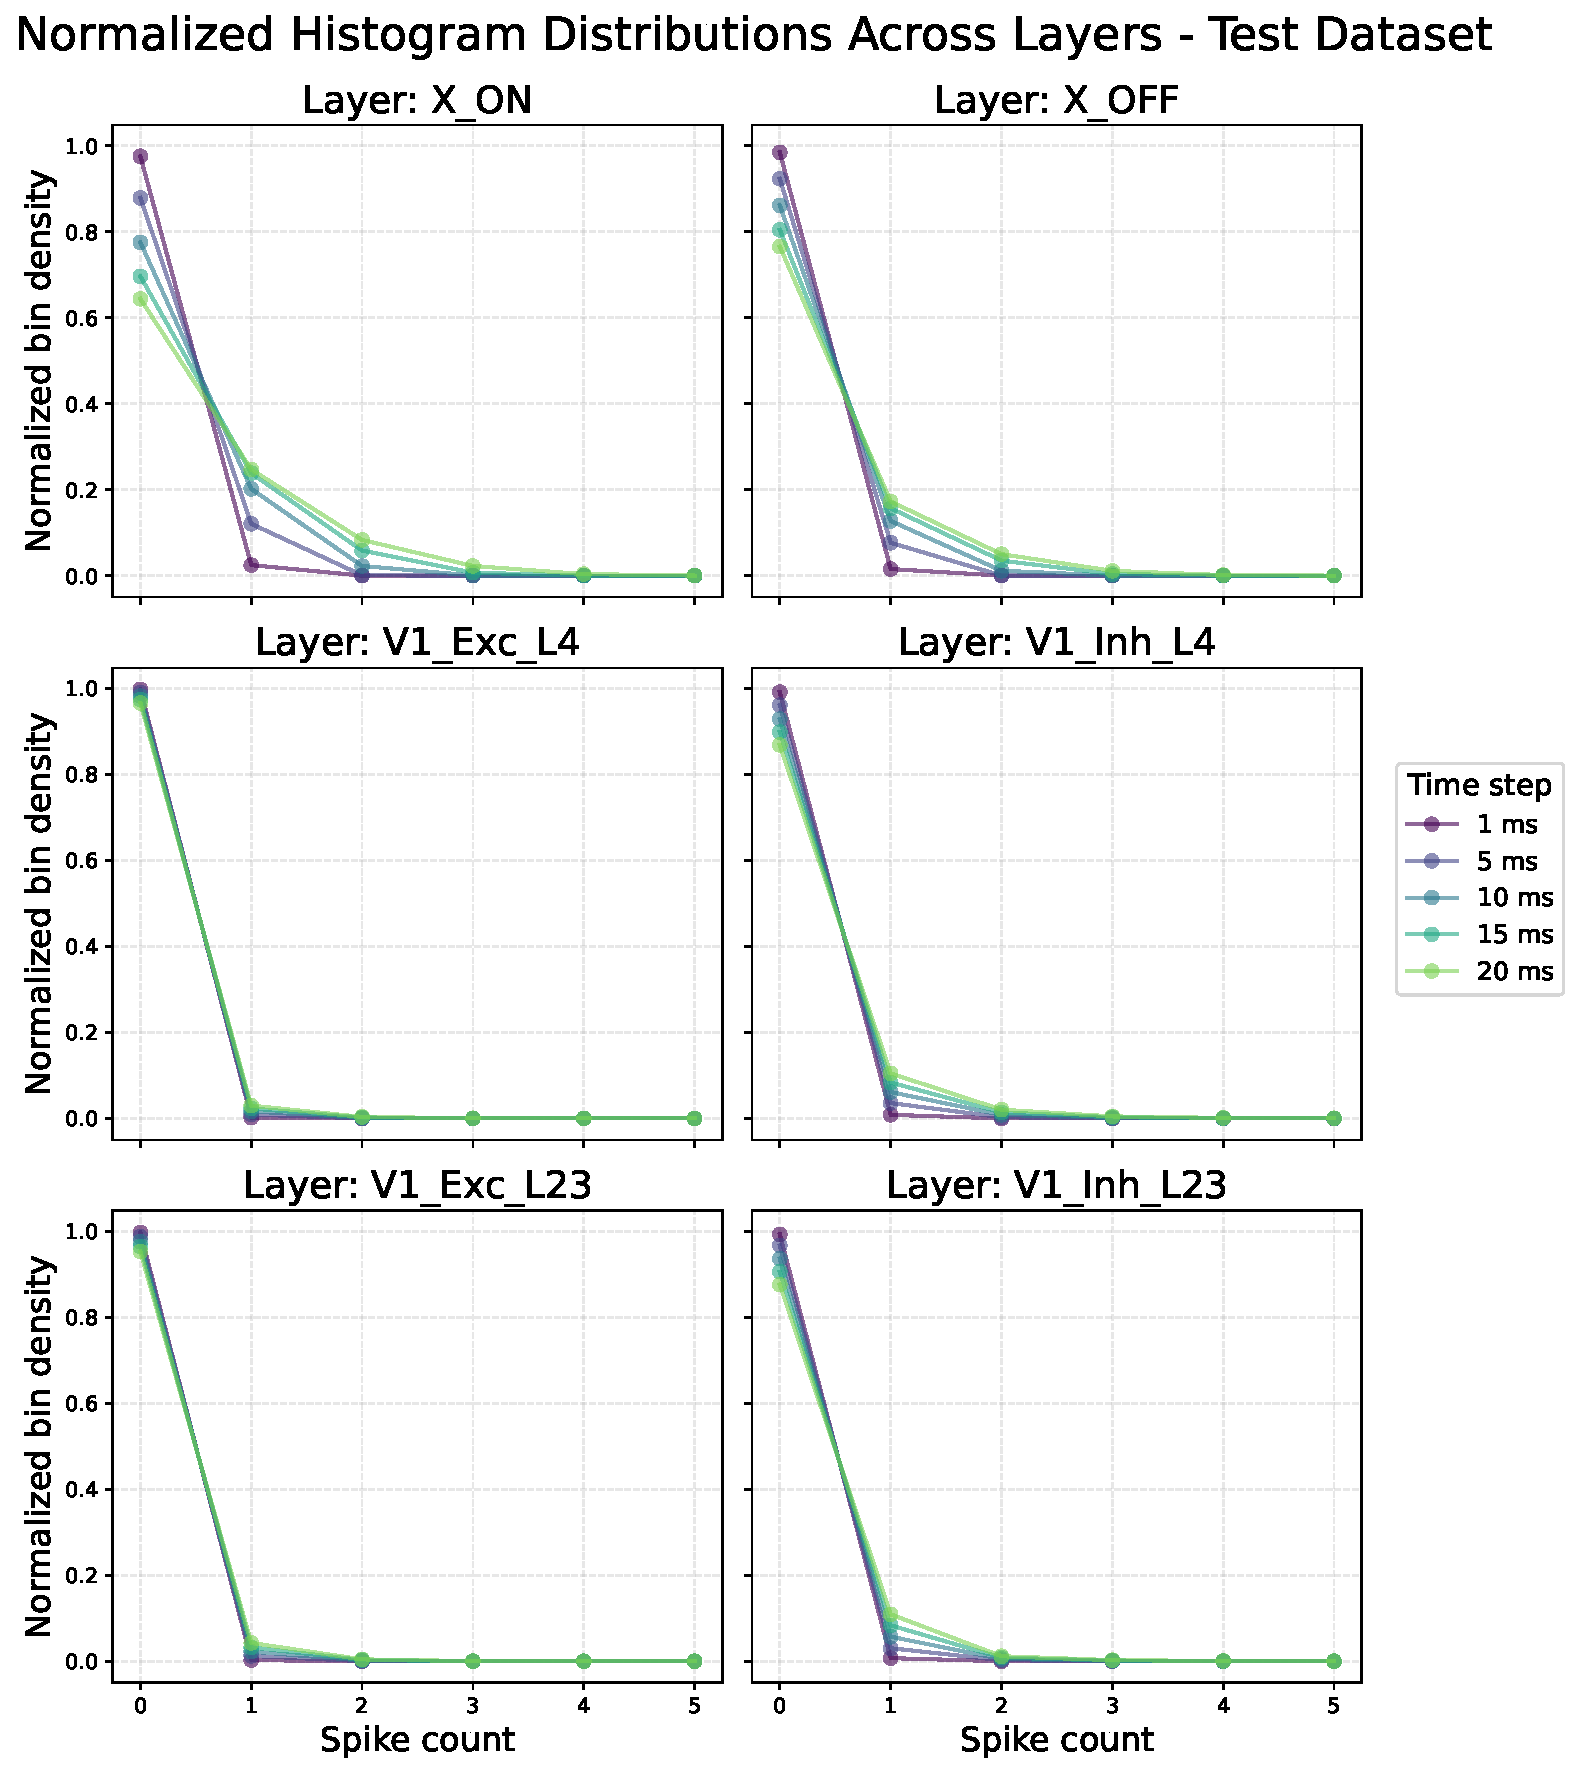
\includegraphics[width=\linewidth]{img/plots/time_step_counts_test.pdf}
    \caption{Evolution of spike counts per time bin with increasing bin size across all neuronal populations in the test dataset.}
    \label{fig:spike_count_distribution_test}
\end{figure}


\subsubsection{Spike Count Distribution Across Time}
\label{subsubsec:spike_time_distribution}
Next, we examine the distribution of spike counts across time for different bin sizes. We propose the following:

\begin{claim}[Temporal Spike Count Distribution]
    The temporal distribution of spike counts per experiment remains consistent across all tested bin sizes. This supports the preservation of temporal response patterns.
\end{claim}

Figures~\ref{fig:temporal_spike_distribution_train} and~\ref{fig:temporal_spike_distribution_test} show the mean spike counts over time for all neuronal populations in the training and test datasets, respectively. These distributions were interpolated to the 1~ms time scale using cubic interpolation.

\begin{figure}
    \centering
    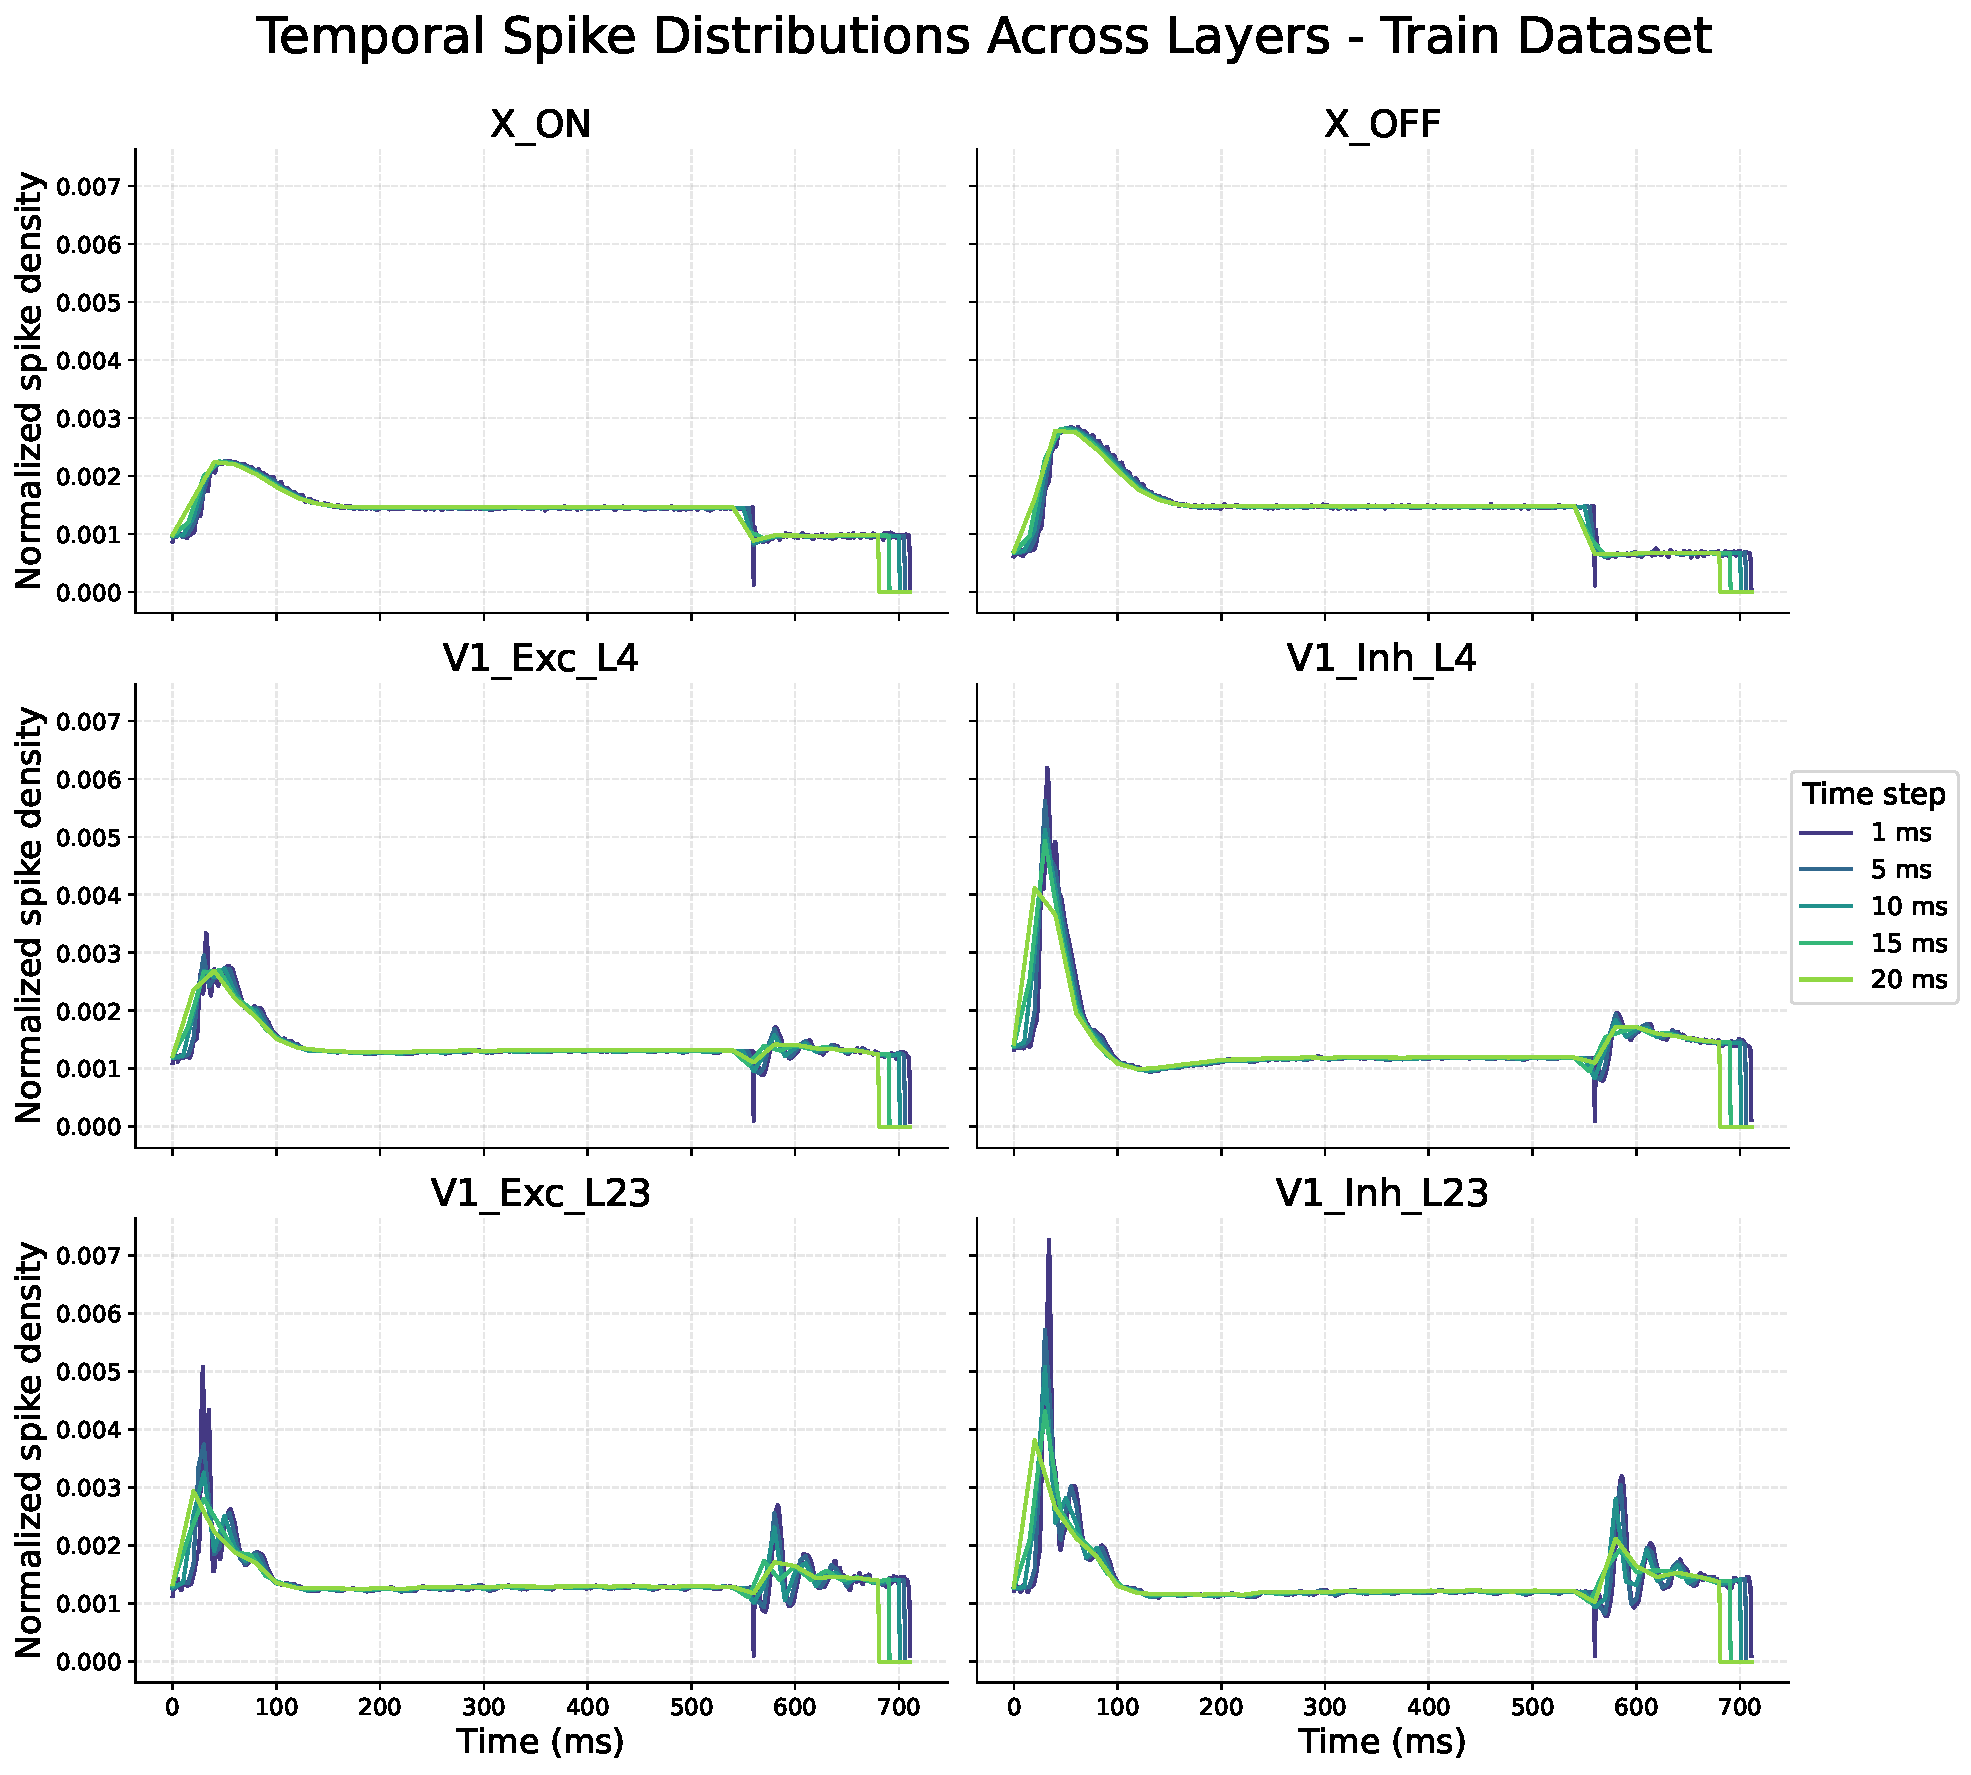
\includegraphics[width=\linewidth]{img/plots/temporal_spike_distribution_train.pdf}
    \caption{Comparison of temporal spike count distributions for different time bin sizes across all neuronal populations in the train dataset. The curves are interpolated to the original 1~ms resolution using cubic interpolation to improve line smoothness.}
    \label{fig:temporal_spike_distribution_train}
\end{figure}

\begin{figure}
    \centering
    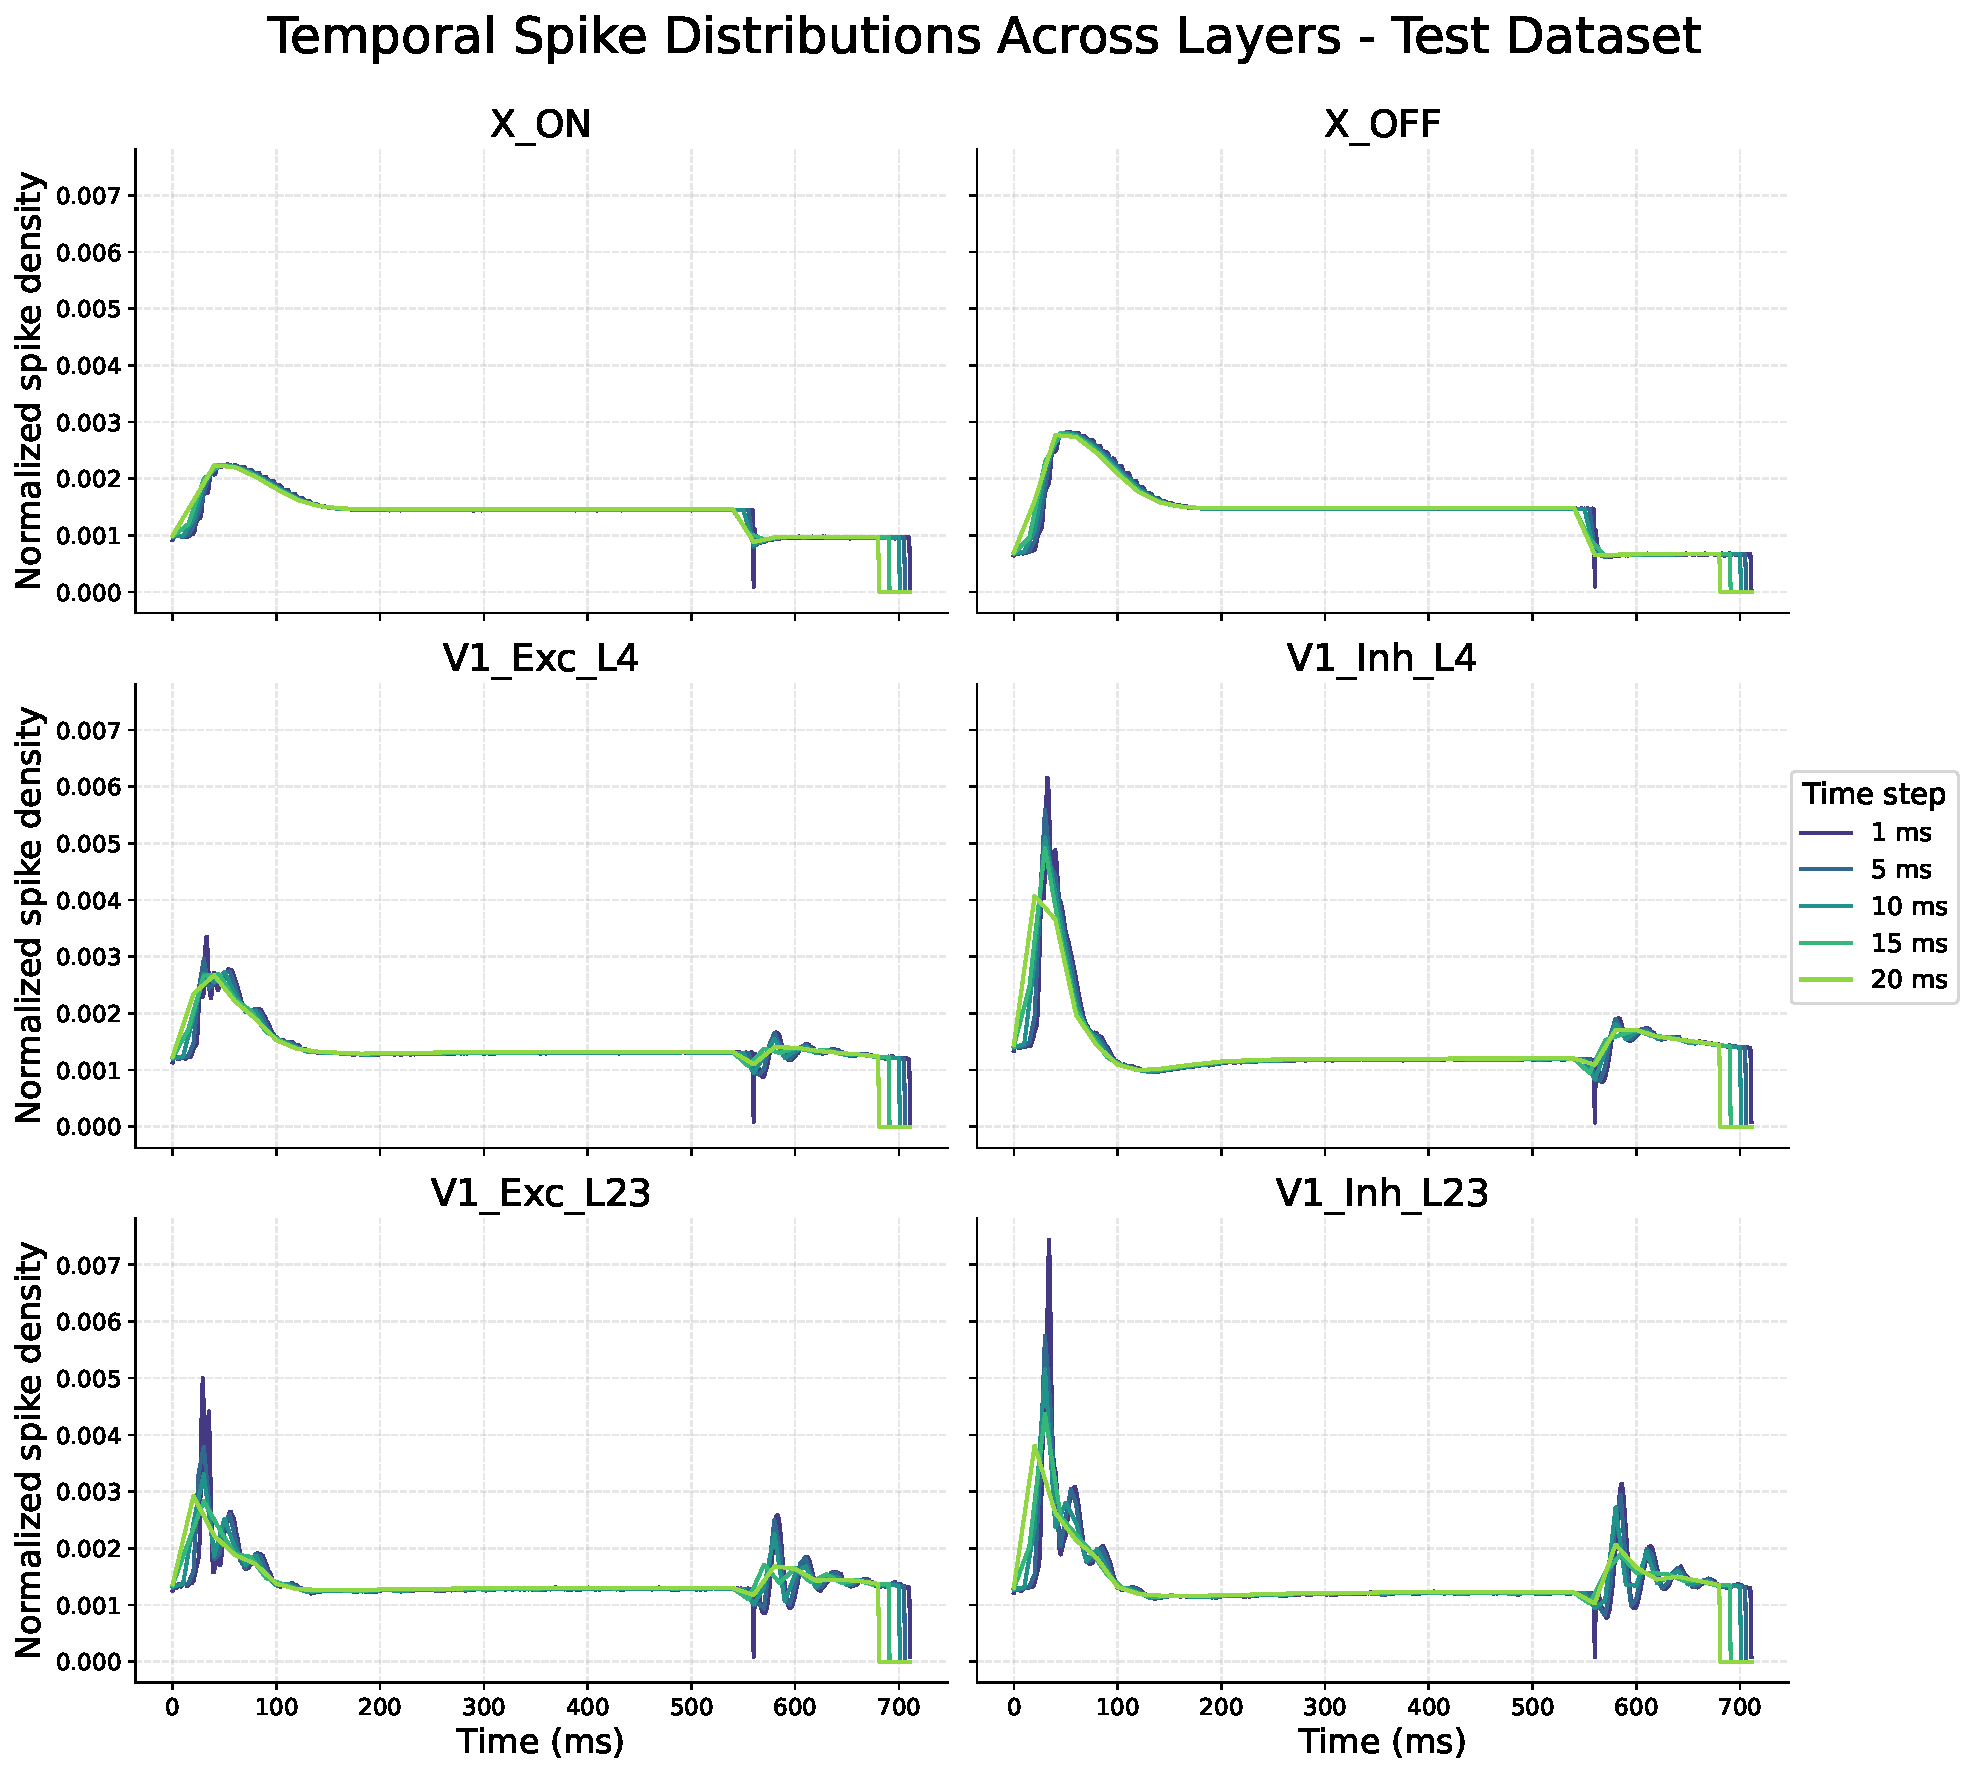
\includegraphics[width=\linewidth]{img/plots/temporal_spike_distribution_test.pdf}
    \caption{Comparison of temporal spike count distributions for different time bin sizes across all neuronal populations in the test dataset. The curves are interpolated to the original 1~ms resolution using cubic interpolation to improve line smoothness.}
    \label{fig:temporal_spike_distribution_test}
\end{figure}

These plots show a clear reduction in noise with increasing bin size, particularly in excitatory layers. The training dataset appears noisier than the test set, likely due to the test set's smaller size and the averaging effect of multiple trials per experiment.

Importantly, the overall distribution shape is preserved across bin sizes. This indicates that binning effectively reduces noise without substantially altering temporal dynamics. Heatmaps in Figure~\ref{fig:correlation_time_bin_size} display Pearson correlation coefficients across different bin sizes, confirming strong similarity in spike distributions over time.

\begin{figure}
    \centering
    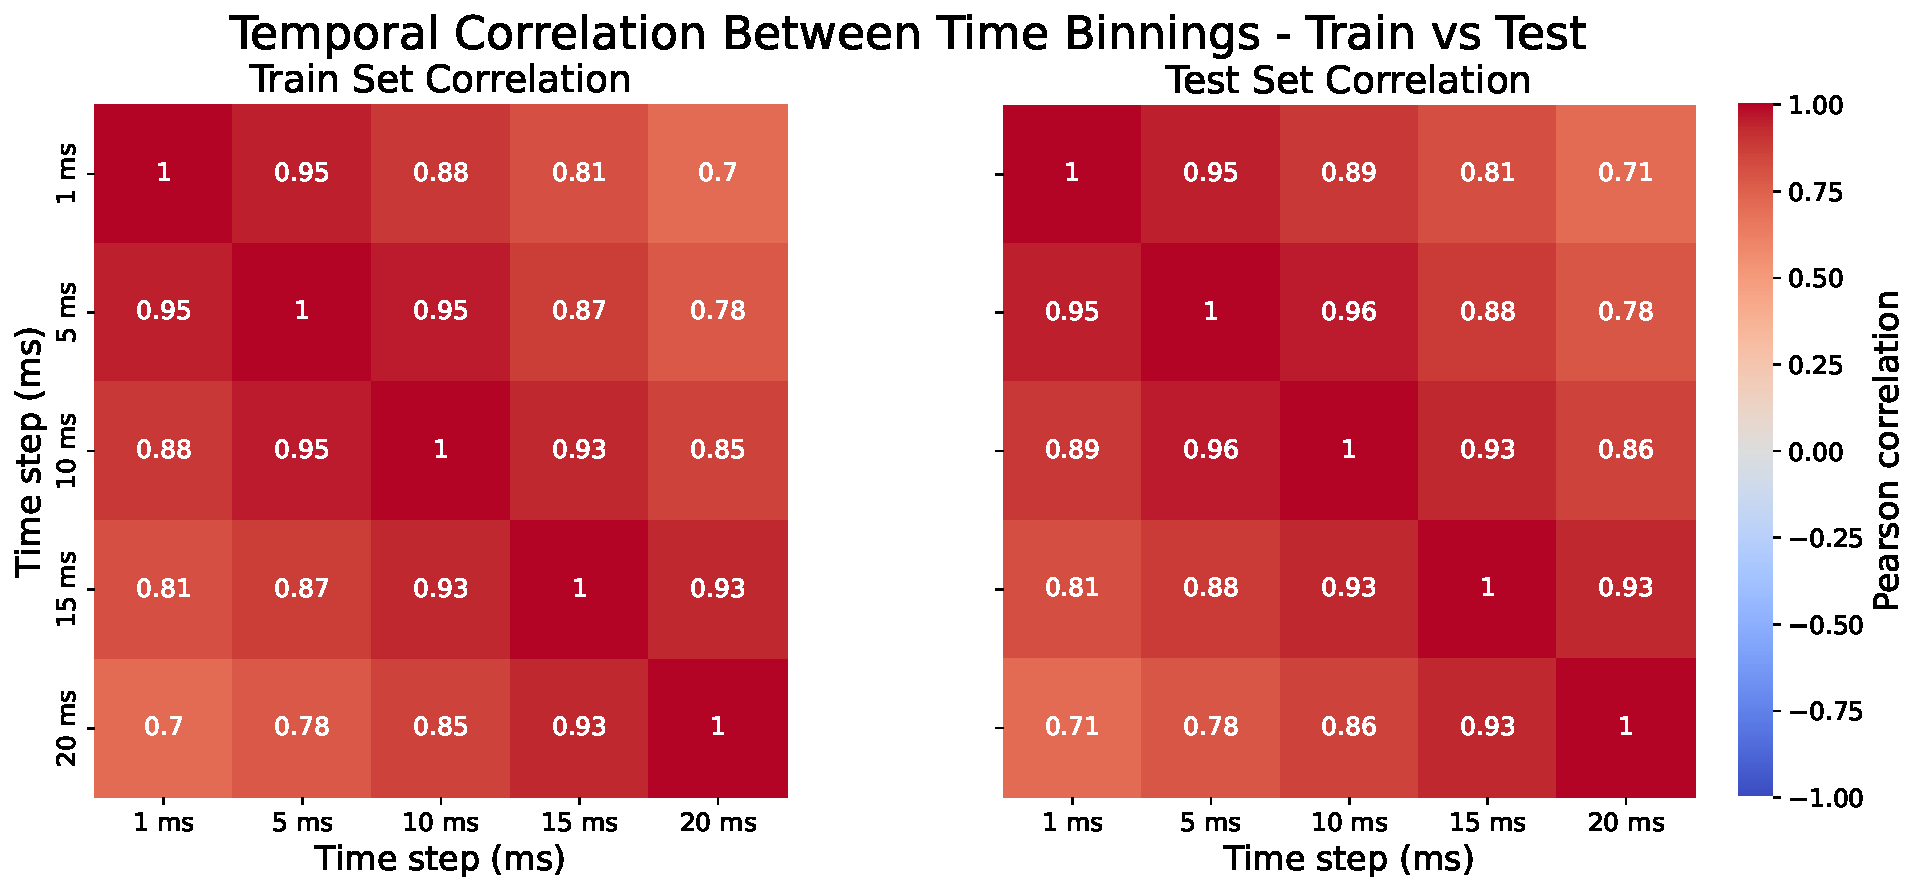
\includegraphics[width=\linewidth]{img/plots/temporal_correlation_time_bin_size.pdf}
    \caption{Heatmaps of Pearson correlation coefficients for spike count distributions over time between different time bin sizes in the train and test datasets.}
    \label{fig:correlation_time_bin_size}
\end{figure}

\subsubsection{Population Spike Count per Time Bin}
\label{subsubsec:neuron_synchrony_binning}

Lastly, we assess how time binning influences the number of neurons spiking simultaneously within a single time bin. Throughout the analysis, we refer to this measure, the proportion of neurons active at each time step, as the \emph{population spike count}. Population spike count provides insight into the collective temporal dynamics of neuronal populations and is widely studied in neuroscience (\citet{Singer1999}).

Our analysis focuses on the mean population spike count across all time steps. We state the following:

\begin{claim}[Population Spike Count of Neuronal Populations Across Time Bins]
    The mean population spike count of neuronal populations remains consistent across different time bin sizes. This implies that temporal structure of the dataset is largely preserved.
\end{claim}
\label{claim:synchrony_time_bins_size}

Figures~\ref{fig:boxplot_synchrony_time_train} and~\ref{fig:boxplot_synchrony_time_test} show population spike count distributions for each layer in the training and test datasets. Tables~\ref{tab:synchrony_time_bins_summary_train} and~\ref{tab:synchrony_time_bins_summary_test} summarize the mean and variance of population spike count values.

\begin{figure}
    \centering
    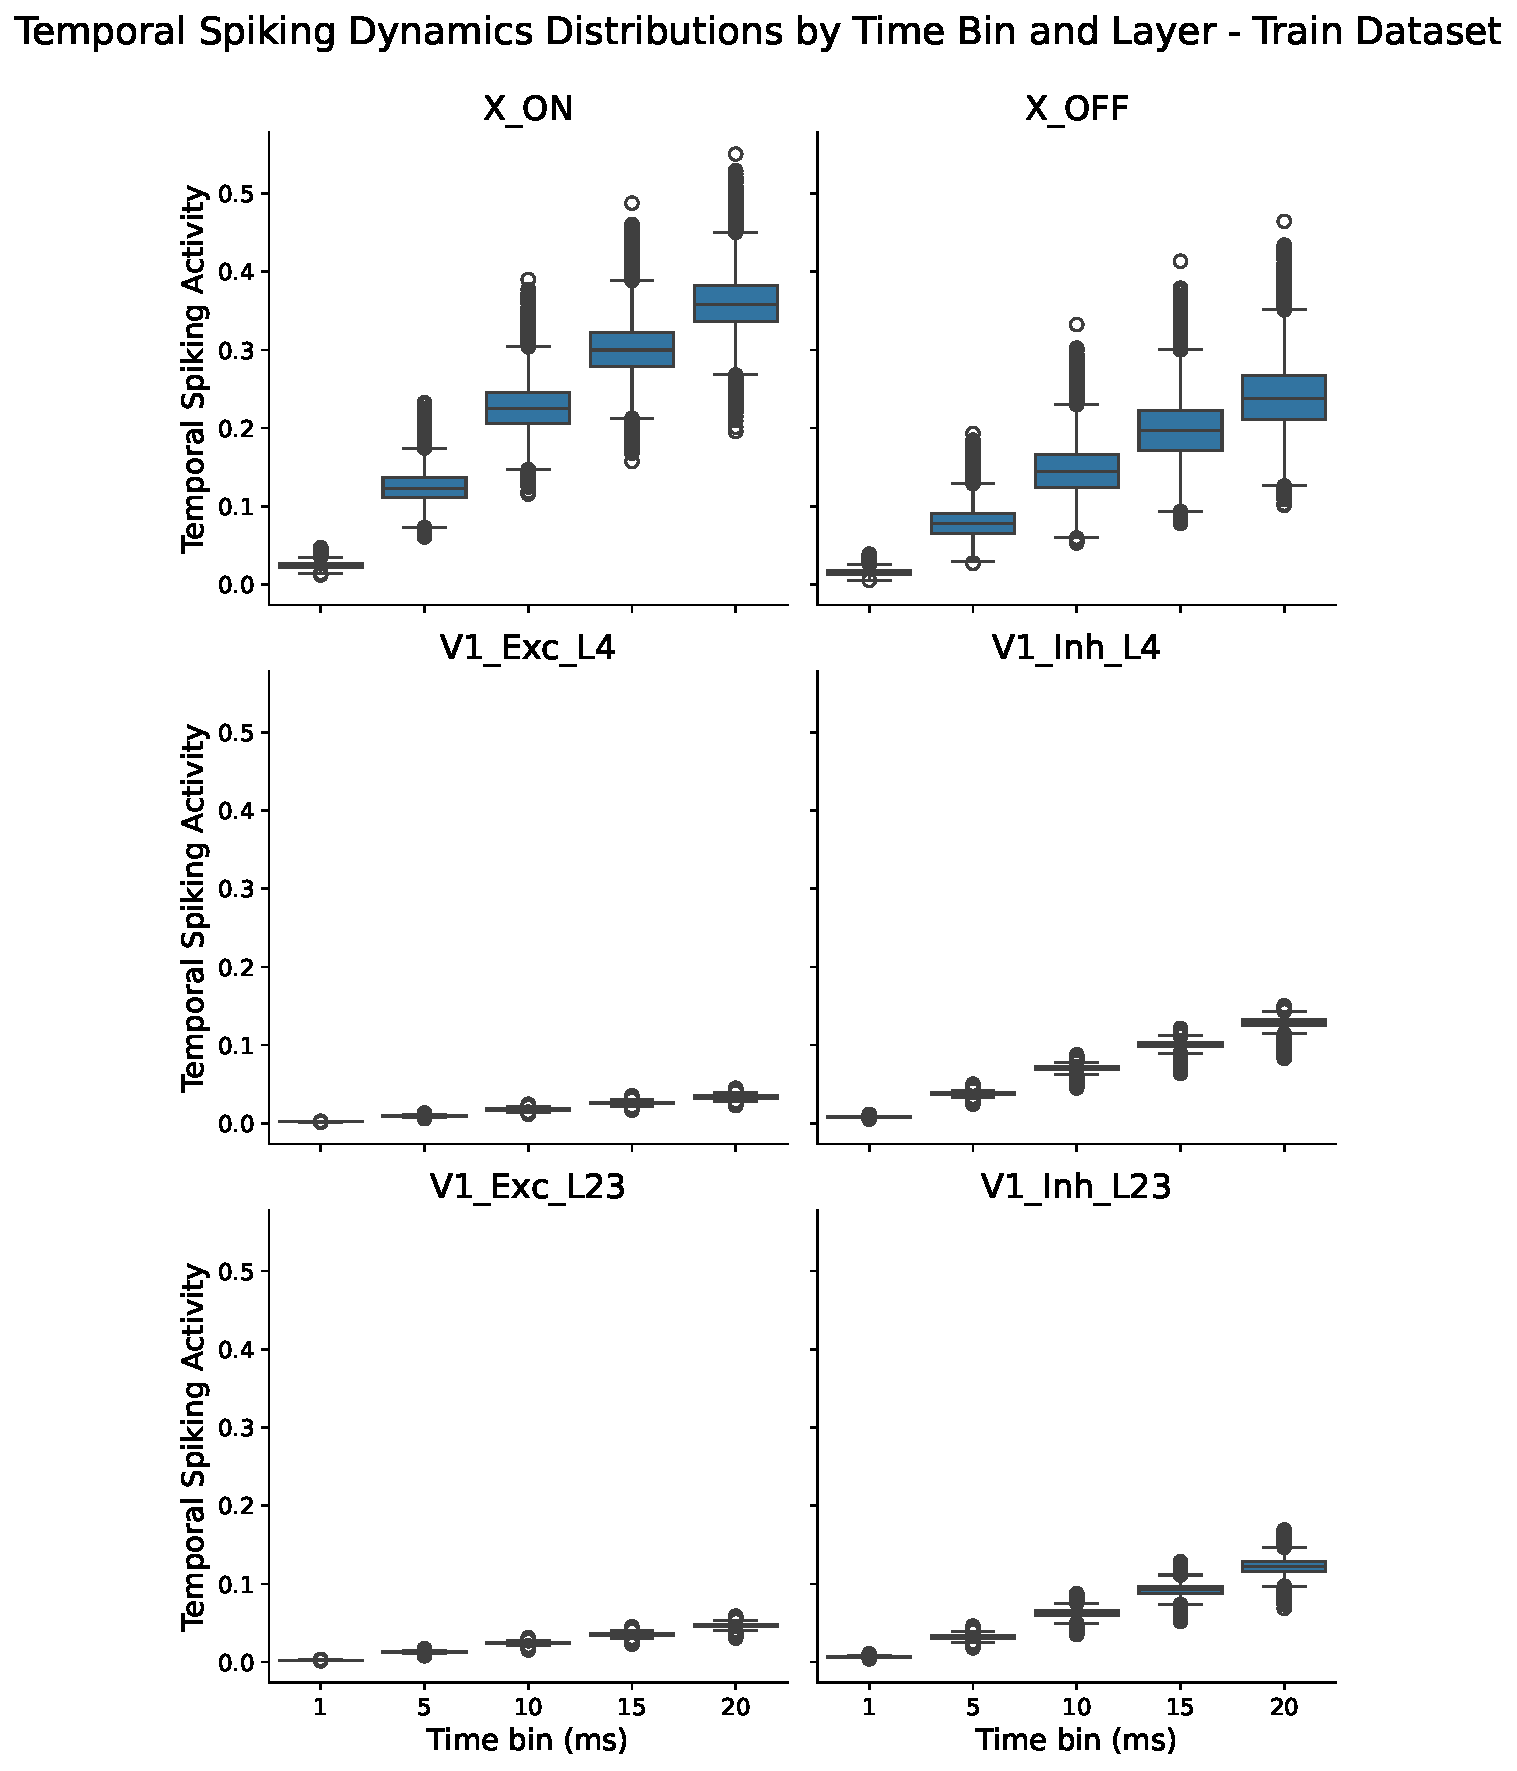
\includegraphics[width=0.92\linewidth]{img/plots/synchrony_boxplot_time_bins_train.pdf}
    \caption{Distribution of mean population spike count across different time bin sizes for all neuronal populations in the train dataset. The boxplot represents the distribution of mean population spike count values calculated across all experiments}
    \label{fig:boxplot_synchrony_time_train}
\end{figure}


\begin{figure}
    \centering
    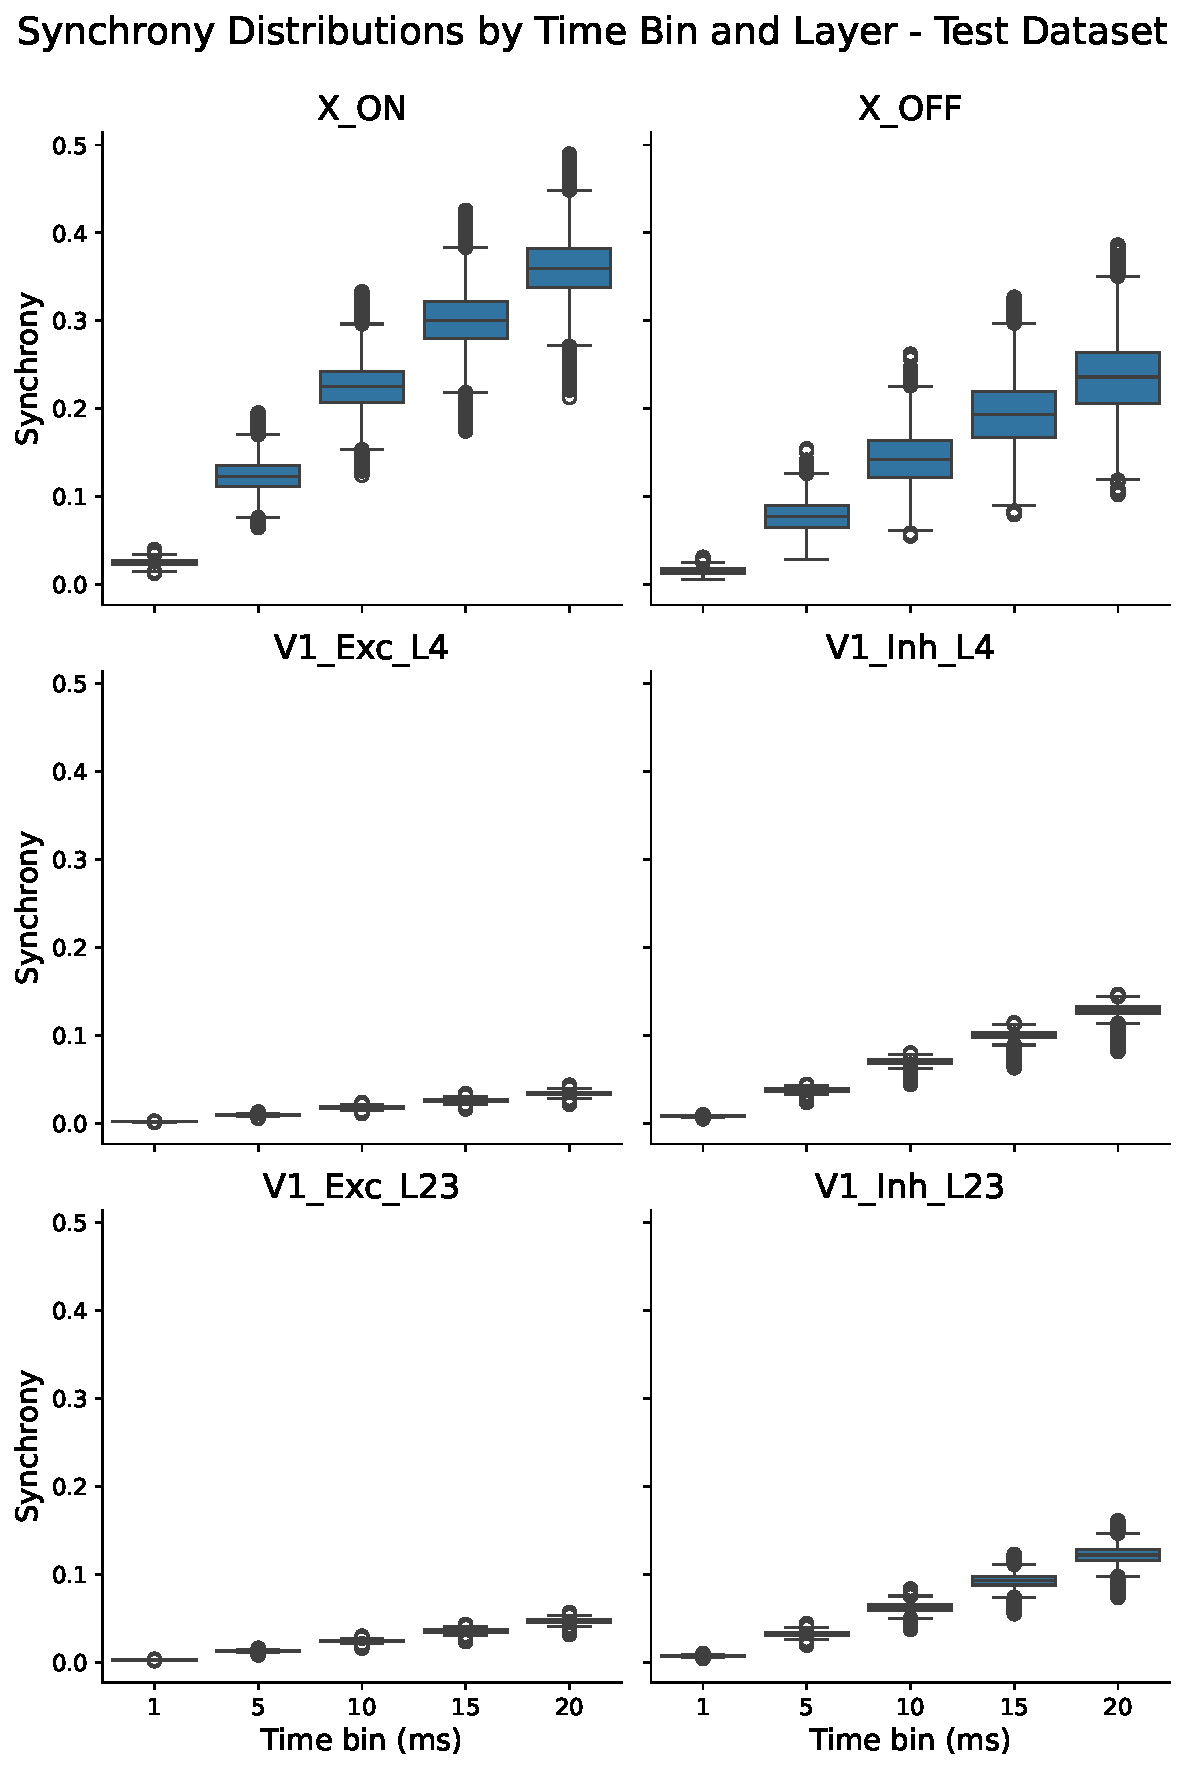
\includegraphics[width=0.92\linewidth]{img/plots/synchrony_boxplot_time_bins_test.pdf}
    \caption{Distribution of mean population spike count across different time bin sizes for all neuronal populations in the test dataset. The boxplot represents the distribution of mean population spike count values calculated across all experiments}
    \label{fig:boxplot_synchrony_time_test}
\end{figure}

\begin{table}
    \centering\footnotesize\sf
    \begin{tabular}{lrr}
    \toprule
    time step & mean & variance \\
    \midrule
    1 & 0.0101 & 0.0001 \\
    5 & 0.0494 & 0.0018 \\
    10 & 0.0912 & 0.0057 \\
    15 & 0.1256 & 0.0098 \\
    20 & 0.1551 & 0.0134 \\
    \addlinespace % a nice non-intrusive separator of data groups (or final table sums)
    \bottomrule
    \end{tabular}
    \caption{\textbf{Summary of population spike count statistics across time bin sizes in the train dataset:} This table reports the mean and variance of population spike count across all layers for each time bin size.}
    \label{tab:synchrony_time_bins_summary_train}
\end{table}

\begin{table}
    \centering\footnotesize\sf
    \begin{tabular}{lrr}
    \toprule
    time step & mean & variance \\
    \midrule
    1 & 0.0101 & 0.0001 \\
    5 & 0.0491 & 0.0017 \\
    10 & 0.0908 & 0.0057 \\
    15 & 0.1250 & 0.0097 \\
    20 & 0.1545 & 0.0133 \\
    \addlinespace % a nice non-intrusive separator of data groups (or final table sums)
    \bottomrule
    \end{tabular}
    \caption{\textbf{Summary of population spike count statistics across time bin sizes in the test dataset:} This table reports the mean and variance of population spike count across all layers for each time bin size.}
    \label{tab:synchrony_time_bins_summary_test}
\end{table}

Population spike count increases with larger time bins, reflecting a higher likelihood of coincident spiking. This effect is most pronounced in LGN layers, especially X\_ON, while V1 excitatory layers show a milder change.

Based on these findings, we conclude that a binning size of 20~ms influences the temporal dynamics of neuronal responses and may consequently affect the resulting neuronal predictions. However, due to the computational complexity of our task, it was not feasible to develop and train models using a smaller time bin size. Therefore, this limitation must be carefully considered during both model development and the interpretation of results.

\subsection{Model Subset Selection Analysis}
\label{subsec:subset_selection_analysis}

In this section, we analyze the impact of selecting a subset of neurons from the original SNN model. As discussed in Section~\ref{subsubsec:subset_selection}, we selected only 10\% of the neurons due to memory constraints and the computational demands of model training. Our primary interest lies in assessing how this subset selection affects the temporal properties of the dataset, which are central to our research.

All experiments in this section are conducted on the dataset with a 20~ms time bin size (as used in our model) and focus on the training dataset unless stated otherwise. As shown previously in Section~\ref{subsubsec:time_bins_merging}, the results from the training and test datasets are largely consistent.

\subsubsection{Total Spike Counts Across Time Bins}
\label{subsubsec:total_spike_counts_subset}
We begin by analyzing the distribution of spike counts in the time bins for the full dataset and for the subset datasets. Table~\ref{tab:subset_spike_count_distribution} summarizes the mean spike count ratios across all model subsets compared to the full dataset.

\begin{table}
    \centering\footnotesize\sf
    \begin{tabular}{rrrr}
        \toprule
        Spike Count & Full Dataset Ratio & Subsets Mean Ratio & Subsets Standard Deviation \\
        \midrule
        0 & 0.9105 & 0.9102 & 0.0004 \\
        1 & 0.0710 & 0.0712 & 0.0003 \\
        2 & 0.0147 & 0.0148 & 0.0001 \\
        3 & 0.0032 & 0.0032 & 0.0000 \\
        4 & 0.0005 & 0.0005 & 0.0000 \\
        5 & 0.0001 & 0.0001 & 0.0000 \\
        \bottomrule
    \end{tabular}
    \caption{\textbf{Comparison of spike count distributions between full and subset datasets:} This table presents the mean spike count ratios and standard deviations across all model subsets, relative to the full dataset.}
    \label{tab:subset_spike_count_distribution}
\end{table}

The table shows that the differences in spike count distributions between the full and subset datasets are minimal, with low standard deviations. This suggests that randomly selecting a subset of neurons does not significantly impact the overall spike count distribution.

\subsubsection{Spike Count Distribution Across Time}
\label{subsubsec:spike_time_distribution_subset}

Next, we compare the temporal spike count distributions of the subset datasets with that of the full dataset. Figure~\ref{fig:temporal_distribution_subset_vs_full_train} shows the mean temporal behavior across layers for both the full dataset and the average of all subsets. The shaded area represents the standard deviation across subsets.
\begin{figure}
    \centering
    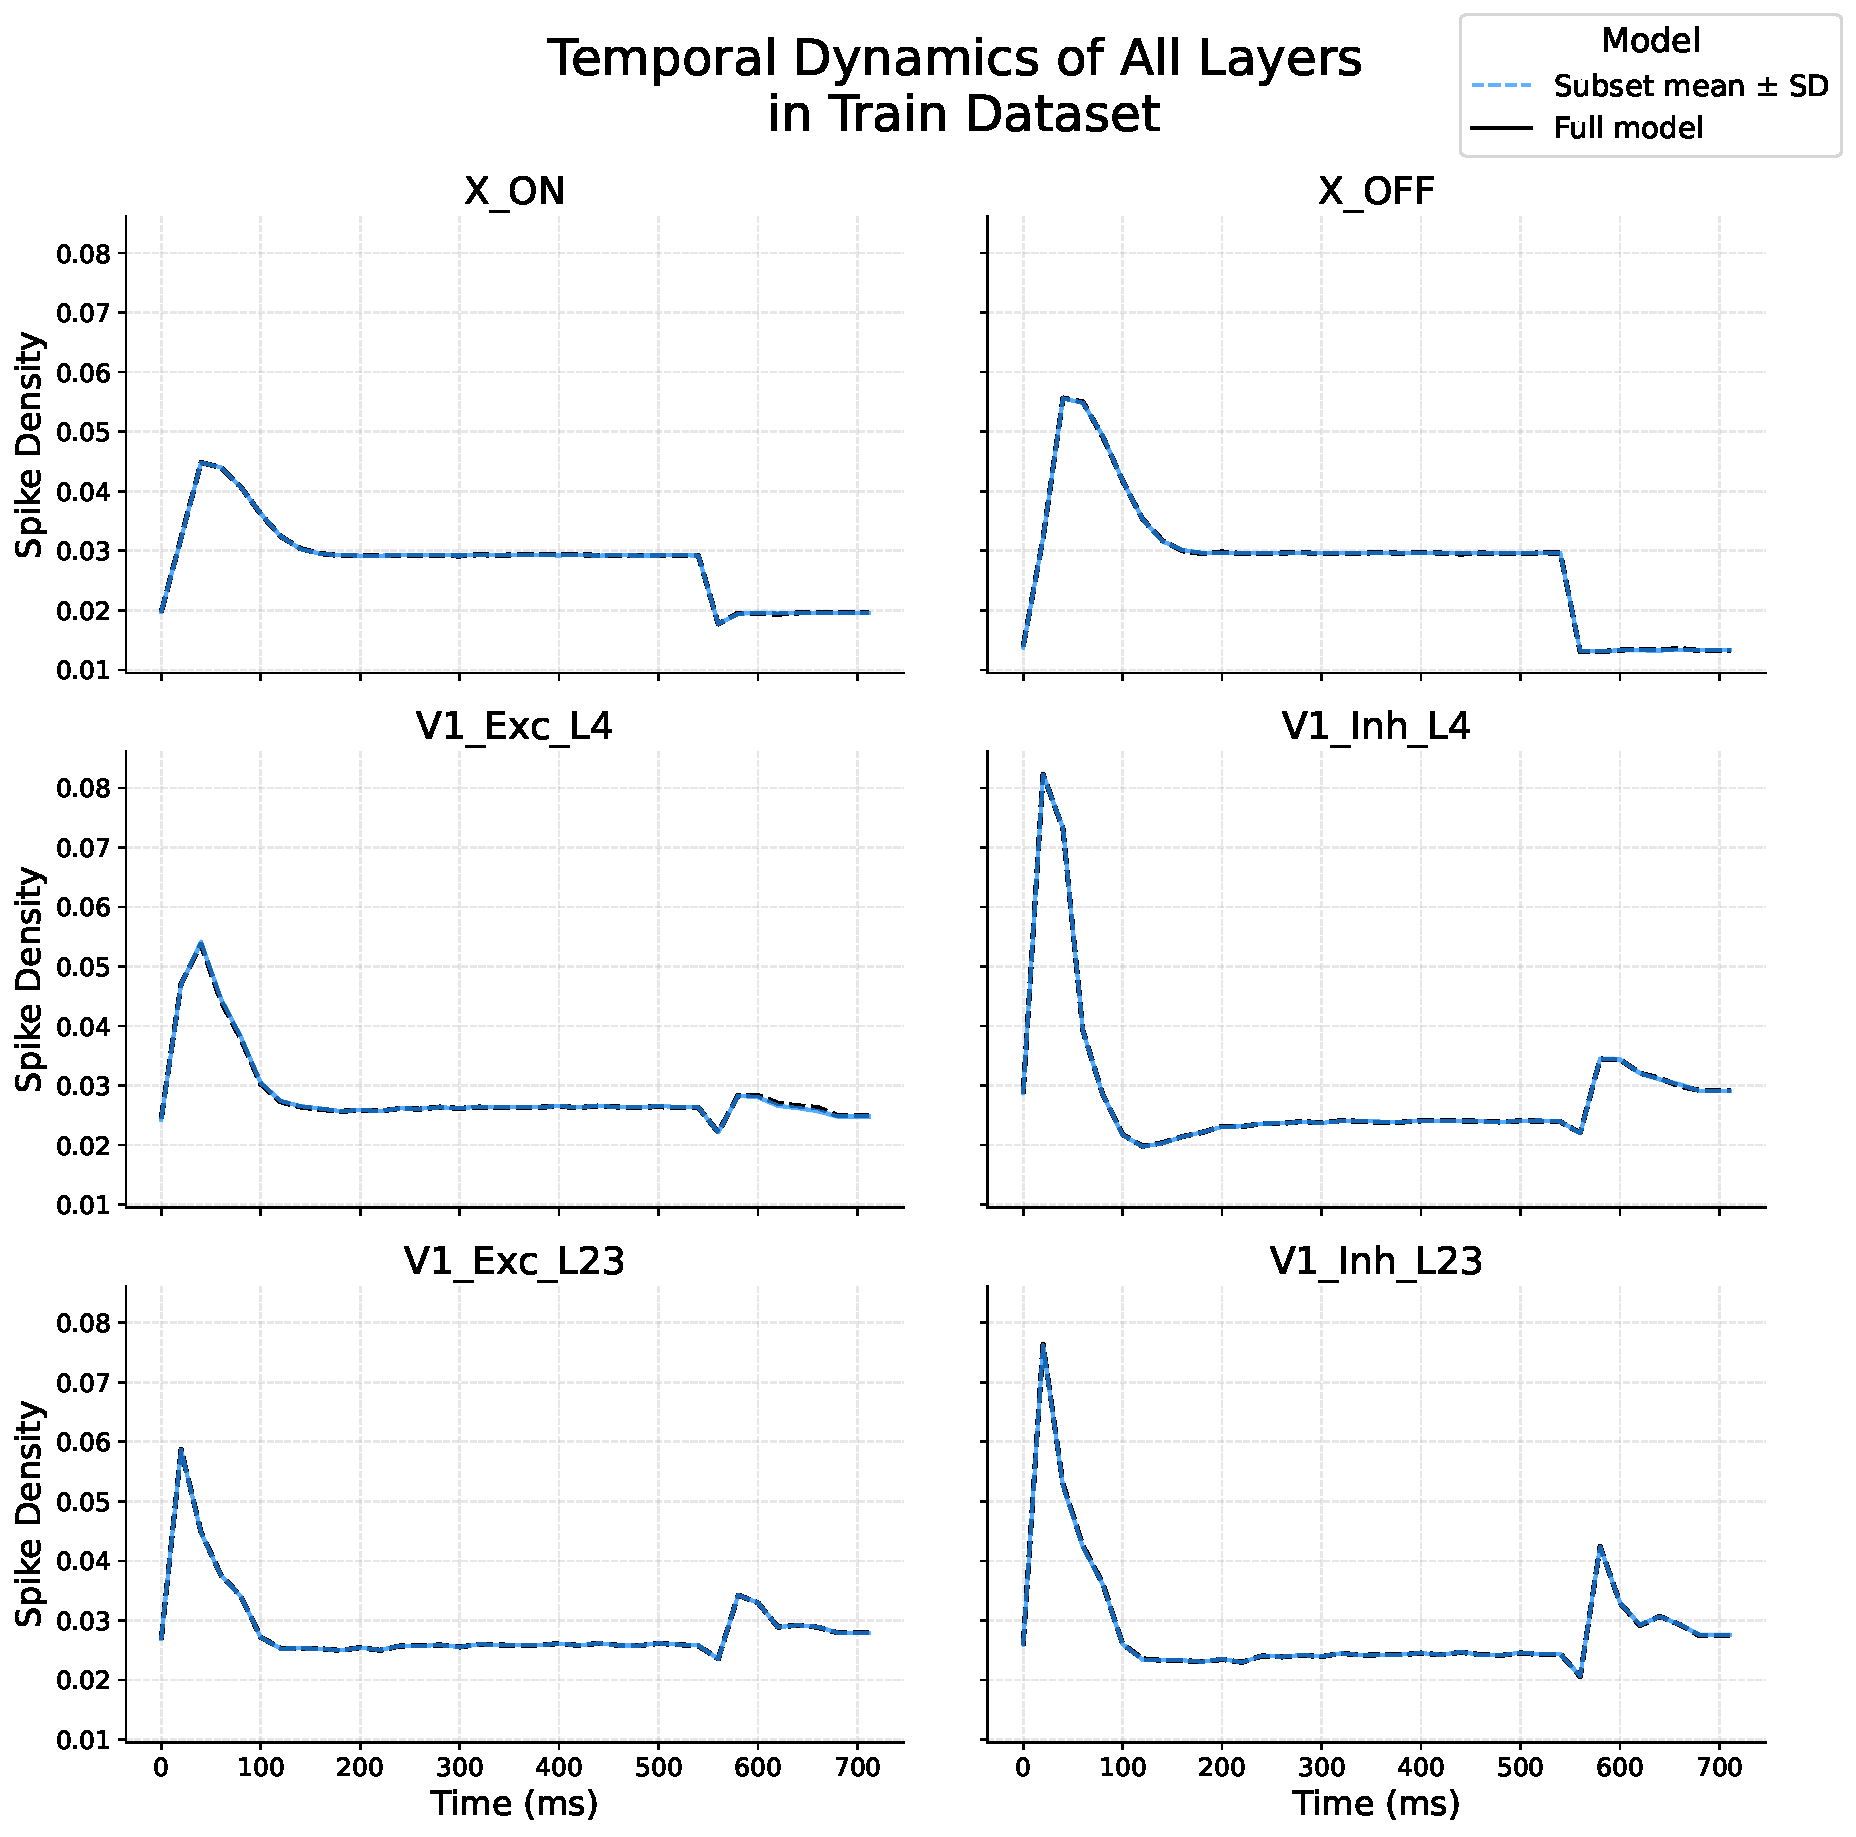
\includegraphics[width=\linewidth]{img/plots/temporal_distribution_subset_vs_full_train.pdf}
    \caption{Comparison of mean temporal activity across layers for the full dataset and the average of all subsets. The shaded area indicates the standard deviation across subsets, which is very small and therefore barely visible in the plot.}
    \label{fig:temporal_distribution_subset_vs_full_train}
\end{figure}

The plot demonstrates that the mean temporal patterns of the subsets closely match those of the full dataset. The small standard deviation further confirms that the temporal properties are preserved despite the neuron subset selection.


\subsubsection{Population spike count of Neuronal Populations in Subsets}
\label{subsubsec:neuron_synchrony_subset}
Finally, we assess the effect of subset selection on neuronal population spike count. Since we are using only a portion of the neurons from the full model, it is possible that groups of neurons that typically spike together may be disrupted, potentially affecting population spike count.

Figure~\ref{fig:boxplot_synchrony_subset} displays a boxplot and jitter plot comparing the population spike count values of the full dataset and all subsets.

\begin{figure}
    \centering
    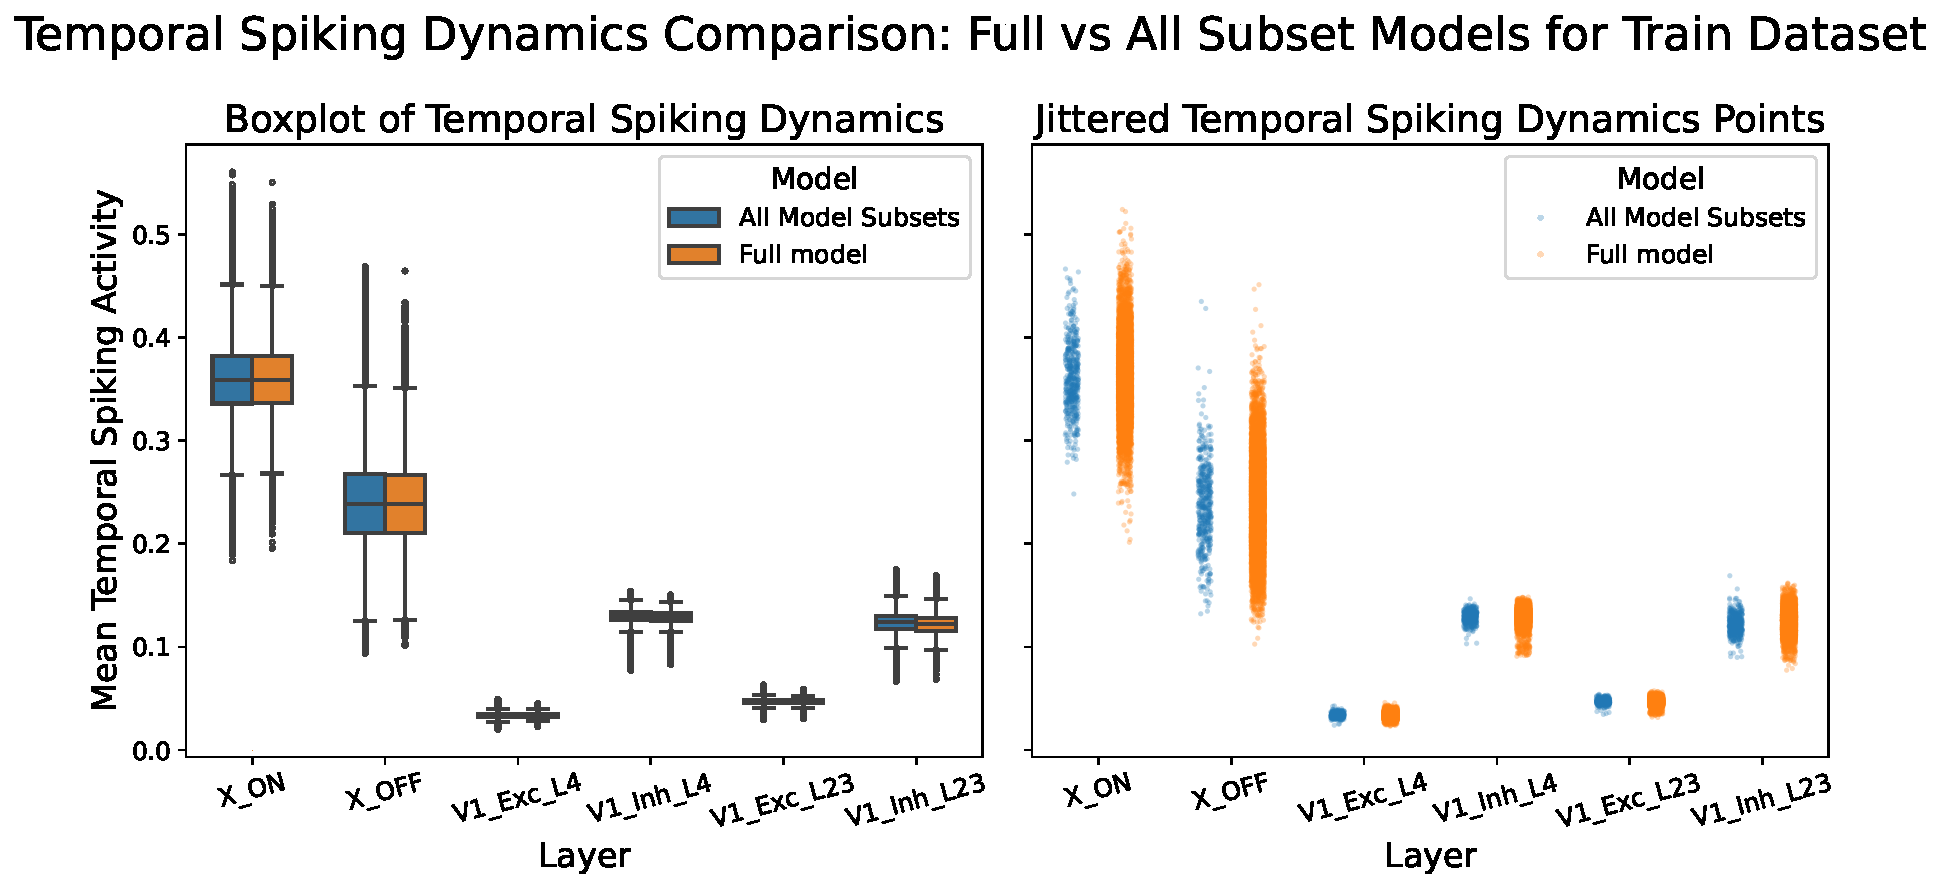
\includegraphics[width=\linewidth]{img/plots/synchrony_comparison_subset_full_train.pdf}
    \caption{Boxplot and jitter plot comparing population population spike count values between the full dataset and all subsets. Each data point represents the mean population spike count of one experiment.}
    \label{fig:boxplot_synchrony_subset}
\end{figure}

As shown, the population spike count distributions are largely similar, particularly in the excitatory layers. This aligns with earlier findings that population spike count variance was low across time bins. Although the jitter plot suggests a slightly narrower spread in the LGN layers for the subsets, the boxplots do not indicate a significant difference.

Based on these observations, we conclude that random selection of 10\% of neurons from the full SNN model does not substantially affect the dataset's statistical or temporal properties. Nevertheless, slight changes in population spike count, particularly in LGN layers, should be taken into account when interpreting model performance results.

\section{Model Evaluation}
\label{sec:model_evaluation}

This section evaluates the performance of our models by comparing different versions and analyzing how each additional module influences the results. We start with a high-level comparison of all model variants, then examine individual performances, and finally discuss the limitations and possible causes of prediction errors.

Unless noted otherwise, all results are aggregated across 20 randomly selected neuronal sub-populations, each representing 10\% of the original dataset. This selection method, described in Section~\ref{subsubsec:subset_selection}, helps reduce bias and better reflect overall model behavior.

We follow a consistent naming convention for the models, primarily based on definitions in Section~\ref{sec:model_description}. However, to distinguish between certain configurations, we introduce some new labels:

\begin{itemize}
    \item \textbf{simple (tanh)}: A simple model with a tanh activation function (Section~\ref{subsec:base_model_architecture}).
    \item \textbf{simple (leakytanh)}: A simple model using a leakytanh activation function (Section~\ref{subsubsec:leakytanh}).
    \item \textbf{dnn joint}: A model using feed-forward joint neuron modules (Section~\ref{subsubsec:dnn_neuron}).
    \item \textbf{dnn separate}: A model using feed-forward separate neuron modules  (Section~\ref{subsubsec:dnn_separate}).
    \item \textbf{rnn (5 steps)}: A model using RNN neuron modules with 5 TBPTT (Truncated Backpropagation Through Time) steps (Section~\ref{subsubsec:rnn_neuron_module}).
    \item \textbf{rnn (10 steps)}: A model using RNN neuron modules with 10 TBPTT steps.
    \item \textbf{syn adapt lgn (5 steps)}: A model using RNN neuron modules also with synaptic depression modules applied only to LGN connections, using 5 TBPTT steps (Section~\ref{subsubsec:synaptic_depression}). The term \textit{adapt} refers to the naming in our implementation of the module.
\end{itemize}

All models were trained and evaluated using the general setup outlined in Section~\ref{sec:experimental_setup}. Specific hyperparameters for each model are listed in Table~\ref{tab:evaluation_setup}. These parameters were primarily selected through grid search, supplemented by empirical tuning based on development experience. More details on this process will follow in subsequent sections.

\begin{table}
    \centering\footnotesize\sf
    \begin{tabular}{lrrrrrrrr}
        \toprule
        Model Variant & Epochs & lr & n-ls & n-nl & n-res & s-ls & s-nl & n-tbptt \\
        \midrule
        simple (tanh) & 10 & 0.000008 & - & - & - & - & - & - \\
        simple (leakytanh) & 10 & 0.000075 & - & - & - & - & - & - \\
        dnn joint & 10 & 0.000010 & 10 & 5 & True & - & - & - \\
        dnn separate & 10 & 0.000010 & 10 & 5 & True & - & - & - \\
        rnn (steps 5) & 40 & 0.000030 & 10 & 3 & True & - & - & 5 \\
        rnn (steps 10) & 40 & 0.000030 & 10 & 3 & True & - & - & 10 \\
        syn adapt lgn (steps 5) & 40 & 0.000030 & 10 & 3 & True & 10 & 2 & 5 \\
        \bottomrule
        \end{tabular}
    \caption{\textbf{Model Setup for Evaluation:} Configuration of each model variant used during evaluation. "Model Variant" indicates the model type. Other columns: "Epochs" - number of training epochs, "lr" - learning rate, "n-ls" - neuron module layer size, "n-nl" - number of layers in the neuron module, "n-res" - whether residual connections are used in the neuron module, "s-ls" - synaptic depression module layer size, "s-nl" - number of layers in the synaptic depression module, "n-tbptt" - number of TBPTT steps. A dash ("-") means the value is not applicable for that model.}
    \label{tab:evaluation_setup}
\end{table}

\subsection{Comparative Evaluation of Model Types}
\label{subsec:overall_model_types_comparison}
This section provides a comparative analysis of all model variants using global performance metrics.

We begin by evaluating each model's performance using Pearson correlation coefficients and normalized cross-correlations, as detailed in Sections~\ref{subsec:pearson_cc} and~\ref{subsec:normalized_cross_correlation}. Table~\ref{tab:model_evaluation_overview_comparison} presents the summary statistics for each model, while Figure~\ref{fig:model_types_correlation_comparison} visualizes the distribution of Pearson and normalized cross-correlation values across all model subset variants.

\begin{table}
    \centering\footnotesize\sf
    \begin{tabular}{lrrrrrrrr}
        \toprule
        Model Variant & N-CC (mean) & P-CC (mean) & N-CC (std) & P-CC (std) \\
        \midrule
        rnn (10 steps) & 0.9212 & 0.7500 & 0.0084 & 0.0082 \\
        rnn (5 steps) & 0.9176 & 0.7471 & 0.0103 & 0.0089 \\
        syn adapt lgn (5 steps) & 0.8935 & 0.7275 & 0.0043 & 0.0042 \\
        dnn joint & 0.8803 & 0.7168 & 0.0021 & 0.0034 \\
        simple (leakytanh) & 0.8778 & 0.7147 & 0.0014 & 0.0032 \\
        dnn separate & 0.8430 & 0.6864 & 0.0940 & 0.0766 \\
        simple (tanh) & 0.2767 & 0.2252 & 0.0400 & 0.0321 \\
        \bottomrule
    \end{tabular}
        
    \caption{\textbf{Summary of Model Performance Metrics:} Mean and standard deviation of normalized and Pearson correlation coefficients for each model variant, calculated across all model subset variants. Results are sorted by the mean normalized cross-correlation. "Model Variant" indicates the model type. Other columns: "N-CC (mean)" - mean normalized CC, "P-CC (mean)" - mean pearson CC, "N-CC (std)" - standard deviation normalized CC, "P-CC (std)" - standard deviation pearson CC.}
    \label{tab:model_evaluation_overview_comparison}
\end{table}

\begin{figure}
    \centering
    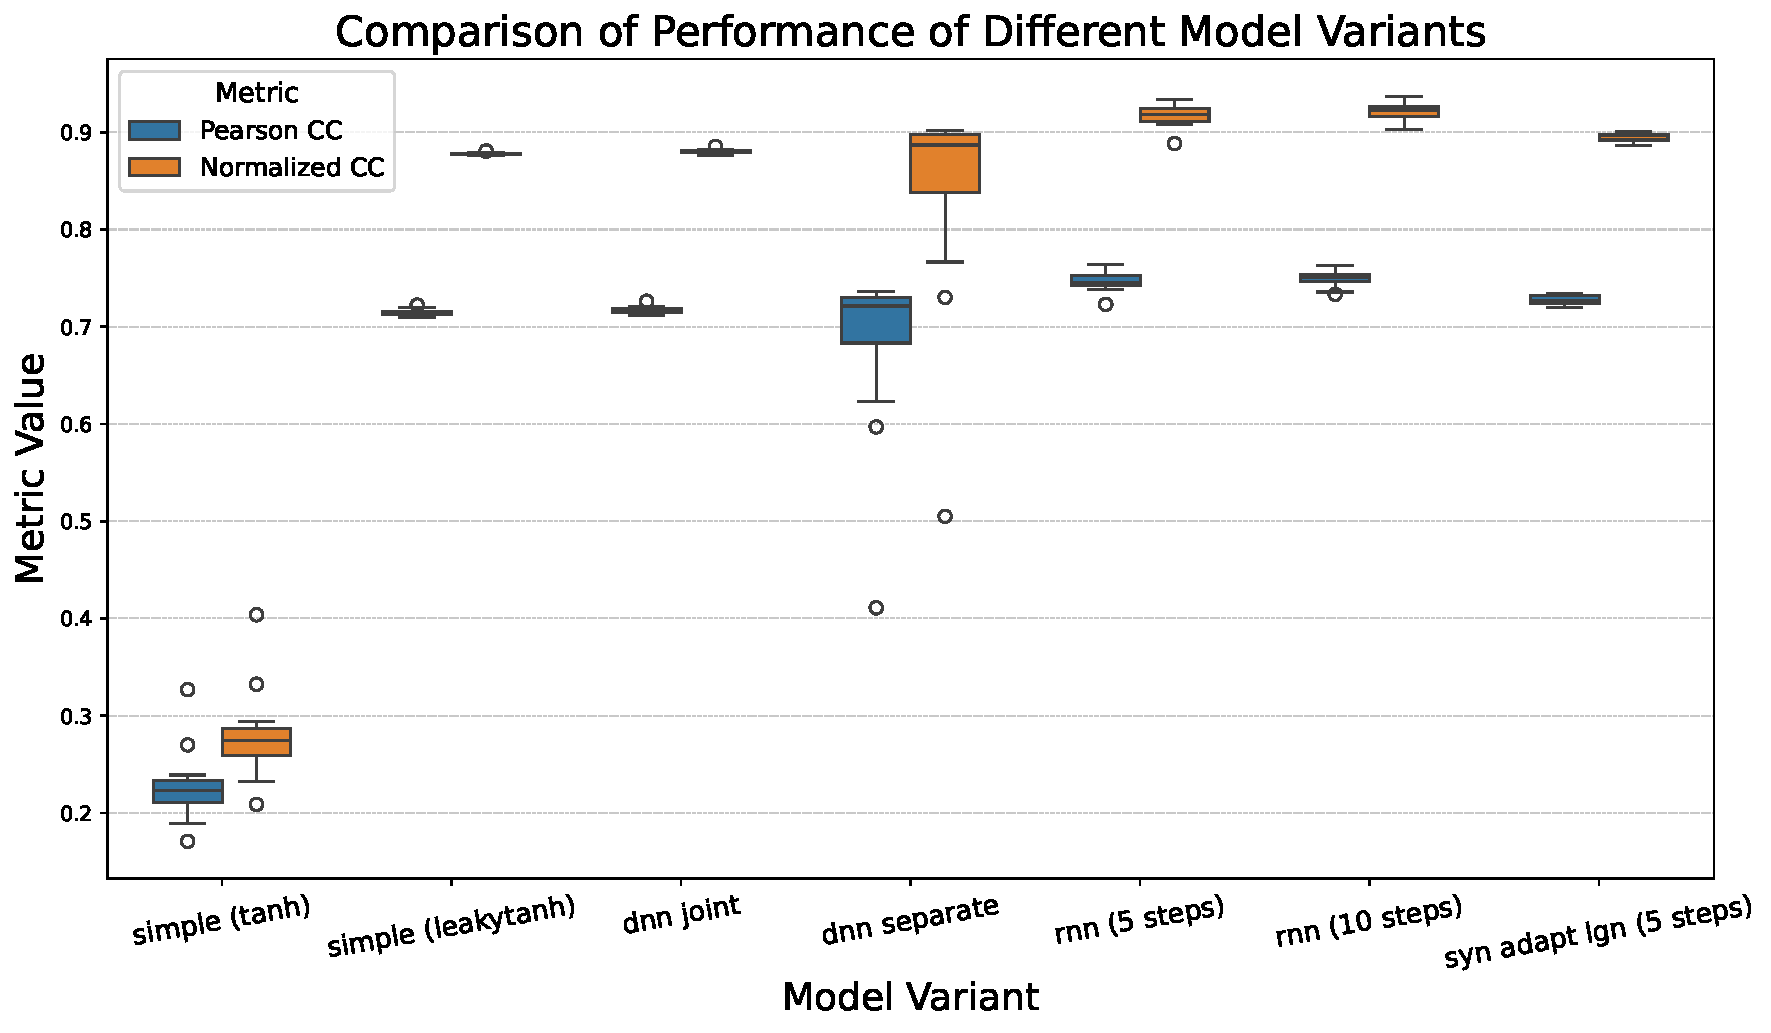
\includegraphics[width=\linewidth]{img/plots/model_types_correlation_comparison.pdf}
    \caption{Boxplot comparing the distribution of Pearson and normalized cross-correlation values across all model variants.}
    \label{fig:model_types_correlation_comparison}
\end{figure}

The results indicate that Pearson and normalized cross-correlation metrics exhibit similar behavior, with the primary difference being a consistent offset due to the normalization process. Given this similarity, we will primarily use normalized cross-correlation in subsequent analyses unless otherwise noted.

One clear outlier in performance is the simple (tanh) model, which significantly underperforms compared to all other models. In contrast, the simple (leakytanh) model, utilizing out custom task-specific activation function, performs comparably to the dnn joint and dnn separate models. This indicates that a well-designed activation function can approximate the functionality of more complex feed-forward modules.

The RNN-based models (rnn (5 steps), rnn (10 steps) and syn adapt lgn (5 steps)) demonstrate superior performance, highlighting the importance of incorporating memory through recurrent structures and TBPTT training. This result suggests that temporal dependencies in neuronal activity are better captured by models with memory components.

Another potential reason why the simple and feed-forward models perform reasonably well could be their ability to capture the mean spiking pattern of the neuronal populations. As previously discussed in Section~\ref{subsec:deep_learning_approach}. The predicted responses are relatively sparse, and high correlation values may partly reflect this sparsity rather than true predictive accuracy. In contrast, the improved performance observed in TBPTT-based models may reflect their enhanced ability to model temporal dynamics in neuronal activity.

Interestingly, the dnn separate model exhibits a high degree of variability across subsets, which is unexpected. Although designed to separate excitatory and inhibitory processing and initially showed results similar to dnn joint during development, its inconsistency may be due to the limited number of subsets (20), or it could reflect limitations in the model architecture when dealing with separate pathways. Additional experiments with a larger number of subsets would be needed to draw firmer conclusions.

The top-performing model overall is rnn (10 steps), which achieves the highest mean normalized correlation and maintains consistent performance across subsets. Increasing the number of TBPTT steps appears beneficial, though further increases were limited by computational constraints.

An unexpected observation is that the syn adapt lgn (5 steps) model underperforms compared to rnn neuron module variants without synaptic depression. This may be due to suboptimal hyperparameter tuning and insufficient number of TBPTT steps, which were not fully explored due to resource limitations.

Finally, we analyze the population spike count patterns of model predictions by comparing their \emph{temporal spiking dynamics curves}, which represent the fraction of simultaneously spiking neurons at each time step (see Section~\ref{subsubsec:neuron_synchrony_binning}). Figure~\ref{fig:boxplot_models_overall_synchrony_pearson_comparison} shows the distribution of Pearson correlation coefficients for both overall predictions and temporal spiking dynamics curves. Note that simple (tanh) is excluded due to technical issues during evaluation.

\begin{figure}
    \centering
    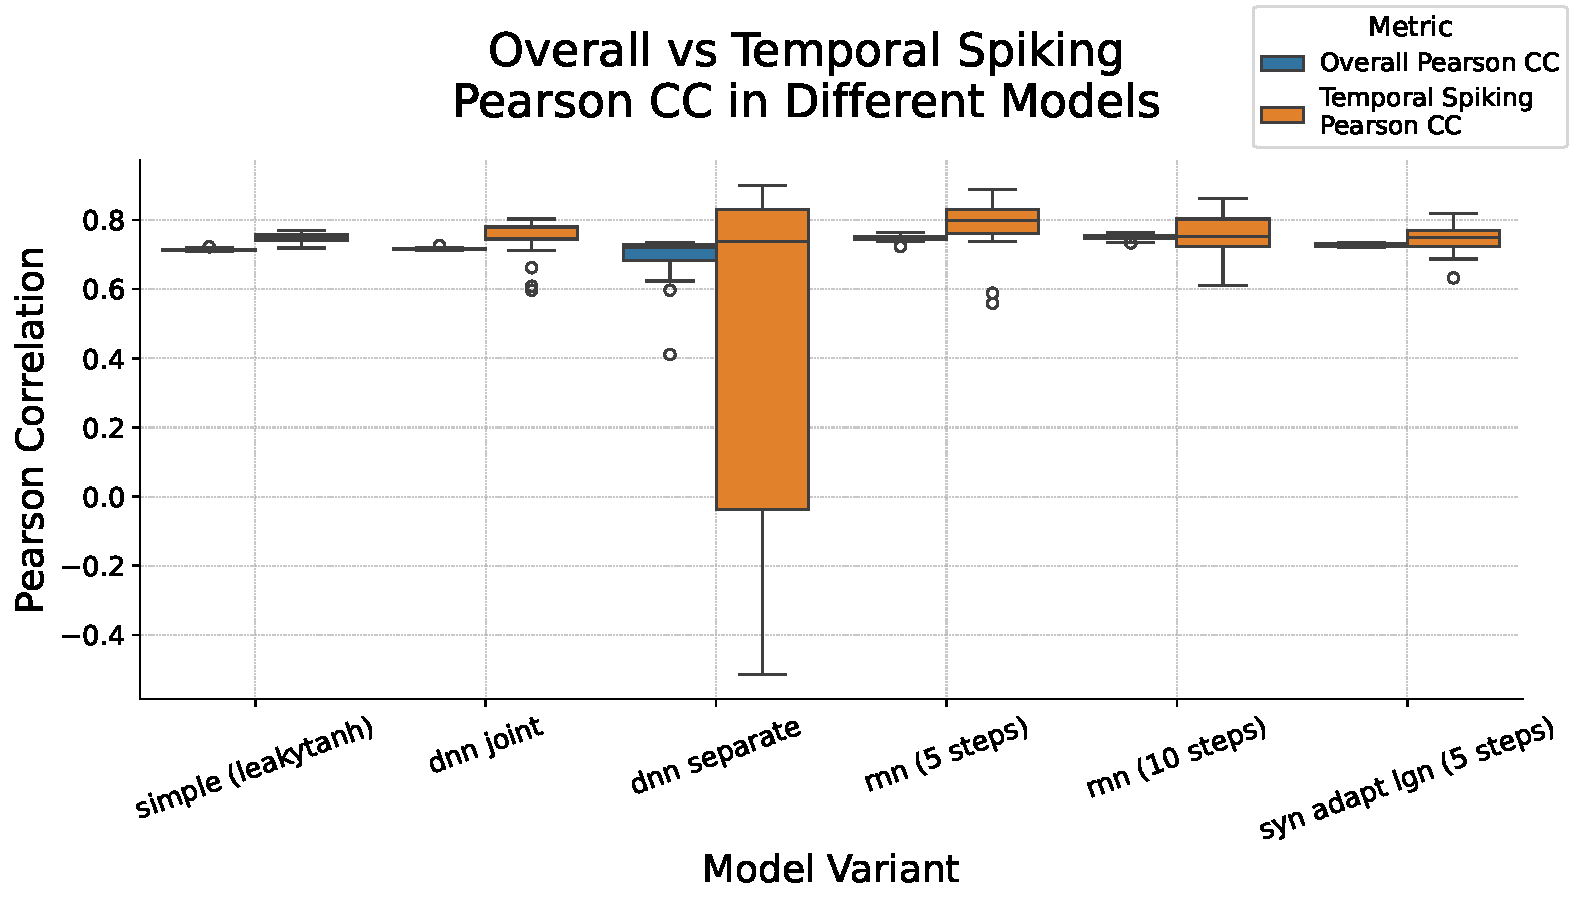
\includegraphics[width=\linewidth]{img/plots/boxplot_model_comparison_synchrony_overall_pearson.pdf}
    \caption{Boxplot comparing Pearson correlation coefficients for model predictions and temporal spiking dynamics curves across all layers and model subsets.}
    \label{fig:boxplot_models_overall_synchrony_pearson_comparison}
\end{figure}

The variance in population spike count correlations is higher than in overall predictions for all models, particularly those trained with TBPTT. We hypothesize it is because these models better capture temporal dynamics. Notably, rnn (5 steps) slightly outperforms rnn (10 steps) in this metric, although this may be an artifact of limited subset size.

The dnn separate model again displays irregular behavior with wide variability in population spike count correlation. This could be due to its architecture, which might struggle with modeling complex input dynamics without memory, or due to technical issues that were not detected. Additional investigation with a more comprehensive dataset is necessary to confirm these findings.

\subsection{Temporal Dynamics of Predicted vs. Actual Neural Activity}
\label{subsec:prediction_target_comparison_variants}

This section focuses on evaluating the temporal behavior of the model predictions. Specifically, we examine the temporal spiking dynamics curves of individual model variants and compare them with the corresponding target temporal spiking dynamics curves. Due to unresolved technical issues during evaluation, the simple (tanh) model is excluded from this analysis, as its predictions could not be retrieved. However, given that the simple (tanh) model has already been shown to perform significantly worse than other models, its exclusion is not expected to compromise the validity of our conclusions.

The primary motivation behind analyzing temporal spiking dynamics curves is to assess whether the models can capture temporal patterns in neuronal activity, an essential aspect of biological realism. Accurate modeling of such dynamics would represent a meaningful advancement over traditional neural network approaches to system identification, as previously discussed in Section~\ref{subsec:deep_learning_approach}.

\subsubsection{Simple Model}
\label{{subsubsec:simpl_leakytanh_eval}}

Figure~\ref{fig:synchrony_curve_simple_leaky_tanh} shows the mean temporal spiking dynamics curve for the simple (leakytanh) model, alongside the target temporal spiking dynamics curve, aggregated across all trials and model subset variants.

\begin{figure}
    \centering
    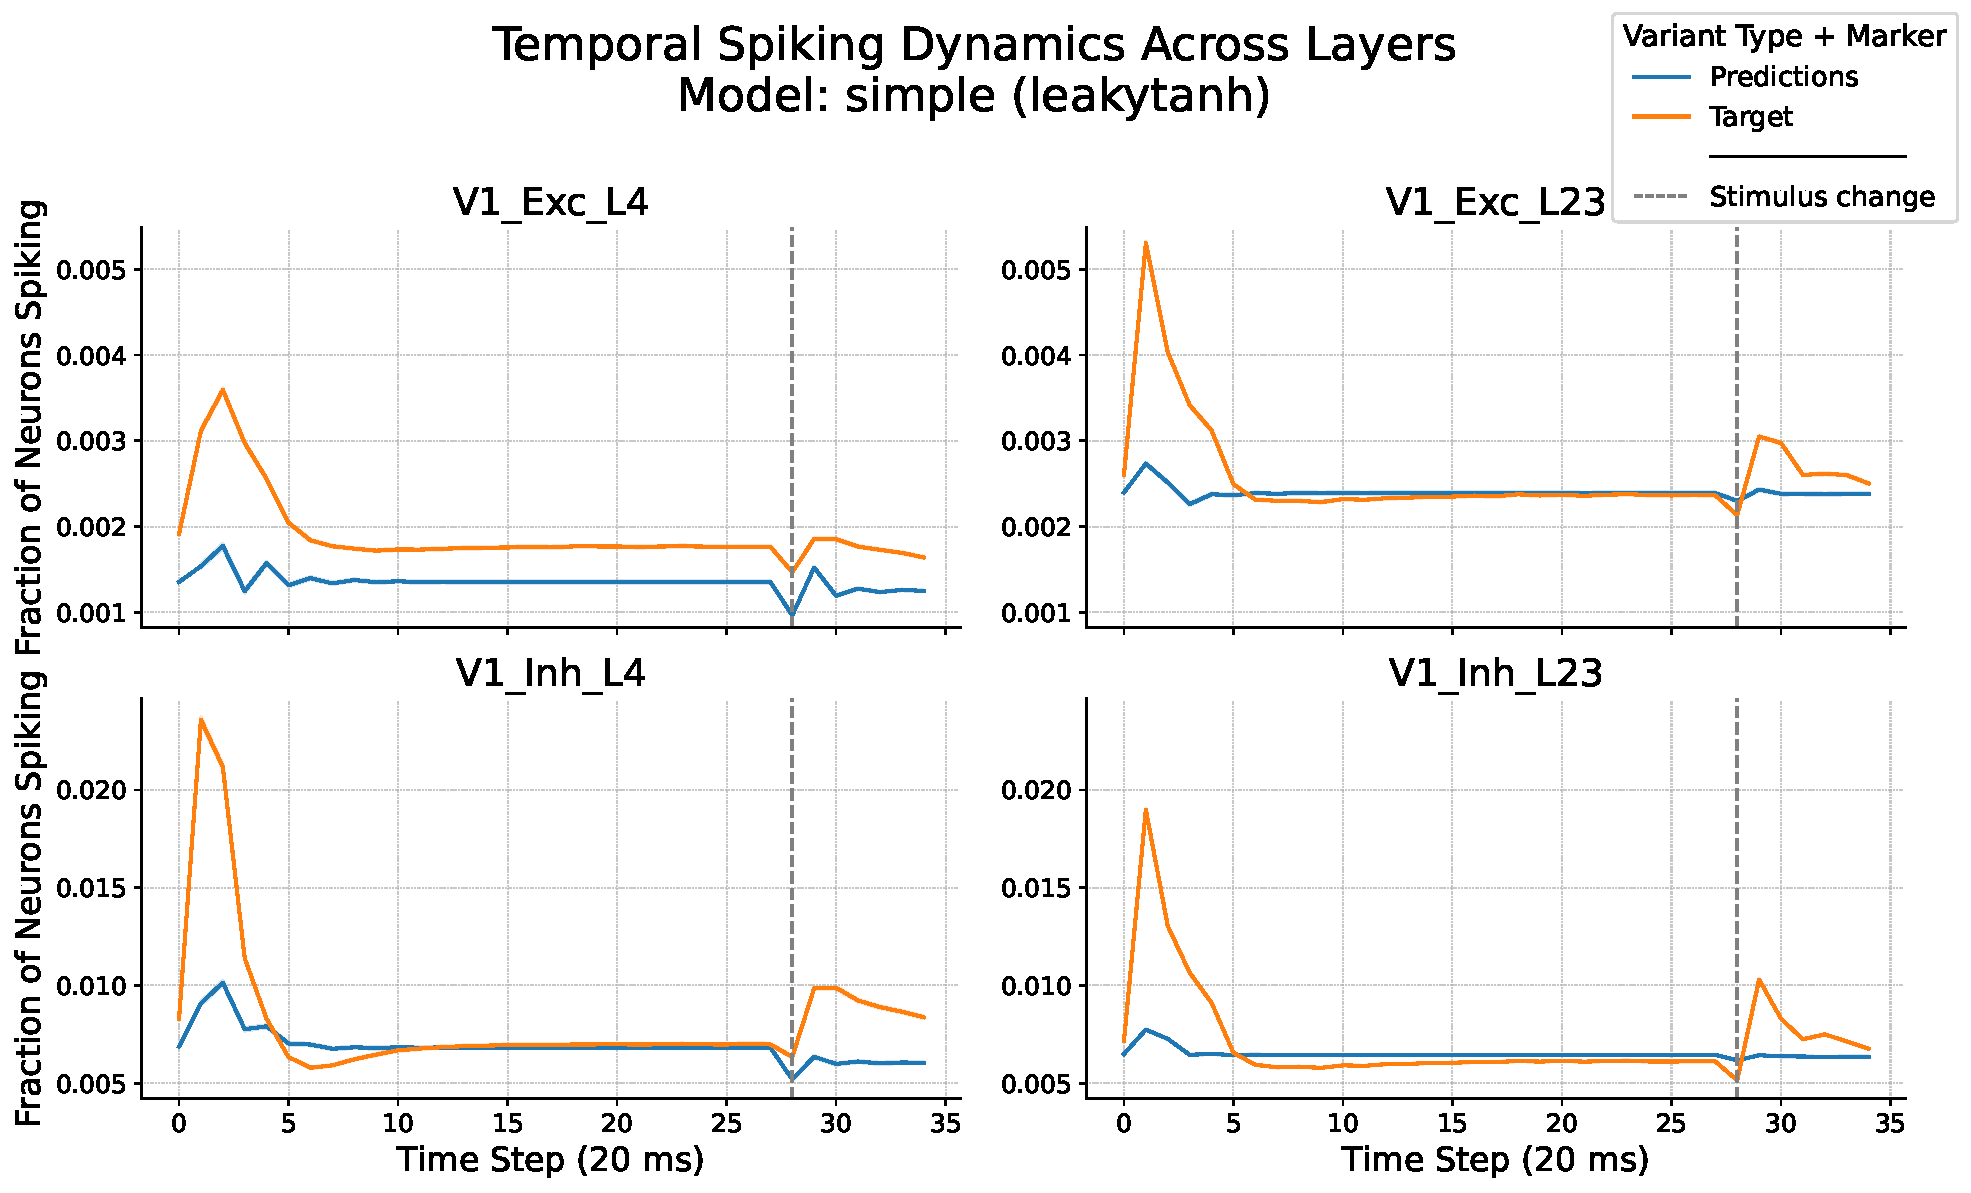
\includegraphics[width=\linewidth]{img/plots/separate_model_synchrony_curve_simple_evaluation_new.pdf}
    \caption{Mean temporal spiking dynamics curve of the simple (leakytanh) model predictions compared to the target temporal spiking dynamics curve. Results are averaged over all trials and model subsets. Error bars represent standard deviation. The dashed vertical line marks the transition from natural to blank stimuli.}
    \label{fig:synchrony_curve_simple_leaky_tanh}
\end{figure}

The temporal spiking dynamics curve for the simple (leakytanh) model exhibits relatively flat behavior across time, suggesting that the model is primarily capturing the mean spiking rate rather than dynamic temporal fluctuations. This behavior results in reasonably accurate predictions during the later phase of stimulus presentation but fails to account for the initial spike in activity during the onset of natural stimuli.

Interestingly, the model successfully captures the decline in population spike count following the switch to blank stimuli, performing reasonably well in comparison to more complex models in this regard.

We hypothesize that the relatively strong performance in capturing average activity levels is due to the use of the specially designed leakytanh activation function. This function constrains predictions within a biologically plausible range, encouraging outputs that align with the mean neuronal response. This interpretation is further supported by the poor performance of the simple (tanh) model, which lacks this task-specific regularization. Although temporal spiking dynamics curve data for the tanh variant are unavailable, its previously reported low correlation values suggest inferior temporal modeling compared to the leakytanh version.


\subsubsection{Feed-Forward Neuronal Module Variants}
\label{{subsubsec:dnn_eval}}
In this section, we examine the temporal spiking dynamics curves of the dnn joint and dnn separate models. Figure~\ref{fig:synchrony_curve_dnn_joint} presents the results for the dnn joint model, while Figure~\ref{fig:synchrony_curve_dnn_separate} displays those for the dnn separate model.
\begin{figure}
    \centering
    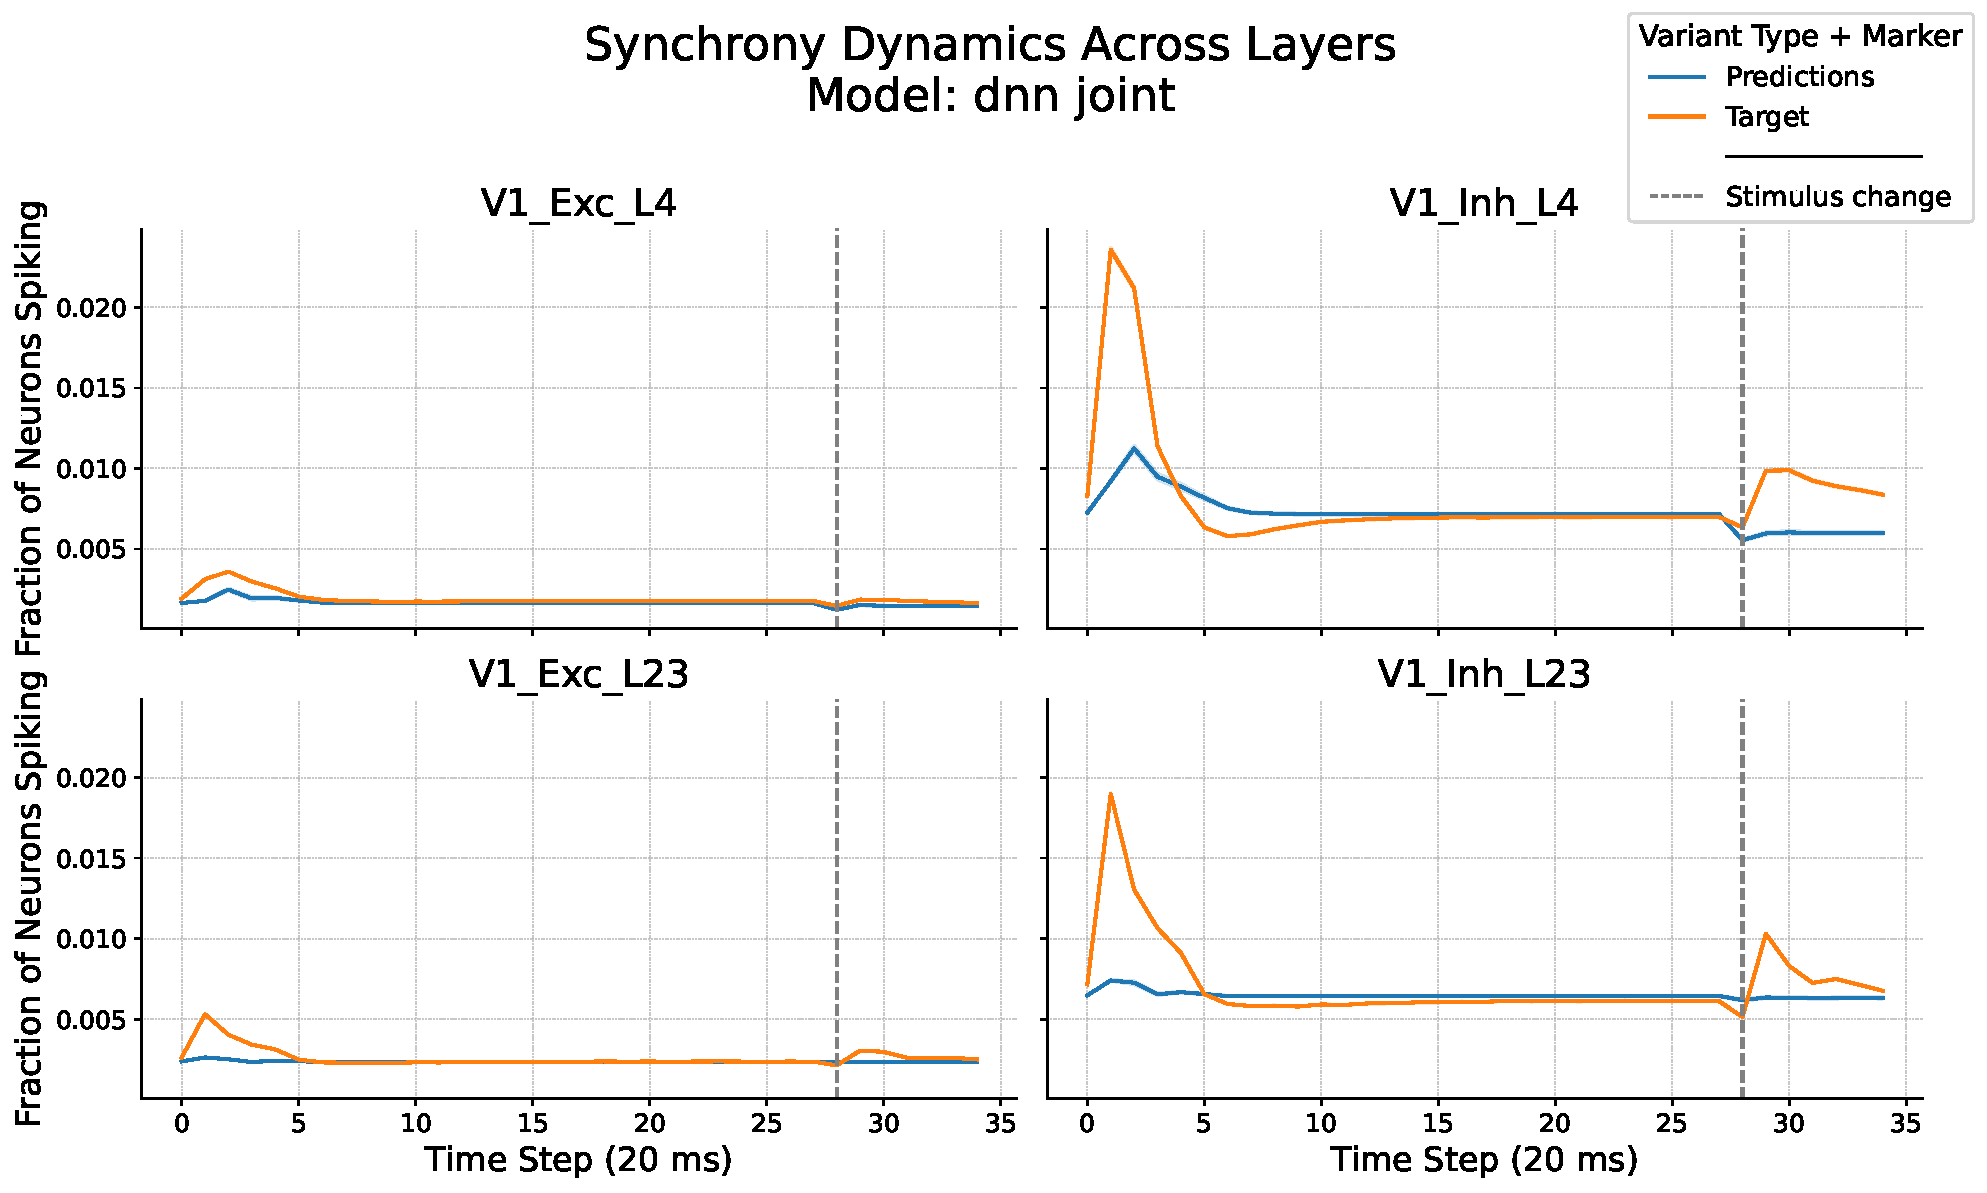
\includegraphics[width=\linewidth]{img/plots/separate_model_synchrony_curve_dnn_joint_evaluation.pdf}
    \caption{Mean temporal spiking dynamics curve of the dnn joint model predictions compared to the target temporal spiking dynamics curve. Results are averaged over all trials and model subsets. Error bars represent standard deviation. The dashed vertical line marks the transition from natural to blank stimuli.}
    \label{fig:synchrony_curve_dnn_joint}
\end{figure}

\begin{figure}
    \centering
    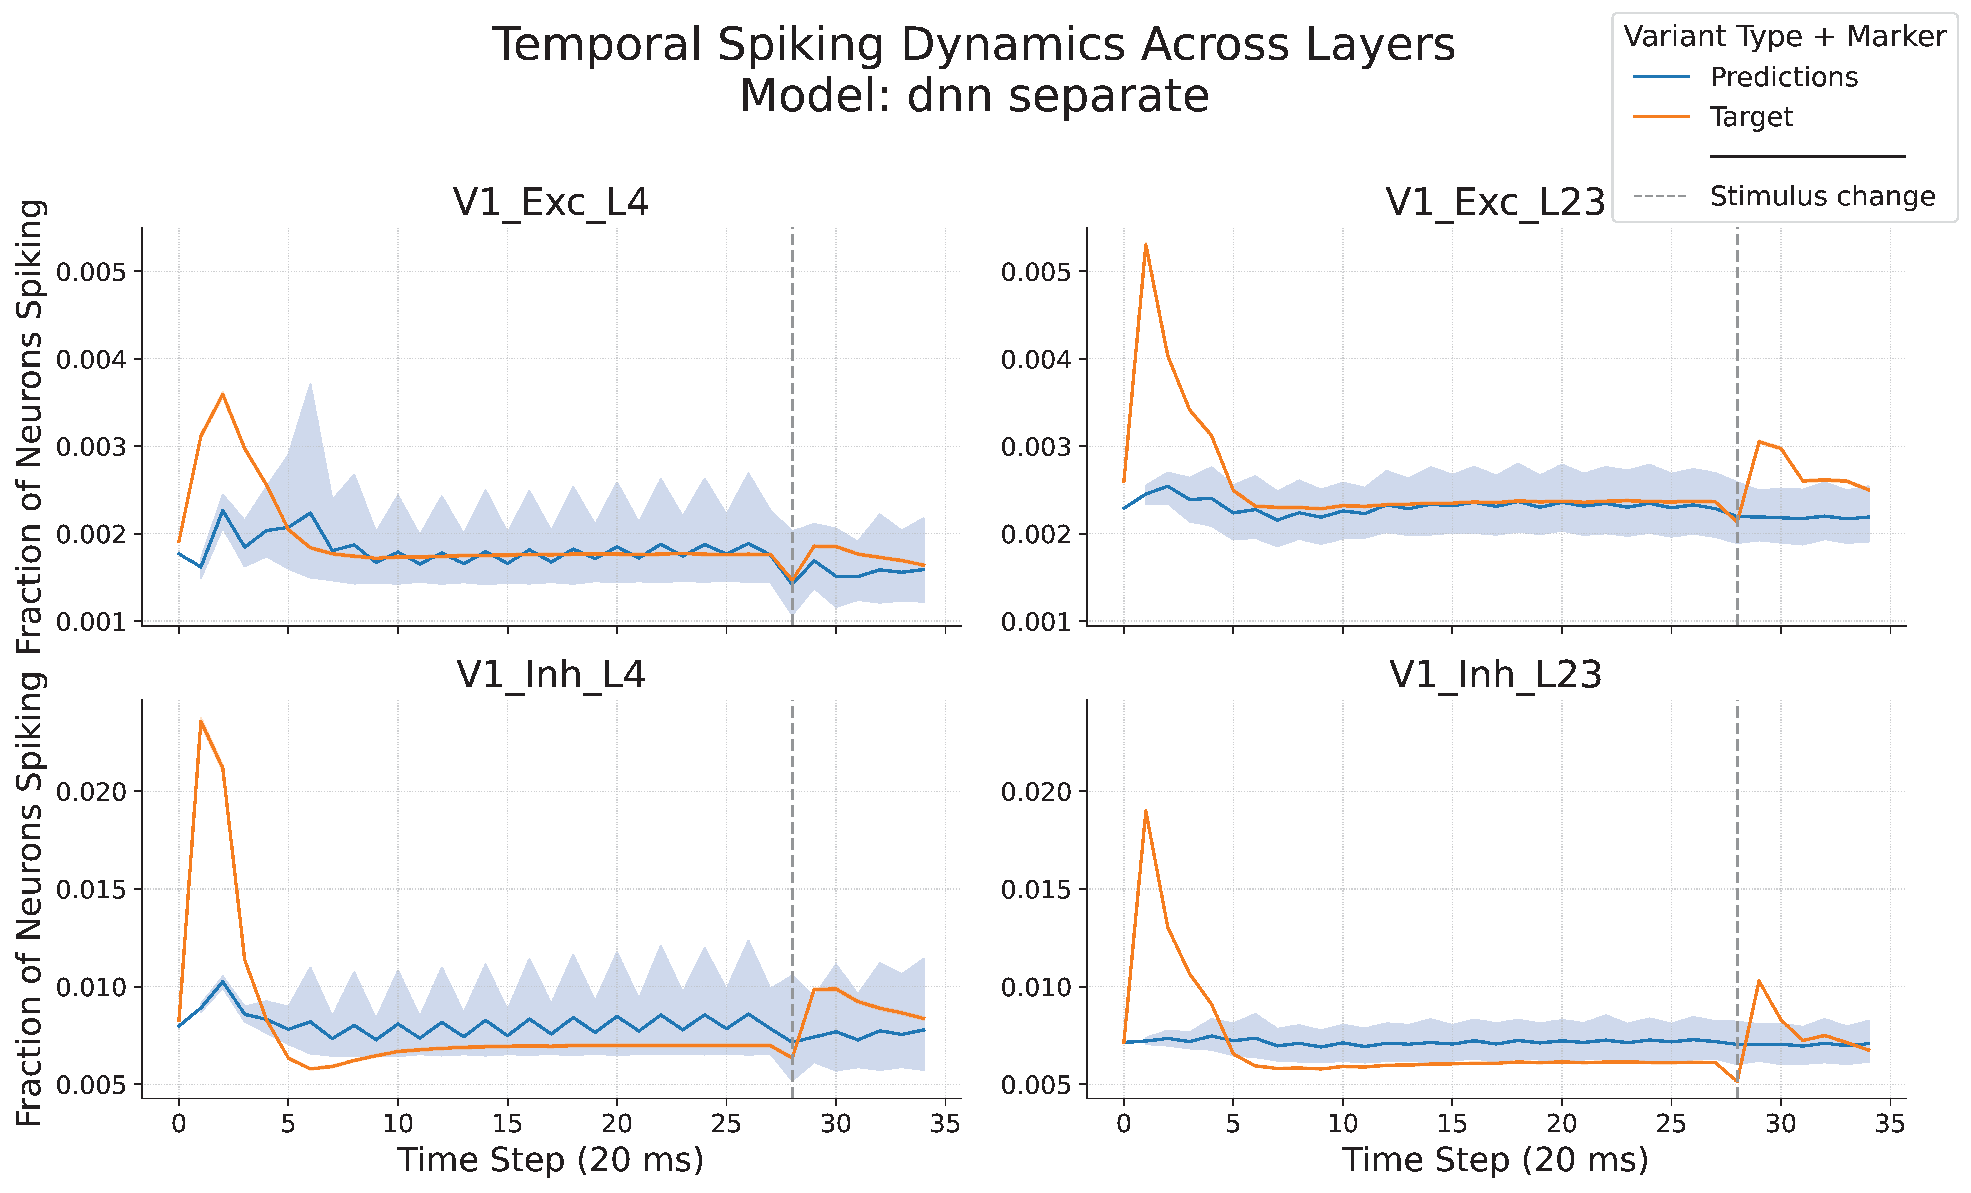
\includegraphics[width=\linewidth]{img/plots/separate_model_synchrony_curve_dnn_separate_evaluation.pdf}
    \caption{Mean temporal spiking dynamics curve of the dnn separate model predictions compared to the target temporal spiking dynamics curve. Results are averaged over all trials and model subsets. Error bars represent standard deviation. The dashed vertical line marks the transition from natural to blank stimuli.}
    \label{fig:synchrony_curve_dnn_separate}
\end{figure}

As previously noted, the dnn separate model exhibits unusually high variability, which is also reflected in the large error margins of its temporal spiking dynamics curve. Since potential explanations for this behavior have already been discussed, we will not revisit this model in detail here.

In contrast, the dnn joint model shows modest improvement in capturing early-stage spiking activity in response to natural stimuli compared to the simple (leakytanh) model. However, the overall pattern remains relatively flat, suggesting that the model continues to prioritize mean spiking activity over dynamic temporal features.

These results suggest that while feed-forward neuron modules may offer a slight enhancement in temporal representation, their lack of internal memory limits their ability to model time-dependent behavior. The observed performance gain is likely attributable to the increased representational capacity of standard feed-forward networks over a fixed activation function like leakytanh. Nonetheless, without mechanisms to retain information about past stimuli, these architectures fall short in accurately modeling temporal dynamics in neuronal activity.

\subsubsection{RNN Neuronal Modules Variants}
\label{{subsubsec:rnn_eval}}

The results from previous model variants naturally lead us to explore the RNN neuronal module variants with the TBPTT (Truncated Backpropagation Through Time) algorithm. TBPTT enables the model to better account for temporal dependencies by allowing gradients to propagate through a defined number of time steps, thereby supporting more accurate modeling of dynamic behaviors in neuronal activity.

Although earlier models incorporate recurrent connections that introduce biological plausibility and support temporal self-modulation, they were trained using a \emph{teacher-forcing} strategy (\citet{NIPS2016_16026d60}). This approach resets the hidden states at each time step using the target neuronal responses, effectively preventing the model from learning temporal patterns across time. In contrast, the RNN variants evaluated in this section maintain hidden states across multiple time steps, enabling the model to learn from the temporal structure during training.

Figures~\ref{fig:synchrony_curve_rnn_5} and~\ref{fig:synchrony_curve_rnn_10} display the temporal spiking dynamics curves for models using RNN neuron modules trained with TBPTT over 5 and 10 time steps, respectively. Both models demonstrate an improvement in capturing temporal dynamics, particularly in the early phase of natural stimulus presentation. This phase is characterized by heightened spiking activity, which the TBPTT models successfully reproduce.

Despite these improvements, a notable limitation remains. The models struggle to accurately capture neuronal responses to blank stimuli. In the model predictions, the population spike count following the transition to the blank phase is comparable to that observed during later stages of the natural stimulus. However, in the target responses, the spiking activity during the blank phase, often referred to as spontaneous neuronal activity (see Section~\ref{subsec:stimulus_sequence}), is notably higher than during prolonged natural stimulus exposure. This discrepancy suggests that the models do not fully account for the suppression of neuronal responses associated with long-term stimulus presentation.

\begin{figure}
    \centering
    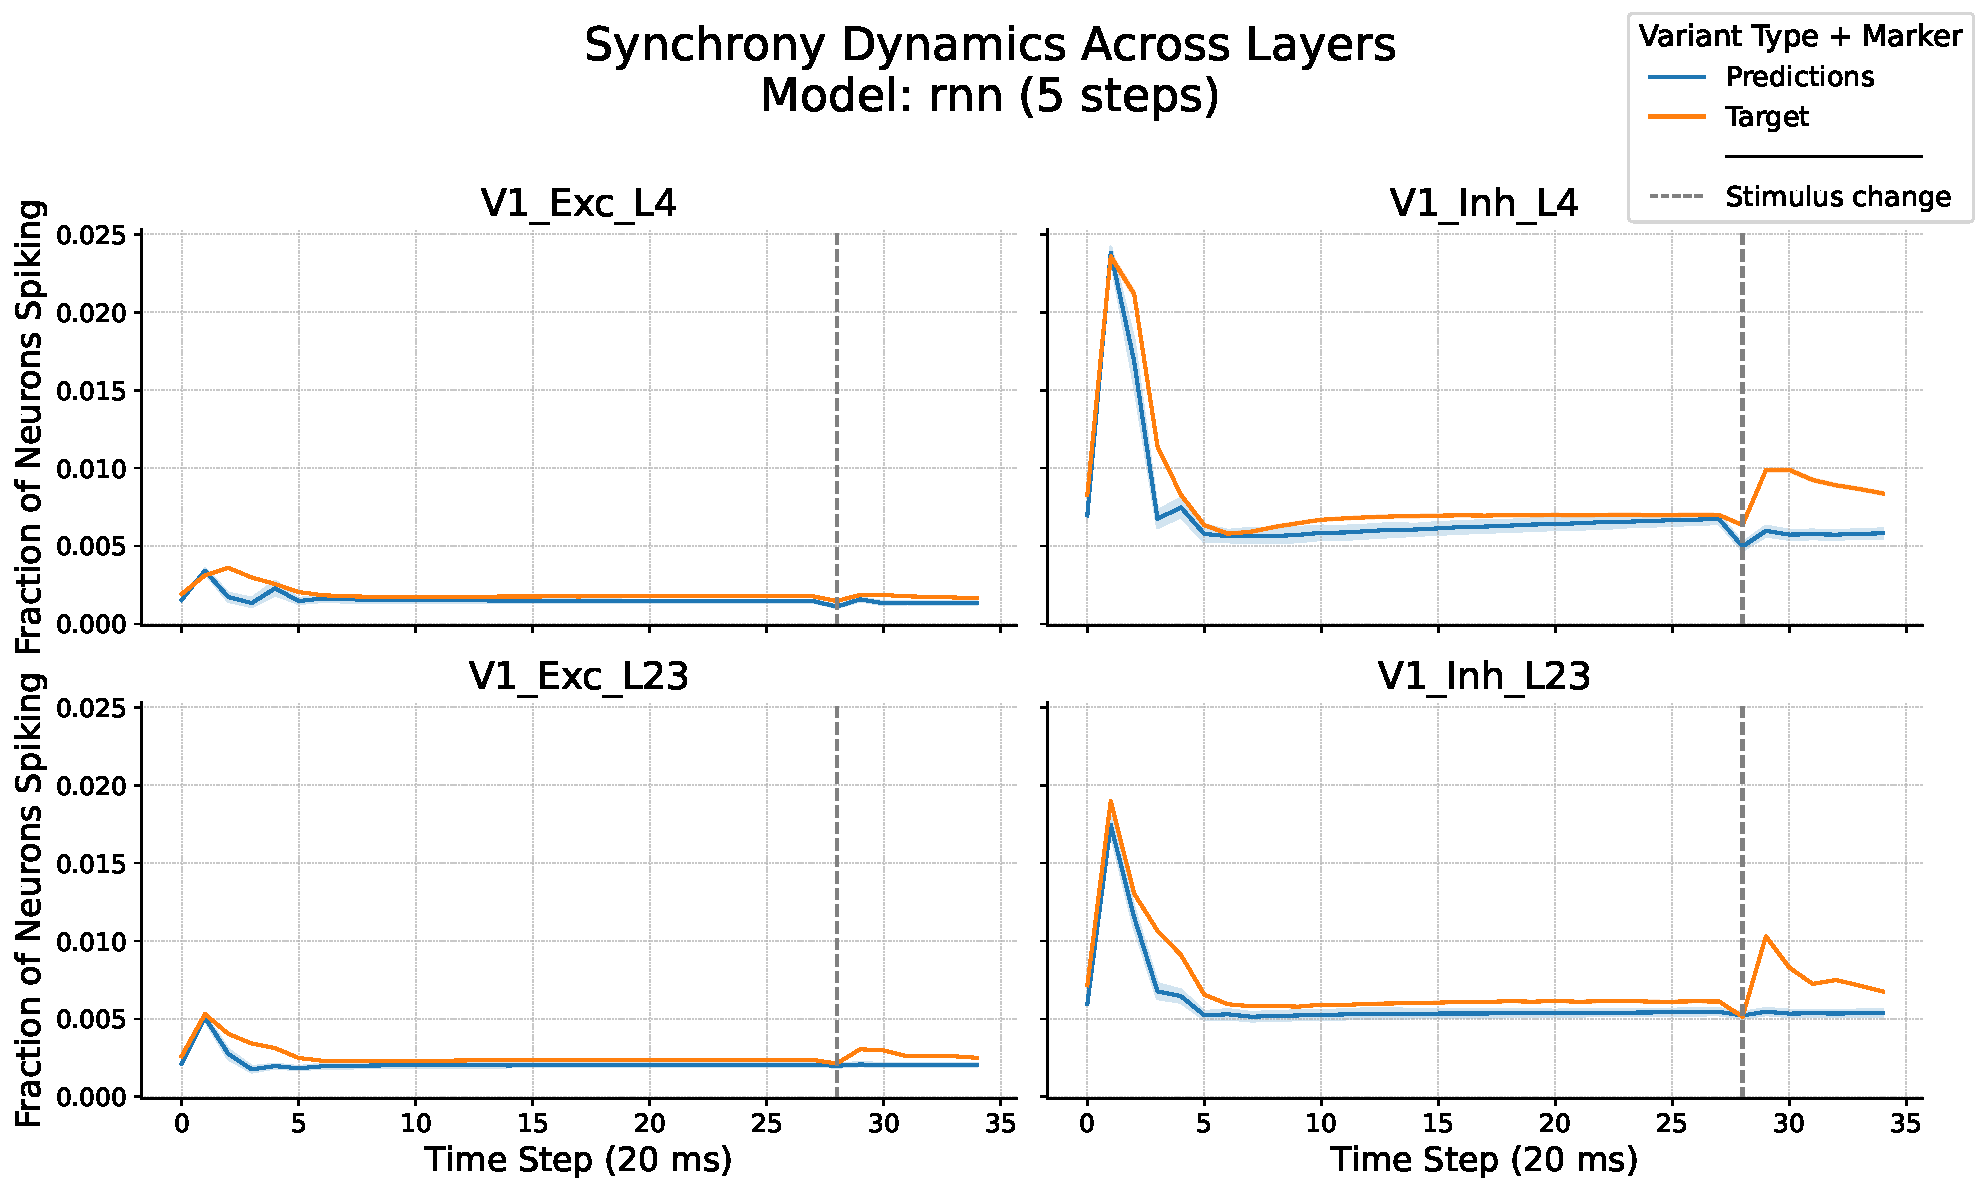
\includegraphics[width=\linewidth]{img/plots/separate_model_synchrony_curve_rnn_separate_5_evaluation.pdf}
    \caption{Mean temporal spiking dynamics curve of the rnn (5 steps) model predictions compared to the target temporal spiking dynamics curve. Results are averaged over all trials and model subsets. Error bars represent standard deviation. The dashed vertical line marks the transition from natural to blank stimuli.}
    \label{fig:synchrony_curve_rnn_5}
\end{figure}

\begin{figure}
    \centering
    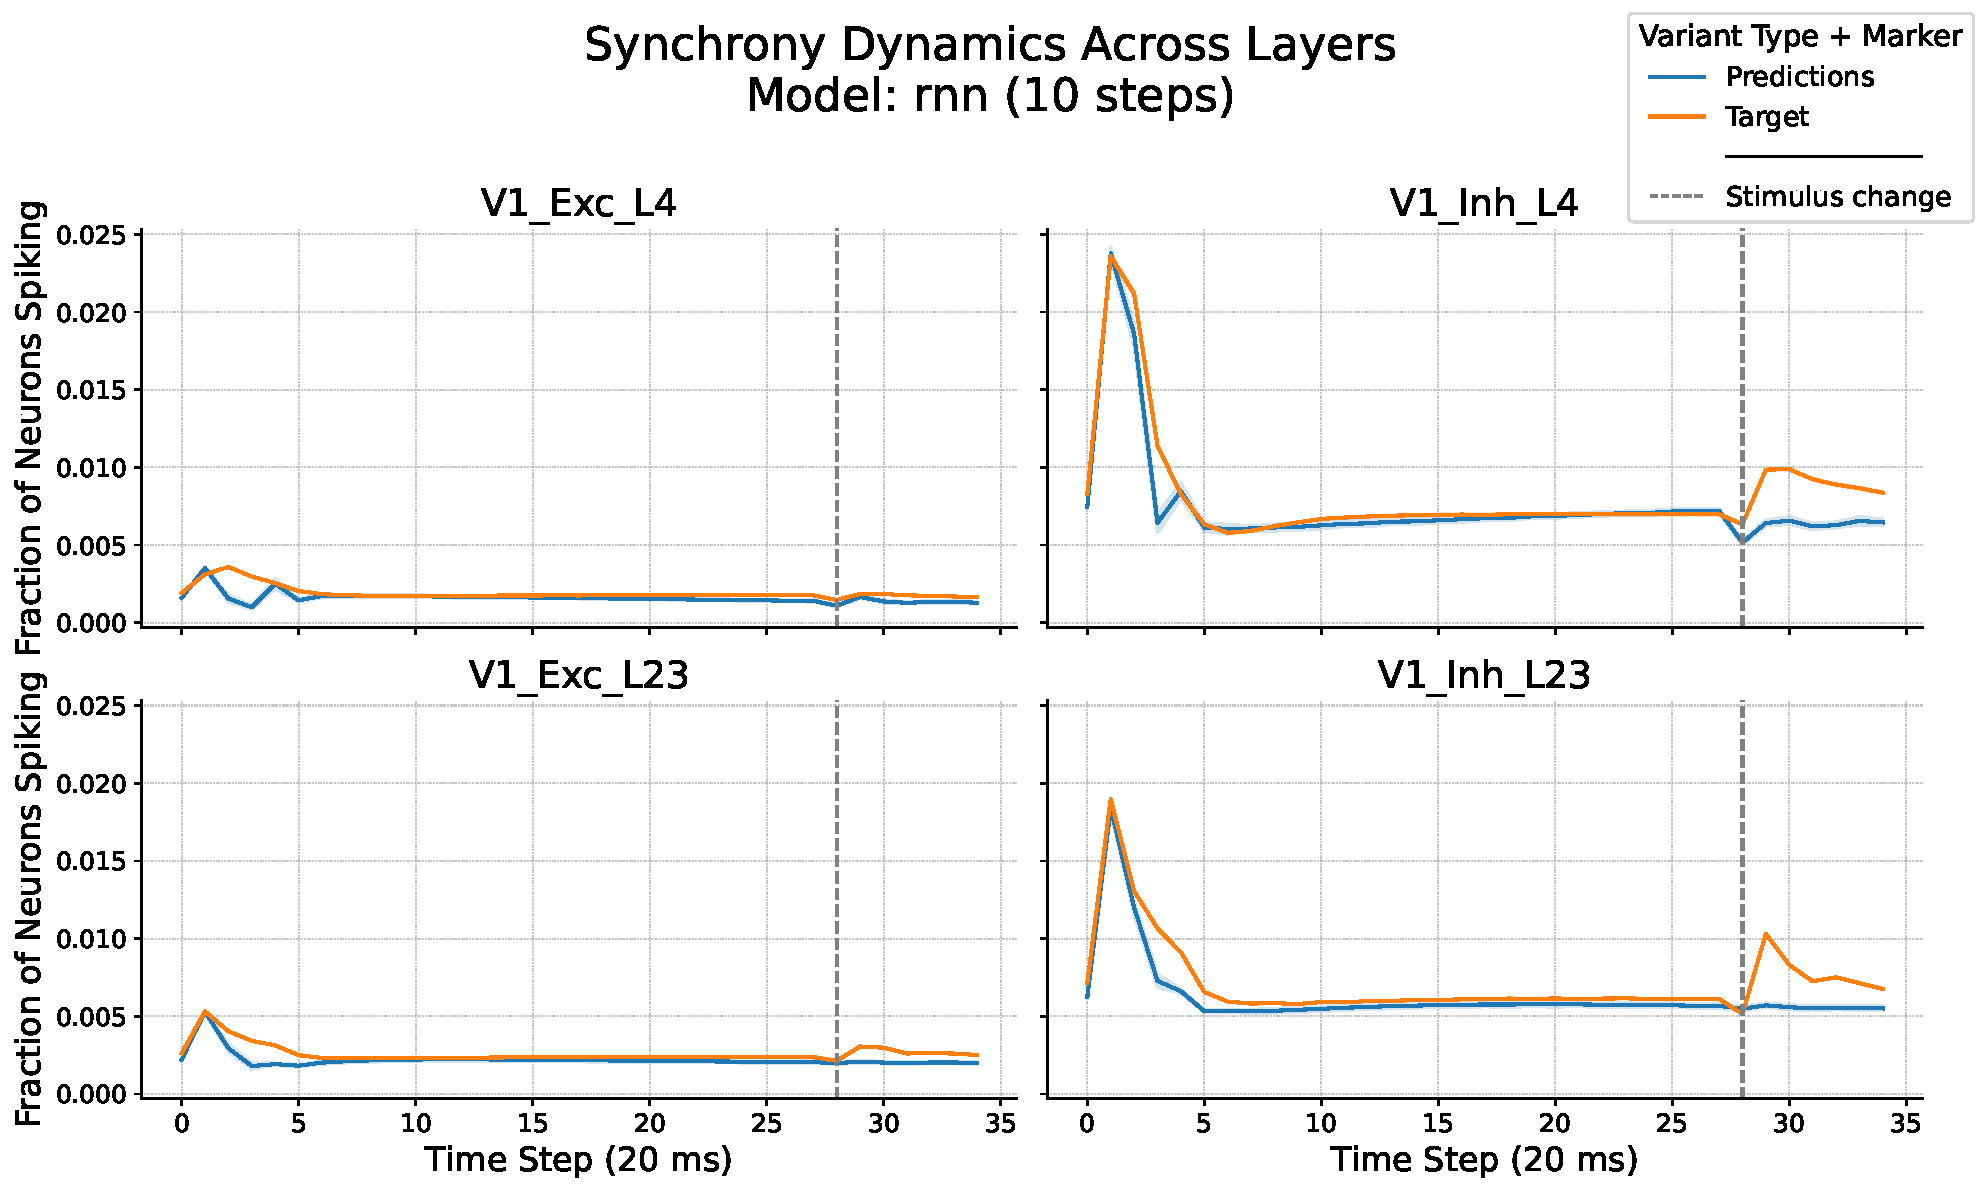
\includegraphics[width=\linewidth]{img/plots/separate_model_synchrony_curve_rnn_separate_10_evaluation.pdf}
    \caption{Mean temporal spiking dynamics curve of the rnn (10 steps) model predictions compared to the target temporal spiking dynamics curve. Results are averaged over all trials and model subsets. Error bars represent standard deviation. The dashed vertical line marks the transition from natural to blank stimuli.}
    \label{fig:synchrony_curve_rnn_10}
\end{figure}

A comparison of the two model variants suggests that increasing the number of TBPTT time steps leads to enhanced model performance. The rnn (10 steps) model not only exhibits more consistent predictions across subset variants but also achieves the highest correlation scores among all tested models, both in normalized and Pearson correlation coefficients.

When reviewing the population spike count-based Pearson correlation coefficients (Figure~\ref{fig:boxplot_models_overall_synchrony_pearson_comparison}), we observe increased variability in TBPTT-trained models relative to their non-TBPTT counterparts. This may be attributed to the greater dynamic range captured by these models. While non-TBPTT models tend to emphasize the stable mean activity, TBPTT models more effectively capture transient dynamics, albeit with slightly less accuracy in static phases.

These findings indicate that models based on RNN neuronal modules trained with TBPTT represent a significant step toward biologically plausible neural network models that can robustly capture temporal patterns. As discussed in Sections~\ref{subsec:deep_learning_approach} and~\ref{subsec:spiking_neural_nets}, the ability to model dynamic neuronal activity is a key criterion for developing interpretable and biologically grounded deep learning systems.

\subsubsection{Synaptic Depression Model}
\label{{subsubsec:syn_adap_lgn_5}}

In the final part of our temporal spiking dynamics curve analysis, we turn to the evaluation of a model incorporating a synaptic depression module. As discussed previously, the temporal dynamics of spontaneous neuronal responses during the blank stimulus phase remain inadequately captured by earlier models. This motivates the integration of synaptic depression mechanisms, which aim to more accurately model the adaptive response of different neuronal populations and improve temporal fidelity.

Experiments with synaptic depression were conducted on a model variant utilizing 5 TBPTT time steps, with the depression mechanism applied specifically to LGN connections. This choice reflects biological evidence indicating that LGN synapses are particularly influenced by synaptic depression. The resulting temporal spiking dynamics curve is shown in Figure~\ref{fig:synchrony_curve_syn_adapt_lgn_5}.

\begin{figure}
    \centering
    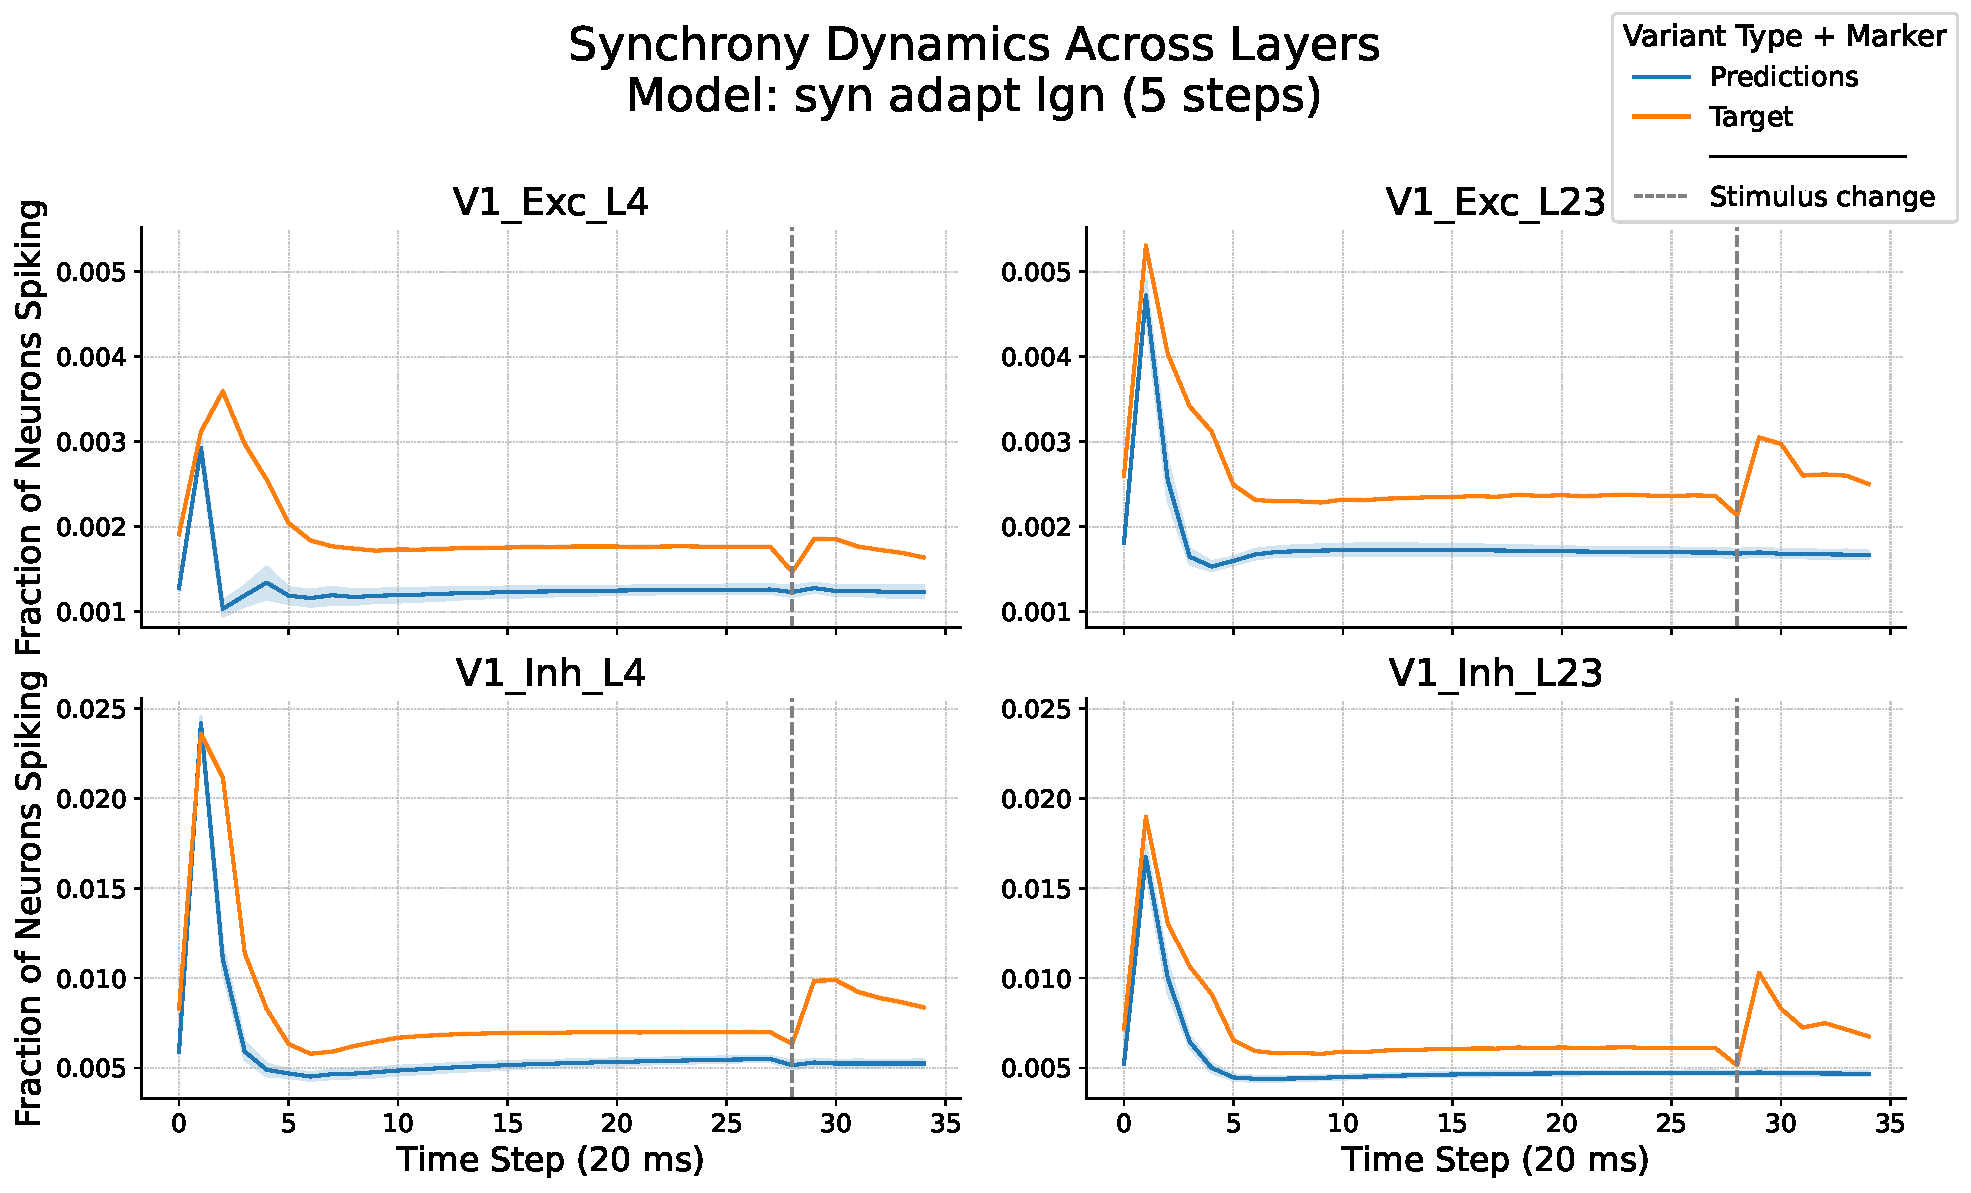
\includegraphics[width=\linewidth]{img/plots/separate_model_synchrony_curve_syn_only_lgn_5_evaluation.pdf}
    \caption{Mean temporal spiking dynamics curve of the syn adapt lgn (5 steps) model predictions compared to the target temporal spiking dynamics curve. Results are averaged over all trials and model subsets. Error bars represent standard deviation. The dashed vertical line marks the transition from natural to blank stimuli.}
    \label{fig:synchrony_curve_syn_adapt_lgn_5}
\end{figure}

This experimental configuration was chosen due to technical constraints. The inclusion of synaptic depression in RNNs dramatically increases memory requirements, especially with longer TBPTT sequences, necessitating high-memory GPU resources. Additionally, training times were significantly extended. As a result, a comprehensive grid search to optimize hyperparameters was not feasible. The hyperparameters used for this model were selected empirically, without the level of tuning applied to other model variants. These limitations likely contributed to the model's suboptimal performance and the inconsistencies observed in its predictions.

The temporal spiking dynamics curve shows that, while the model performs better than non-TBPTT variants, it underperforms relative to RNN models without synaptic depression. Notably, performance appears degraded across the entire stimulus timeline. There is reduced accuracy in modeling the transition from natural to blank stimuli and diminished representation of average neuronal responses in later stages. Furthermore, the model fails to improve prediction of spontaneous responses during the blank phase.

These findings are unexpected, as the incorporation of biologically inspired mechanisms was anticipated to enhance performance. We hypothesize that the underwhelming results are due to the suboptimal hyperparameter configuration and the limited temporal depth (5 TBPTT steps). Additionally, the training dataset may lack sufficient variability to enable the model to generalize dynamic patterns effectively. Further experimentation with improved computational resources and a more diverse dataset may be necessary to fully evaluate the potential of synaptic depression mechanisms in temporal modeling.

\subsection{Statistical Comparison of Model Performance}
\label{subsec:model_performance_statistical_comparison}

To further support our conclusions regarding model performance, we conducted a pairwise one-sided Mann-Whitney U test \citep{mann_whithey_1947}. This non-parametric test was chosen because the underlying distribution of normalized cross-correlation (CC) values for each model is unknown, making parametric tests less appropriate. The one-sided Mann-Whitney U test evaluates whether the distribution of one sample is statistically greater than or equal to another, without assuming a specific distributional form.

We applied this test to all pairwise combinations of model variants, comparing their normalized CC distributions. The results are visualized as a heatmap in Figure~\ref{fig:model_types_p_values_heatmap}, where each cell represents the p-value of a one-sided test. In this visualization, a row model ("Model A") is tested against a column model ("Model B"). A p-value below the significance level $\alpha = 0.05$ indicates that "Model A" significantly outperforms "Model B" in terms of normalized CC.

\begin{figure}
    \centering
    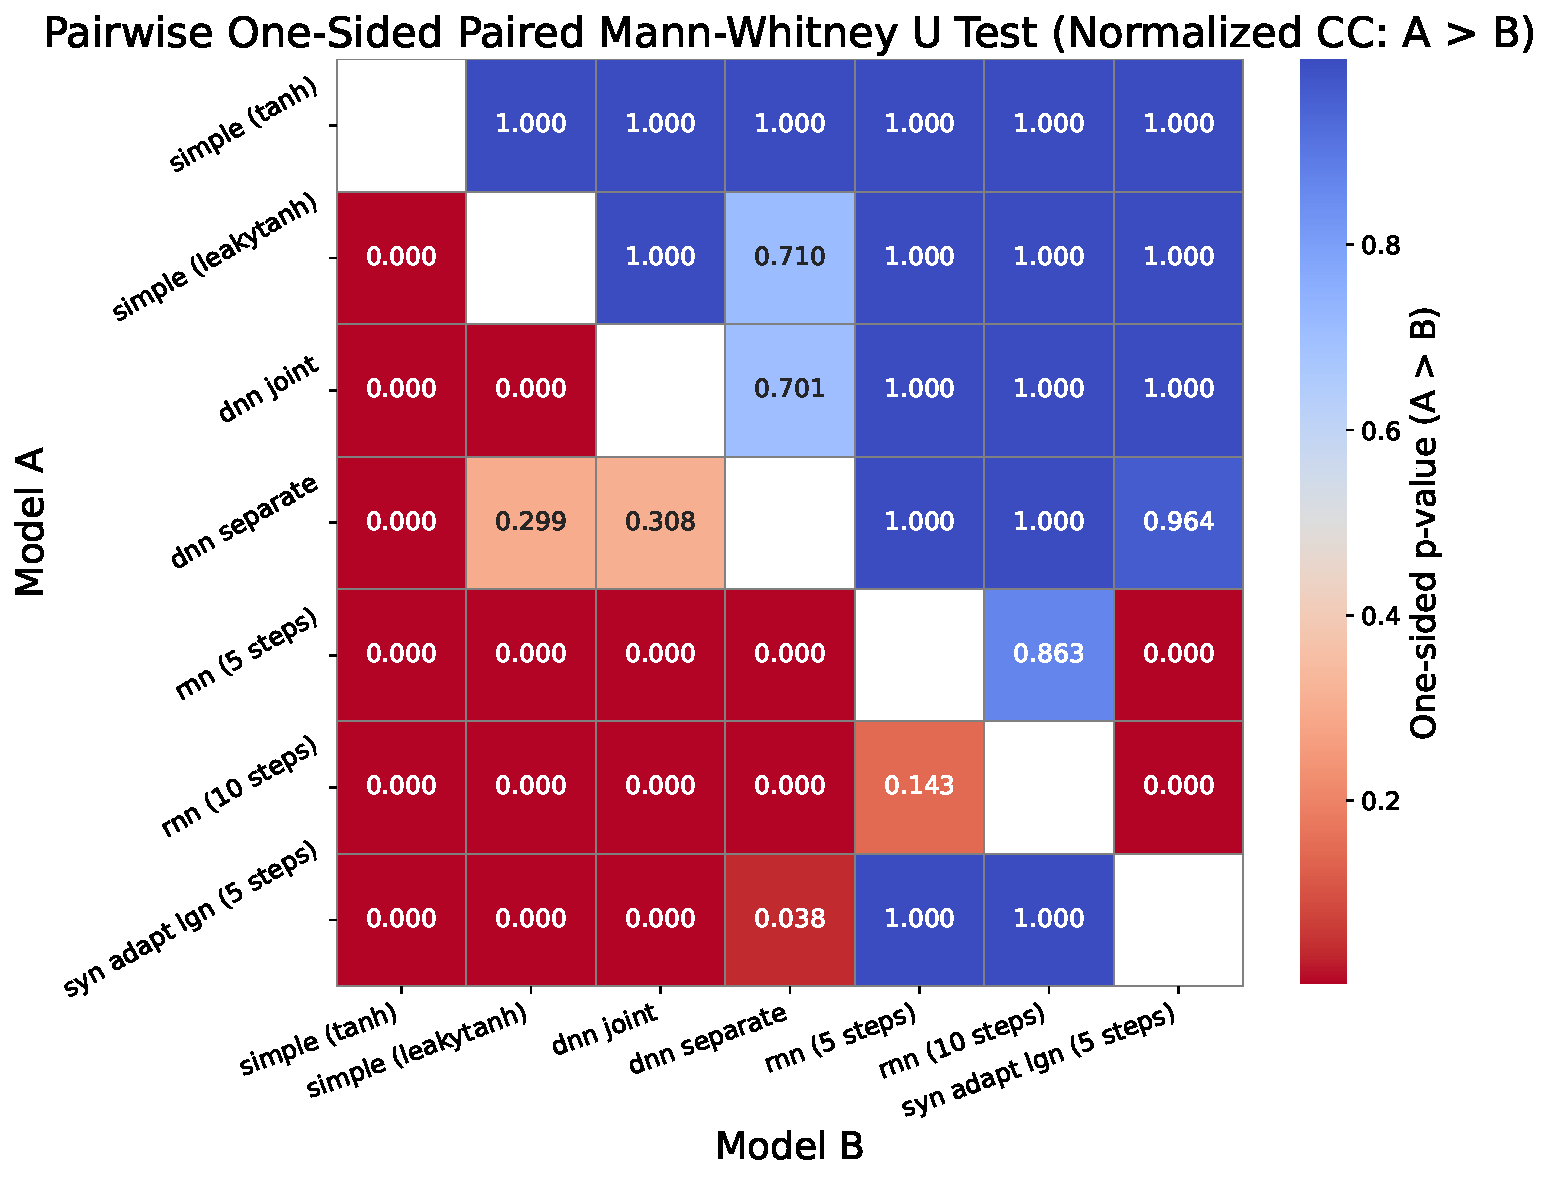
\includegraphics[width=\linewidth]{img/plots/model_types_p_value_heatmap_cc_norm.pdf}
    \caption{Heatmap of p-values from one-sided pairwise Mann-Whitney U tests on normalized cross-correlation values across model variants. Each tile represents a test of whether the row model performs significantly better than the column model. Values below the significance threshold ($\alpha = 0.05$) reject the null hypothesis that both models perform equally or that the row model performs worse.}
    \label{fig:model_types_p_values_heatmap}
\end{figure}

The statistical results largely corroborate the insights obtained from previous visual analyses of mean, variance and population spike count. At the $\alpha = 0.05$ level, we reject the hypothesis that the simple (tanh) model performs better than any other variant, reinforcing its role as the weakest model. Among the more complex models, the results generally support the idea that additional architectural components and biologically inspired features enhance model performance.

However, two models deviate from this trend. The dnn separate model, which has already been noted for its high performance variability, shows inconsistent statistical superiority. Similarly, the syn adapt lgn (5 steps) model underperforms in comparison to RNN neuronal modules models that lack synaptic depression. As previously discussed, this may be attributed to limitations in hyperparameter tuning, dataset diversity, and computational resources.

In summary, the Mann-Whitney U test provides statistical confirmation that, overall, more complex and biologically grounded models tend to perform better. Exceptions to this trend appear to be primarily due to technical and experimental constraints rather than inherent limitations of the model architectures themselves.

\section{Analysis of Model Limitations and Improvement Opportunities}
\label{sec:performace_gaps_and_opportunities_for_improvement}

Up to this point, we have compared various model architectures and concluded that, with the exception of the synaptic depression variant, increasing biological realism generally enhances model performance. Nonetheless, certain shortcomings remain, particularly in capturing the temporal dynamics of spontaneous neuronal activity. In this section, we examine several contributing factors to these performance gaps and explore potential approaches for improvement.

\subsection{Free vs Teacher-Forced Prediction Analysis}
\label{{subsec:free_vs_teacher_forced_predictions}}

We begin by comparing two evaluation strategies: teacher-forced prediction, in which the model's hidden states are reset at each time step using ground truth responses, and free prediction, where the model autonomously generates sequences without external correction. This comparison focuses mainly on the top-performing TBPTT-trained models, which not only yield superior performance but also exhibit a higher degree of biological plausibility.

Figure~\ref{fig:boxplot_models_pearson_synchrony_different_layers} presents the distribution of Pearson correlation coefficients between model predictions and target temporal spiking dynamics curves, separated by layer and prediction mode, excluding the simple (tanh) model.

\begin{figure}
    \centering
    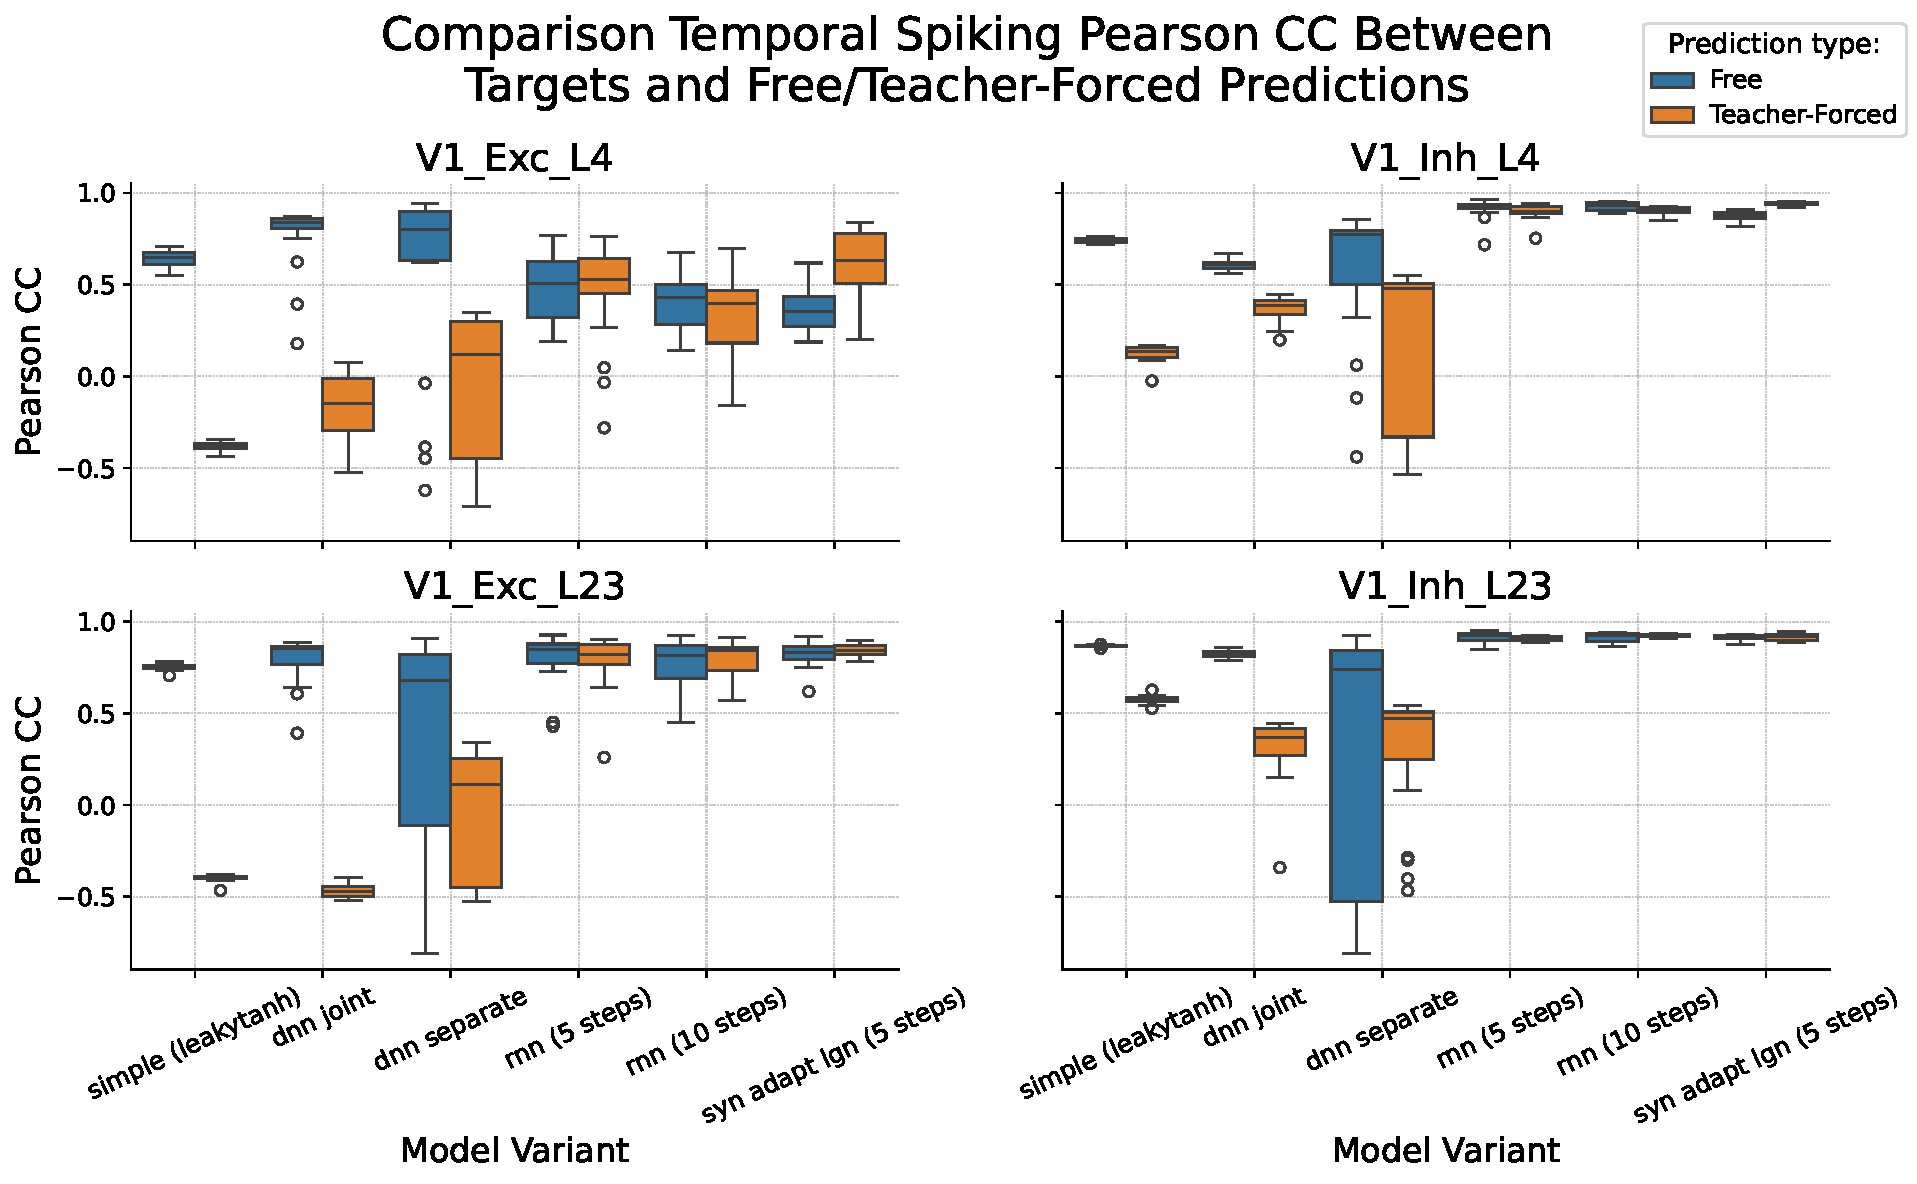
\includegraphics[width=\linewidth]{img/plots/boxplot_model_comparison_synchrony_pearson_layers.pdf}
    \caption{Distribution of Pearson correlation coefficients between predicted and target temporal spiking dynamics curves, shown separately for each layer across all model variants.}
    \label{fig:boxplot_models_pearson_synchrony_different_layers}
\end{figure}

As observed previously, the dnn separate model exhibits inconsistent behavior. Interestingly, performance varies across layer types. TBPTT-trained models consistently outperform others across majority of layers, although their advantage is less significant in excitatory layers. This discrepancy may be attributed to the relatively sparse activity of excitatory neurons. Since non-TBPTT models tend to approximate mean responses well, they may outperform TBPTT models in these layers. In contrast, TBPTT models achieve superior performance in inhibitory layers, which exhibit higher spiking activity.

Another notable observation is that teacher-forced predictions often match or exceed the performance of free predictions in TBPTT models. This result is expected: well-trained TBPTT models should already predict subsequent hidden states with high accuracy, making the teacher-forced reset only a minor adjustment. In some cases, this reset may even improve predictions by initializing the model with more accurate hidden states.

Interestingly, the largest improvement under teacher-forced prediction is seen in the synaptic depression model. This suggests that the model may not be effectively learning temporal dependencies, and that extending the TBPTT horizon or increasing training duration could enhance performance.

Conversely, non-TBPTT models perform worse under teacher-forced evaluation. While one might expect hidden state resets to improve performance, given their similarity to the training procedure, we hypothesize that these resets may disrupt the model's predictions during the high-activity early stimulus phase. Because these models primarily learn mean responses, abrupt resets may distort predictions away from expected averages, resulting in decreased the population spike count CC.


\subsubsection{Teacher-Forced Temporal Spiking Dynamics Curves on TBPTT Model Variants}
\label{subsubsec:teacher_forced_synchrony_curves_tbptt}
In this section, we narrow our focus to the TBPTT-trained model variants. We compare their temporal spiking dynamics curves under both free prediction and teacher-forced prediction modes, alongside the target temporal spiking dynamics curves. This comparison is illustrated in Figure~\ref{fig:free_vs_teacher_forced_synchrony}.

\begin{figure}
    \centering
    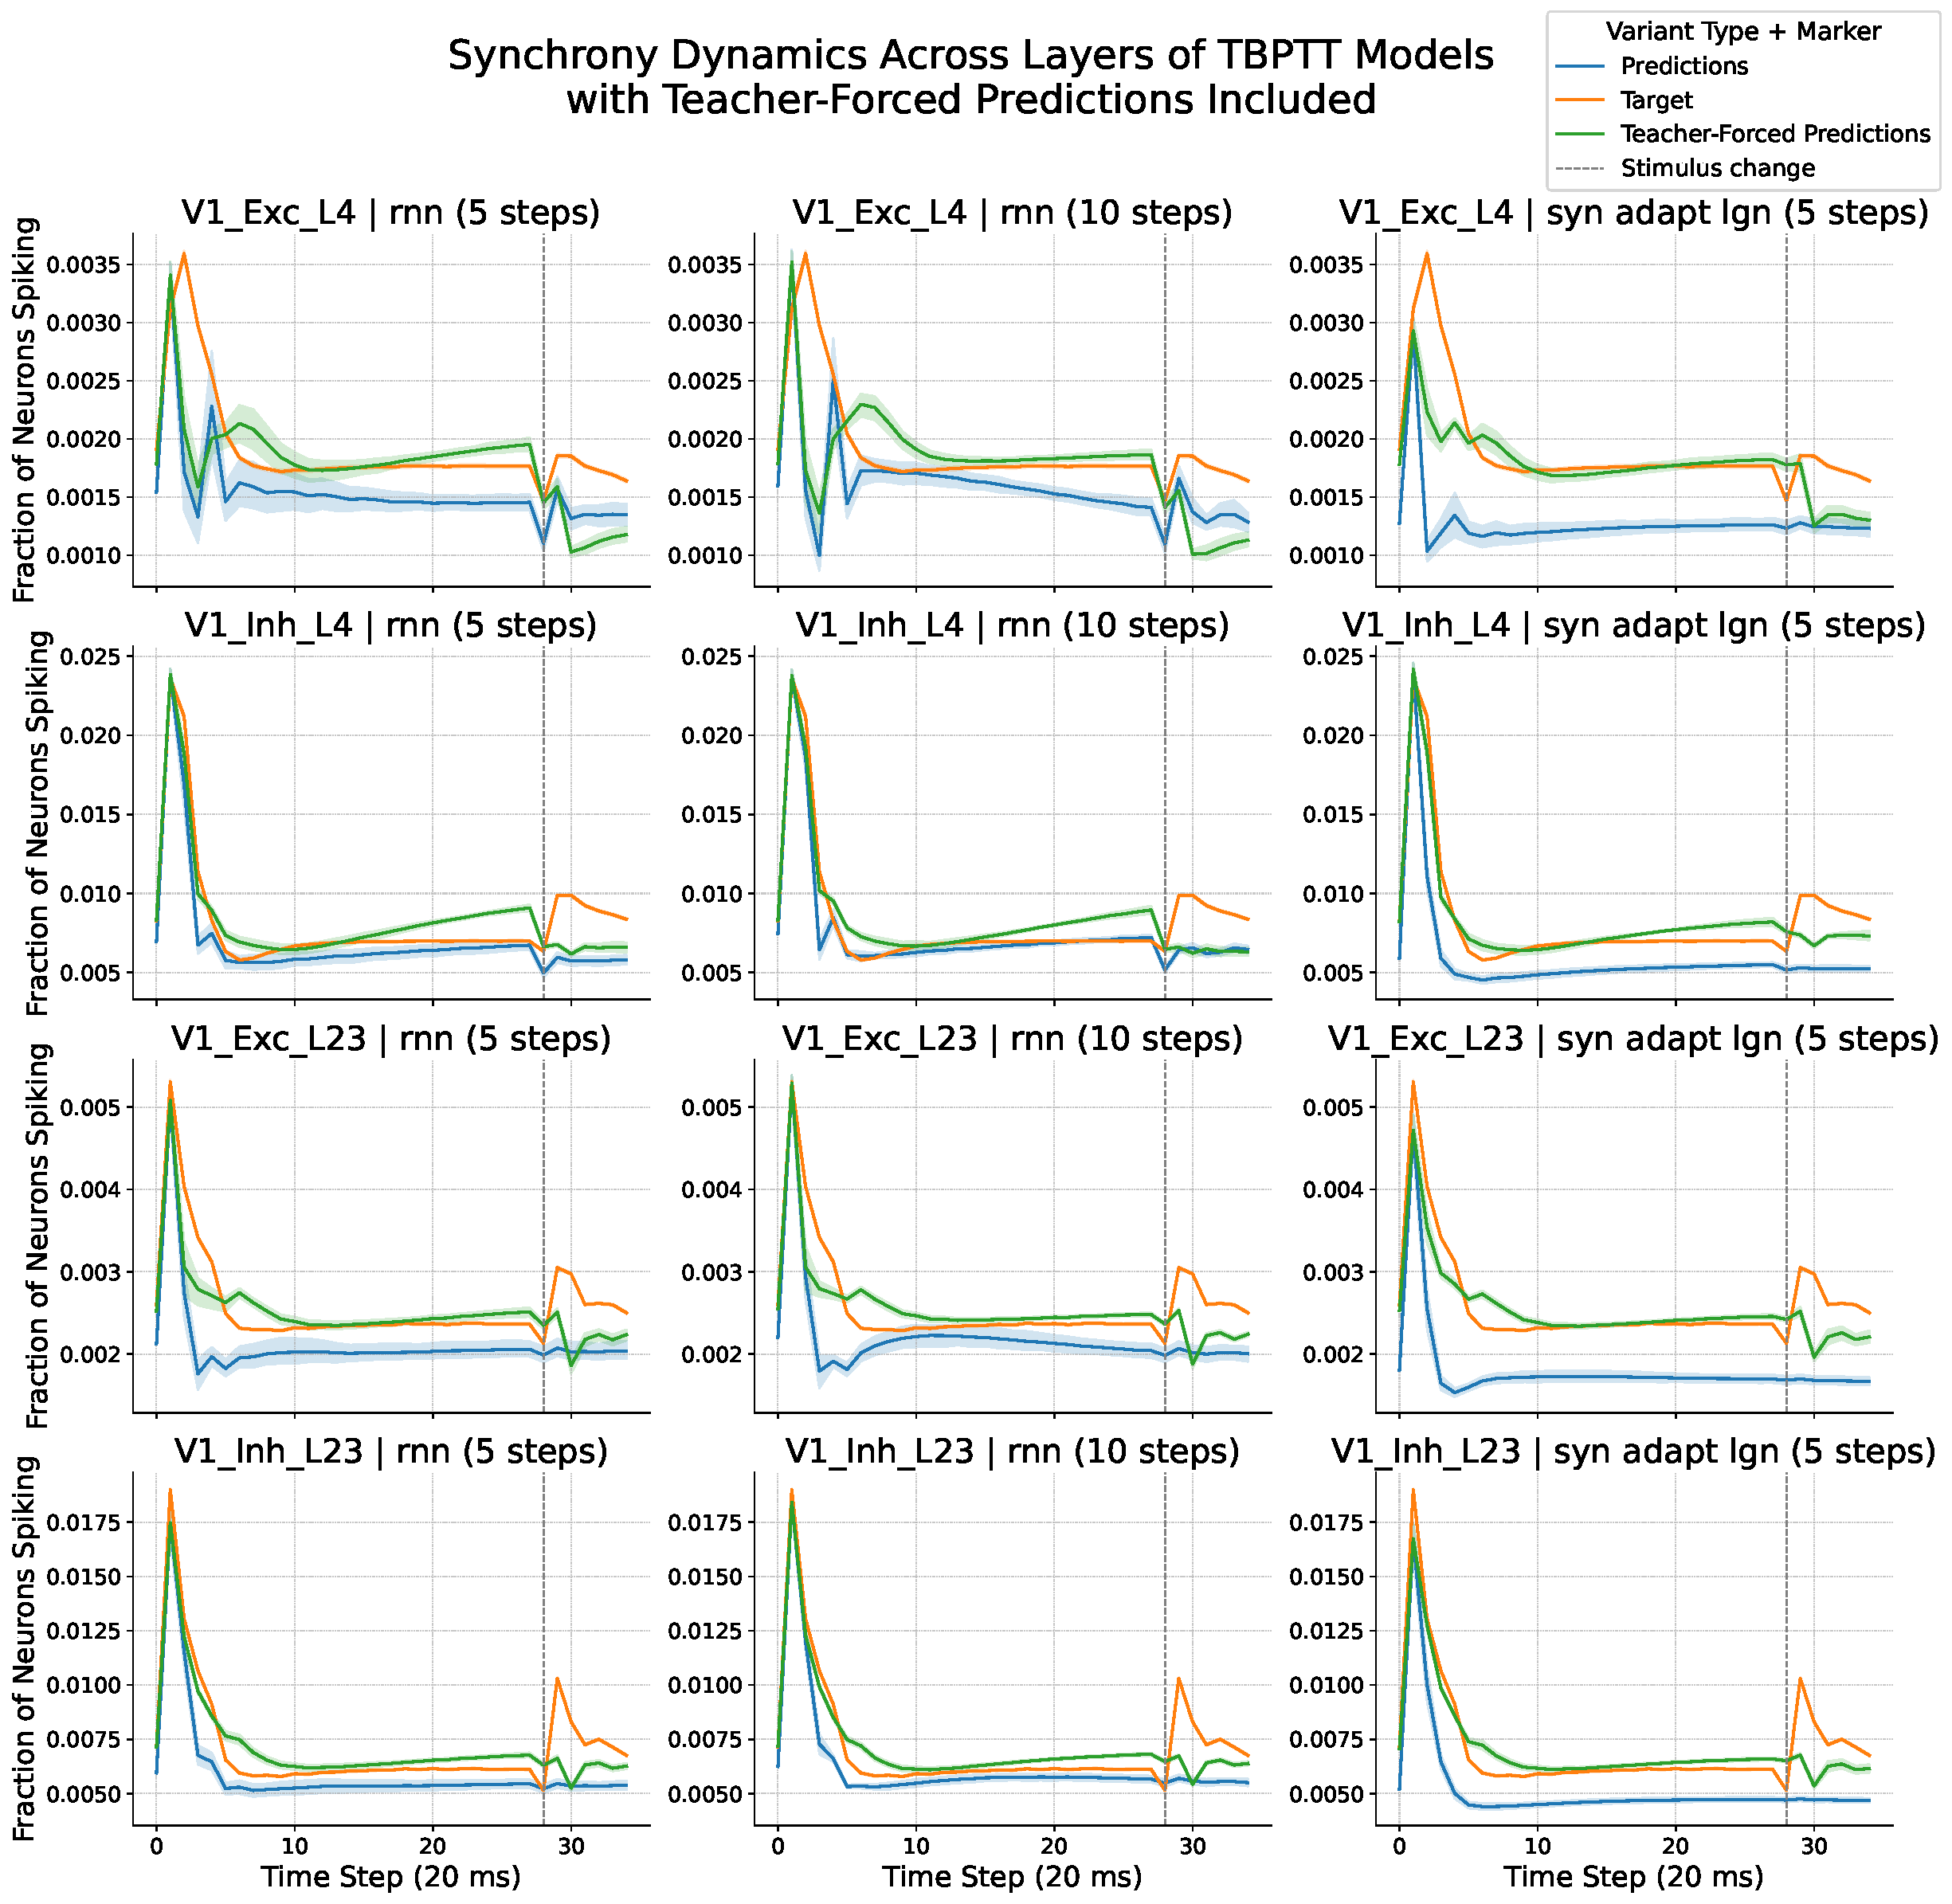
\includegraphics[width=\linewidth]{img/plots/tbptt_models_forced_included_model_synchrony_curve.pdf}
    \caption{Mean temporal spiking dynamics curves of all TBPTT-trained model variants under both free and teacher-forced prediction conditions, compared to the target temporal spiking dynamics curve. Curves are averaged across all trials and model subsets. Error bars represent standard deviation. The dashed vertical line indicates the transition from natural to blank stimuli.}
    \label{fig:free_vs_teacher_forced_synchrony}
\end{figure}

From the temporal spiking dynamics curves, we observe a modest improvement in temporal prediction accuracy during the early stages of natural stimulus presentation and at the transition to the blank stimulus phase. However, the models still struggle to replicate the elevated spontaneous activity observed in the blank phase of the target data. There is, however, a subtle increase in dynamic range during these stages, which may indicate potential for further improvement.

One notable discrepancy is observed in the teacher-forced predictions of RNN variants without synaptic depression, particularly in layer IV, where predictions deviate from the target during the later stages of natural stimulus presentation. 

An especially interesting case is the teacher-forced output of the synaptic depression model. This variant demonstrates the strongest overall alignment with the target temporal spiking dynamics curve across all TBPTT-trained models—a result also reflected in the population spike count correlation coefficients shown in Figure~\ref{fig:boxplot_models_pearson_synchrony_different_layers}. This performance may indicate that, despite the training challenges discussed previously, the model is capable of superior temporal modeling when appropriately guided.

\subsubsection{Drift Between Temporal Spiking Dynamics Curves of Teacher-Forced and Free Predictions}
\label{subsubsec:drift_teacher_free_synchrony}

In the final part of this section, we examine the difference between teacher-forced and free prediction temporal spiking dynamics curves, referred to here as \emph{drift}. This metric quantifies how model behavior diverges over time when guided by ground truth states versus when operating autonomously. The drift curves for each layer are shown in Figure~\ref{fig:teacher_forced_free_drift}.

\begin{figure}
    \centering
    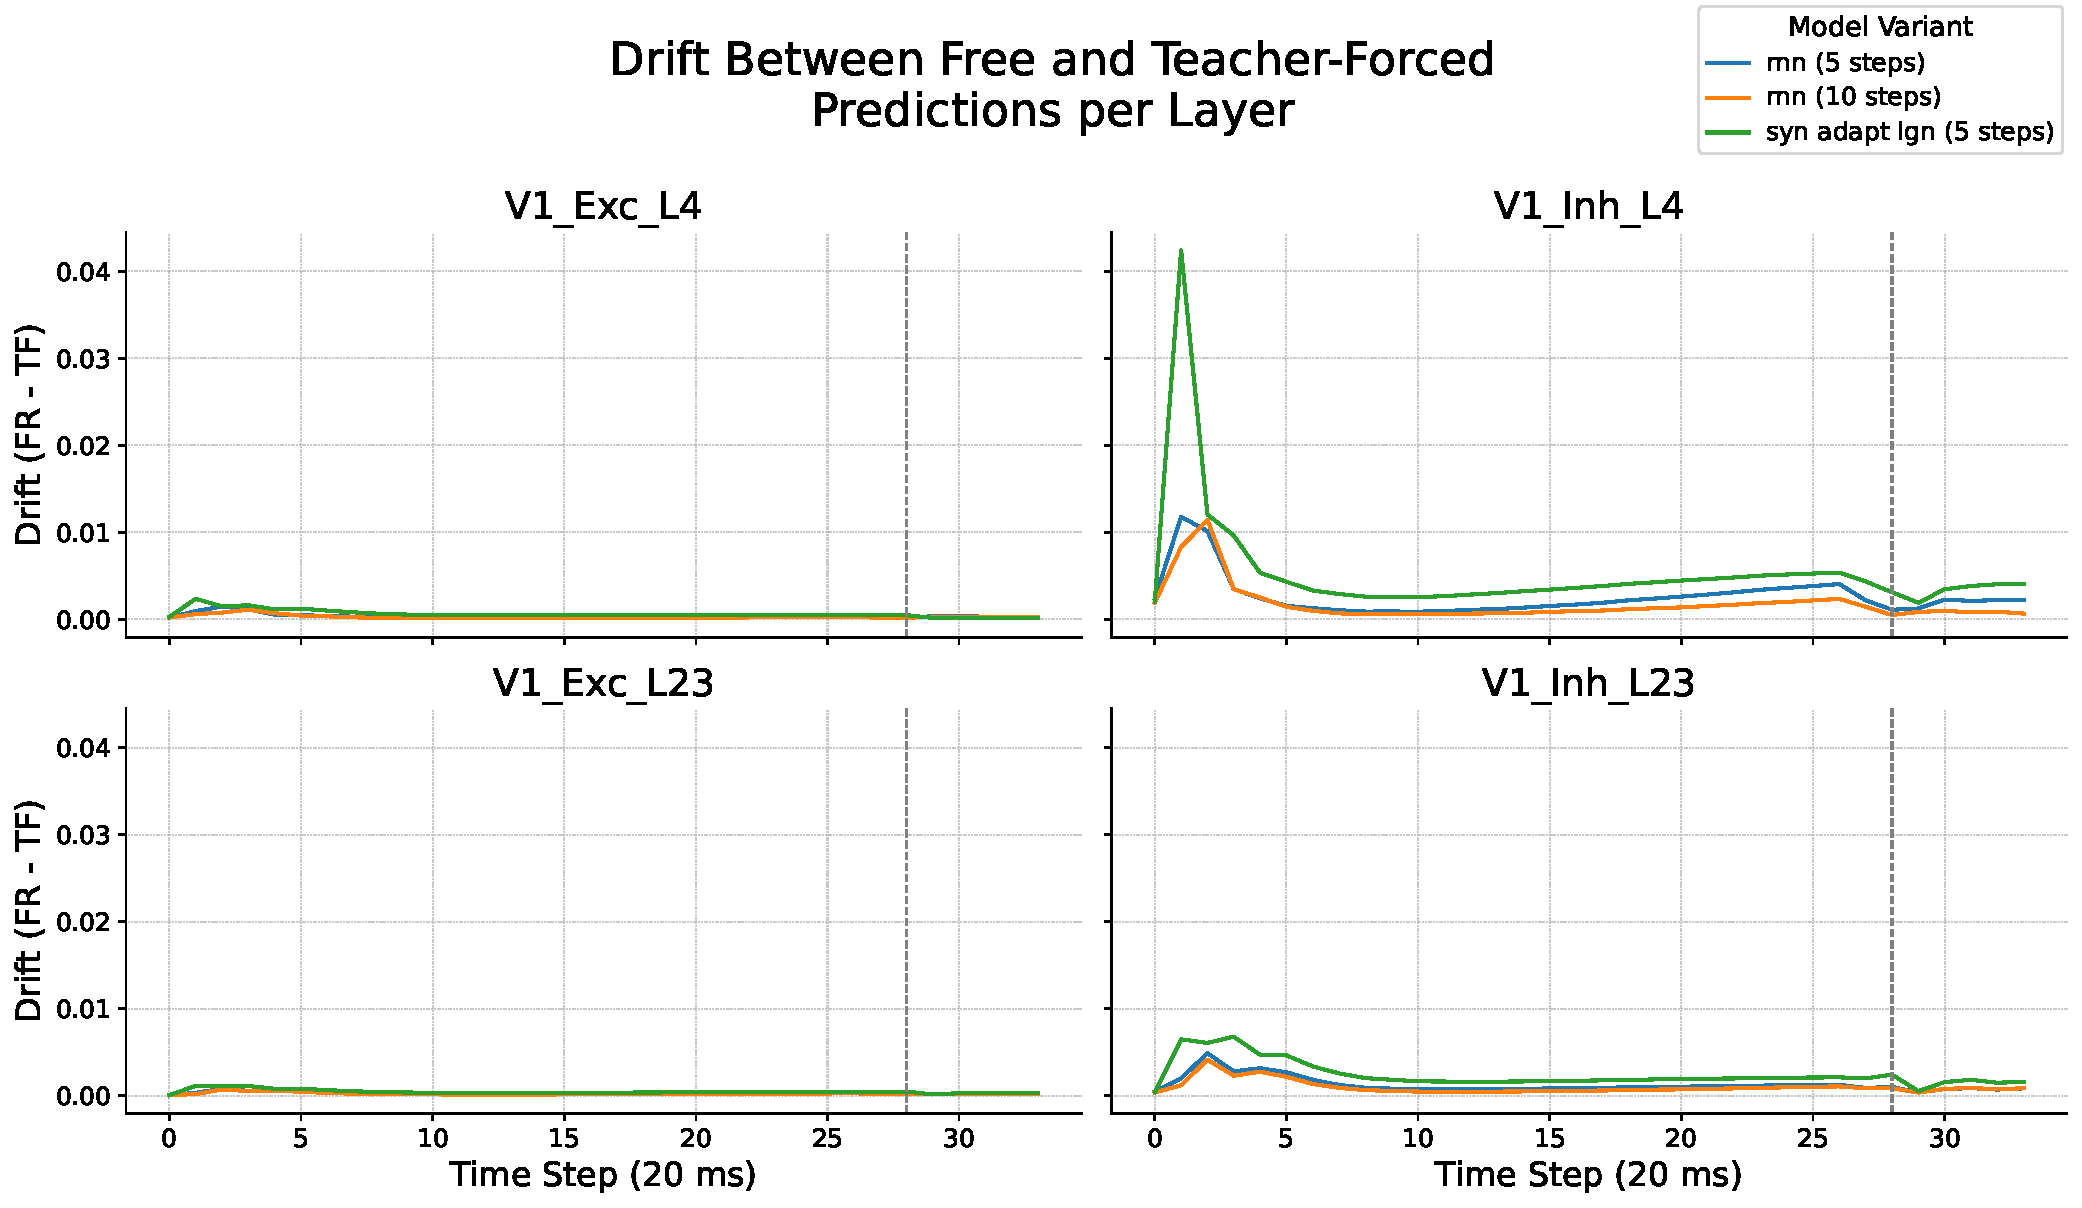
\includegraphics[width=\linewidth]{img/plots/temporal_drift_forced_free.pdf}
    \caption{Temporal evolution of the difference ("drift") between teacher-forced and free prediction temporal spiking dynamics curves across the experimental timeline, shown separately for each model layer. Results are averaged across all trials for TBPTT-trained models.}
    \label{fig:teacher_forced_free_drift}
\end{figure}

The greatest drift is observed during the initial natural stimulus phase, the period characterized by the highest neuronal activity. This pattern holds across all tested TBPTT models and highlights the challenge of modeling highly dynamic neuronal responses. Notably, the synaptic depression model exhibits the most pronounced drift throughout the experiment, reinforcing our earlier hypothesis regarding suboptimal training in this variant.

However, a promising finding is that the drift in all tested models stabilizes in the later stages of the stimulus sequence. This indicates that the models can adequately customize their responses and capture more stable temporal patterns once the initial burst of activity subsides. The discrepancy between teacher-forced and free predictions appears to be most critical in the highly dynamic early phases.

These observations suggest that the synaptic depression model holds strong potential for modeling biologically realistic temporal dynamics. Optimizing its training procedure, potentially through extended training, better hyperparameter tuning, or alternative optimization strategies, may substantially improve its performance.

\subsection{Hyperparameter Grid Search}
\label{subsec:hyperparameter_grid_search}

This section provides a brief overview of the hyperparameter grid search procedure conducted to support model evaluation. Due to computational constraints, all grid searches were performed on a single model subset variant different from the subsets selected for evaluation. Details regarding the selection of the validation dataset are outlined in Section~\ref{subsubsec:test_dataset}.

\subsubsection{Simple Model Grid Search}
\label{subsubsec:simple_model_grid_search}

Given the lightweight nature of the simple model in terms of both architecture and computational requirements, we were able to perform a comprehensive grid search over a range of learning rates. The training for each configuration was conducted for 10 epochs. Results for the simple (tanh) and simple (leakytanh) activation variants are presented in Tables~\ref{tab:grid_simple_tanh} and~\ref{tab:grid_simple_leakytanh}, respectively.

\begin{table}
    \centering\footnotesize\sf
    \begin{tabular}{ccc}
    \toprule
    lr & N-CC & P-CC \\
    \midrule
    0.000008 & 0.350904 & 0.285114 \\
    0.000005 & 0.350027 & 0.284416 \\
    0.000010 & 0.270970 & 0.220144 \\
    0.000025 & 0.187077 & 0.151972 \\
    0.000050 & 0.114566 & 0.093056 \\
    0.000500 & 0.097858 & 0.079533 \\
    0.000075 & 0.077174 & 0.062676 \\
    0.000100 & 0.037527 & 0.030460 \\
    \bottomrule
    \end{tabular}
    \caption{\textbf{Grid Search Summary for simple (tanh) Model.} Summary of normalized (N-CC) and Pearson (P-CC) correlation results for different learning rates (lr).}
    \label{tab:grid_simple_tanh}
\end{table}

\begin{table}
    \centering\footnotesize\sf
    \begin{tabular}{ccc}
    \toprule
    lr & N-CC & P-CC \\
    \midrule
    0.000100 & 0.878693 & 0.714005 \\
    0.000075 & 0.877059 & 0.712670 \\
    0.000050 & 0.872625 & 0.709055 \\
    0.000500 & 0.794590 & 0.645656 \\
    0.000025 & 0.294032 & 0.238913 \\
    0.000010 & 0.010441 & 0.008462 \\
    0.000005 & 0.001354 & 0.001069 \\
    0.000008 & 0.000050 & 0.000018 \\
    \bottomrule
    \end{tabular}
    \caption{\textbf{Grid Search Summary for simple (leakytanh) Model.} Summary of normalized (N-CC) and Pearson (P-CC) correlation results for different learning rates (lr).}
    \label{tab:grid_simple_leakytanh}
\end{table}

Although no particularly surprising patterns emerged during the grid search, one notable outcome was that the optimal learning rate for the simple (leakytanh)variant was significantly higher than that for the tanh variant. Interestingly, the performance trends with respect to learning rate were nearly opposite: the tanh model performed best with lower learning rates, while the leakytanh variant achieved better performance with higher ones.

Ultimately, we selected a learning rate of 0.0000075 for the tanh variant and 0.000075 for the leakytanh variant in our evaluation experiments. These choices were based on a combination of grid search results and empirical insights gained during model development, and differ only slightly from the highest-performing configurations.

\subsubsection{DNN Joint Model Grid Search}
\label{subsubsec:dnn_joint_grid_search}
We extended our hyperparameter grid search to the dnn joint model, using a broader set of parameters as outlined in Table~\ref{tab:grid_dnn_joint}. Each configuration was trained for 10 epochs using the same model subset variant as in grid search for the simple model.

\begin{table}
    \centering\footnotesize\sf
    \begin{tabular}{cccccc}
    \toprule
    lr & n-ls & n-nl & n-res & N-CC & P-CC \\
    \midrule
    0.000010 & 10 & 3 & True & 0.880114 & 0.715163 \\
    0.000010 & 10 & 7 & True & 0.879289 & 0.714492 \\
    0.000008 & 10 & 3 & True & 0.878549 & 0.713885 \\
    0.000008 & 10 & 7 & True & 0.878224 & 0.713618 \\
    0.000008 & 10 & 5 & True & 0.877150 & 0.712746 \\
    0.000010 & 5 & 5 & True & 0.876449 & 0.712174 \\
    0.000010 & 5 & 7 & True & 0.871925 & 0.708491 \\
    0.000010 & 10 & 5 & True & 0.871830 & 0.708410 \\
    0.000008 & 5 & 5 & True & 0.866316 & 0.703933 \\
    0.000010 & 5 & 3 & True & 0.860474 & 0.699177 \\
    0.000008 & 5 & 7 & True & 0.857937 & 0.697110 \\
    0.000010 & 5 & 5 & False & 0.854195 & 0.694092 \\
    0.000010 & 10 & 3 & False & 0.825813 & 0.670711 \\
    0.000008 & 10 & 3 & False & 0.813353 & 0.660599 \\
    0.000010 & 10 & 5 & False & 0.798817 & 0.648800 \\
    0.000010 & 5 & 3 & False & 0.766755 & 0.623028 \\
    0.000008 & 5 & 7 & False & 0.759580 & 0.617220 \\
    0.000008 & 10 & 7 & False & 0.751363 & 0.610289 \\
    0.000008 & 5 & 5 & False & 0.723905 & 0.587979 \\
    0.000010 & 10 & 7 & False & 0.722965 & 0.587225 \\
    0.000008 & 10 & 5 & False & 0.626814 & 0.509143 \\
    0.000008 & 5 & 3 & True & 0.295512 & 0.240123 \\
    0.000008 & 5 & 3 & False & 0.008394 & 0.006809 \\
    0.000010 & 5 & 7 & False & -0.259292 & -0.210666 \\
    \bottomrule
    \end{tabular}
    \caption{\textbf{Grid Search Summary for dnn joint Model.} Summary of normalized (N-CC) and Pearson (P-CC) correlation results for different learning rates (lr), neuron module layer size (n-ls), number of layers of neuron module (n-nl) and presence of residual connection in neuron module (n-res).}
    \label{tab:grid_dnn_joint}
\end{table}

The grid search results clearly demonstrate the benefit of residual connections within the neuron modules. Residual-enabled models consistently outperformed their non-residual counterparts in both normalized and Pearson correlation metrics. Empirically, we also observed enhanced training stability, reduced overfitting, and more consistent convergence behavior. Based on these findings, we applied residual connections to all modules in subsequent model configurations.

Regarding the number of layers, the results indicate minimal variation in performance across configurations, though five layers showed the most stable performance overall. This matches observations made during earlier development stages, leading us to select five layers for final evaluation.


For layer size, a size of 10 consistently performed better across configurations. While larger layer sizes could potentially offer additional capacity, our empirical testing did not show improvements. Moreover, larger models significantly increase memory requirements, particularly under TBPTT training. Although this is less of a concern for feed-forward DNNs, we opted to retain the layer size of 10 for both performance and efficiency.

We selected a learning rate of 0.00001 for final evaluation based on its consistently strong performance during the grid search. This choice aligns well with our prior empirical observations regarding training dynamics.

Finally, it is important to note that we did not conduct a grid search for the dnn separate model due to computational resource constraints. This omission may partially explain the inconsistent behavior observed in that model during evaluation.

\subsubsection{RNN Separate Model Grid Search}
\label{subsubsec:rnn_grid_search}
We conducted a grid search for the rnn separate model, focusing primarily on the number of TBPTT (Truncated Backpropagation Through Time) time steps. The layer size was fixed at 10 and the number of layers at 3, based on their reliable performance in the dnn joint model grid search. The choice of a lightweight configuration, particularly with only 3 layers, was driven by the high computational and memory demands associated with recurrent modules, especially when using longer TBPTT sequences.

Due to these resource constraints, we limited the search space and acknowledge that the chosen configurations may not represent a global optimum. Each model variant was trained for 40 epochs to better accommodate the slower convergence of RNNs. Results of this grid search are summarized in Table~\ref{tab:grid_rnn_separate}. Note that we excluded the rnn joint variant from this study, as our goal is to prioritize biologically plausible architectures, and the joint variant conflicts with this aim.

\begin{table}
    \centering\footnotesize\sf
    \begin{tabular}{cccc}
    \toprule
    lr & n-tbptt & N-CC & P-CC \\
    \midrule
    0.000030 & 10 & 0.933978 & 0.758967 \\
    0.000030 & 5 & 0.932902 & 0.758091 \\
    0.000050 & 10 & 0.932787 & 0.757994 \\
    0.000010 & 5 & 0.914351 & 0.743027 \\
    0.000030 & 20 & 0.913769 & 0.742504 \\
    0.000010 & 10 & 0.911943 & 0.741078 \\
    0.000050 & 40 & 0.911054 & 0.740291 \\
    0.000050 & 5 & 0.885195 & 0.719318 \\
    0.000010 & 20 & 0.873075 & 0.709455 \\
    0.000050 & 20 & 0.829914 & 0.674317 \\
    0.000030 & 40 & 0.689550 & 0.560315 \\
    0.000010 & 40 & 0.281750 & 0.228879 \\
    \bottomrule
    \end{tabular}
    \caption{\textbf{Grid Search Summary for rnn separate Model.} Summary of normalized (N-CC) and Pearson (P-CC) correlation results for different learning rates (lr) and number of TBPTT time steps (n-tbptt).}
    \label{tab:grid_rnn_separate}
\end{table}

The grid search yielded an unexpected finding: models with higher TBPTT step counts generally performed worse than those with 5 or 10 steps. We hypothesize that this is due to insufficient training time, longer TBPTT sequences likely require additional epochs to converge. This theory is supported by the performance of the model trained with 40 TBPTT steps and the highest learning rate (0.00005), which still achieved relatively competitive correlation scores.

Nevertheless, given the significant increase in computational cost associated with longer TBPTT sequences, we selected 5 and 10 steps as our evaluation standards. These configurations offered the best balance of performance and feasibility. As for the learning rate, 0.00003 was chosen for final evaluation, based on its consistent top performance in the tested scenarios.

\subsubsection{Synaptic Depression Grid Search}
\label{subsubsec:synaptic_depression_grid_search}
In the final section dedicated to grid search, we focus on the hyperparameters for the synaptic depression module. This part of the analysis was significantly limited by computational resources. Performing a comprehensive grid search on models with full synaptic depression, applied across all connected pairs of neuronal populations, is computationally intensive, particularly when applied with longer TBPTT sequences.

Although our original goal was to train each configuration for 40 epochs, we were only able to train for 20 epochs due to time and memory constraints. Similarly, the number of TBPTT steps had to be limited to 5 and 10. For the RNN neuron module, we used 3 layers of size 10 (as in the RNN grid search). To further manage resource demands, the synaptic depression modules was configured with just 2 layers of size 10. Grid search results are presented in Table~\ref{tab:grid_synaptic_adaptation}.

\begin{table}
    \centering\footnotesize\sf
    \begin{tabular}{cccc}
    \toprule
    lr & n-tbptt & N-CC & P-CC \\
    \midrule
    0.000030 & 5 & 0.904516 & 0.734752 \\
    0.000050 & 10 & 0.858861 & 0.697665 \\
    0.000010 & 5 & 0.826371 & 0.671237 \\
    0.000010 & 10 & 0.728944 & 0.592099 \\
    0.000050 & 5 & 0.678222 & 0.550937 \\
    0.000030 & 10 & -0.016808 & -0.013631 \\
    \bottomrule
    \end{tabular}
    \caption{\textbf{Grid Search Summary for synaptic depression Model.} Summary of normalized (N-CC) and Pearson (P-CC) correlation results for different learning rates (lr) and number of TBPTT time steps (n-tbptt).}
    \label{tab:grid_synaptic_adaptation}
\end{table}

The results reveal that the full synaptic depression model achieved a normalized CC of 0.90 using only 5 TBPTT steps and 20 training epochs. This is an encouraging outcome, suggesting that with longer training durations and more extensive hyperparameter tuning, the model could offer significant performance improvements.

This incomplete grid search also partially explains the poor performance of the syn adapt lgn (5 steps) model. In that case, synaptic depression was applied only to LGN connections, a simplification necessitated by resource constraints. During evaluation, the LGN-only variant demonstrated slower learning and required more epochs to reach competitive correlation values.

Moreover, the limited training duration and use of only 5 TBPTT steps likely contributed to underfitting. This is further supported by the observation that teacher-forced predictions were significantly better for the synaptic depression model, a trend not observed in RNN variants without synaptic depression. These findings collectively suggest that synaptic depression holds substantial promise, and that future work with better computational resources could unlock its full potential.

\subsection{Impact of Training Dataset Size on Model Performance}
\label{subsec:train_size_dataset_depencdency}
In the final part of our experimental analysis, we briefly examine how the size of the training dataset influences model performance, as measured by normalized cross-correlation (CC). For this investigation, we utilized the dnn joint model due to its relatively low computational cost and its inclusion of a neuron module in the architecture. Each model was trained for 10 epochs using the same setup as described in Table~\ref{tab:evaluation_setup}, and trained on the same model subset as used in the grid search.

Our initial goal was to evaluate the model's performance across the full range of training dataset sizes, increasing in 2\% increments. However, due to computational limitations, we were only able to evaluate model performance for training dataset ratios in the range $[0.02, 0.54]$ with step increments of 0.02. The results are visualized in Figure~\ref{fig:train_size_cc_norm_dependency}.

\begin{figure}
    \centering
    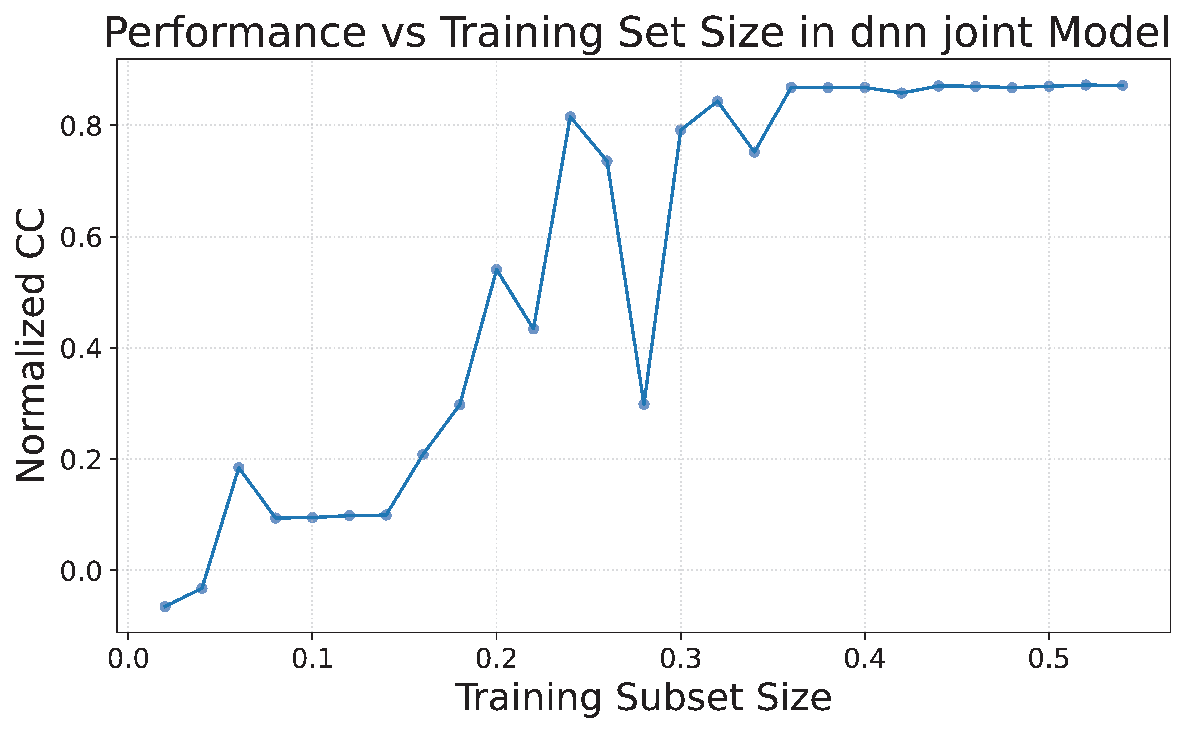
\includegraphics[width=0.8\linewidth]{img/plots/train_size_performance_dependency.pdf}
    \caption{Dependency of normalized CC on training dataset size for the dnn joint model using the hyperparameter configuration from Table~\ref{tab:evaluation_setup}. Due to computational constraints, only dataset sizes up to 54\% of the original training data were tested.}
    \label{fig:train_size_cc_norm_dependency}
\end{figure}

The results indicate that normalized CC values stabilize around 36\% of the training dataset. Beyond this point, additional data does not appear to yield significant improvements in performance. This finding suggests that increasing the size of the training dataset beyond this threshold is unlikely to provide meaningful benefits for the dnn joint model, at least within the constraints of a feed-forward architecture.

That said, this analysis was limited to a single model type. Further investigation is needed to determine whether this trend holds across more complex architectures, particularly those incorporating recurrent or adaptive components. Additionally, our dataset is derived from a limited range of experimental conditions. Exploring alternative stimulus types, such as natural movies or other paradigms discussed in Section~\ref{subsec:stimulus}, may offer further opportunities to enhance model generalization and performance.
